%\section{Simulaatiot}
\section{Antenna simulations}
\label{sec:simulations}

\begin{itemize}
\item[--]simulointimallin kehittyminen
\item[--]referenssitesti (ei metallilevyä)
\item[--]simulointien tulokset
\item[--]
\end{itemize}






\subsection{Simulations with plain model}
\label{sec:sim_plain}
Designing antenna structures was started with a plain and simple simulation model. Besides the antennas under test, the model consisted of only the metallic back cover, and FR4-substrate with a metallic sheet as a display. The reason for keeping the model simple was to reduce simulation times, and to learn how different structures perform in the presence of the metal cover. To clarify, from now on, main antenna refers to the first cellular antenna to be designed, and diversity antenna to the second one, regardless how their performances compare to each other. 

Tested antenna structures were mainly placed in the sides of the phone, due to integrability to the side metals in the final design. Besides suitable antenna locations, also antenna shapes, dimensions, and feed positions were investigated. Also structures of antenna elements were kept as simple as possible in order to follow the effects of each parameter in an efficient way. The simple model was used until a promising structure for the main antenna was found. 

\subsubsection{Effect of metal cover}
\label{sec:metal_effect}
The main point of interest, as well as the main challenge, is the metal cover and how it affects the antenna performance. To demonstrate the complexity of this design project, simulations to test the effect of the metal were run. Since this test was just an example, simulation model was kept simple. A long, L-shaped antenna completely covering one long side and one short side, with a little square on the corner was used in this test. Models are shown in Figure \ref{fig:metal_vs_nometal_model}.

\begin{figure}[H]
    \centering
    \begin{subfigure}[b]{0.49\textwidth}
    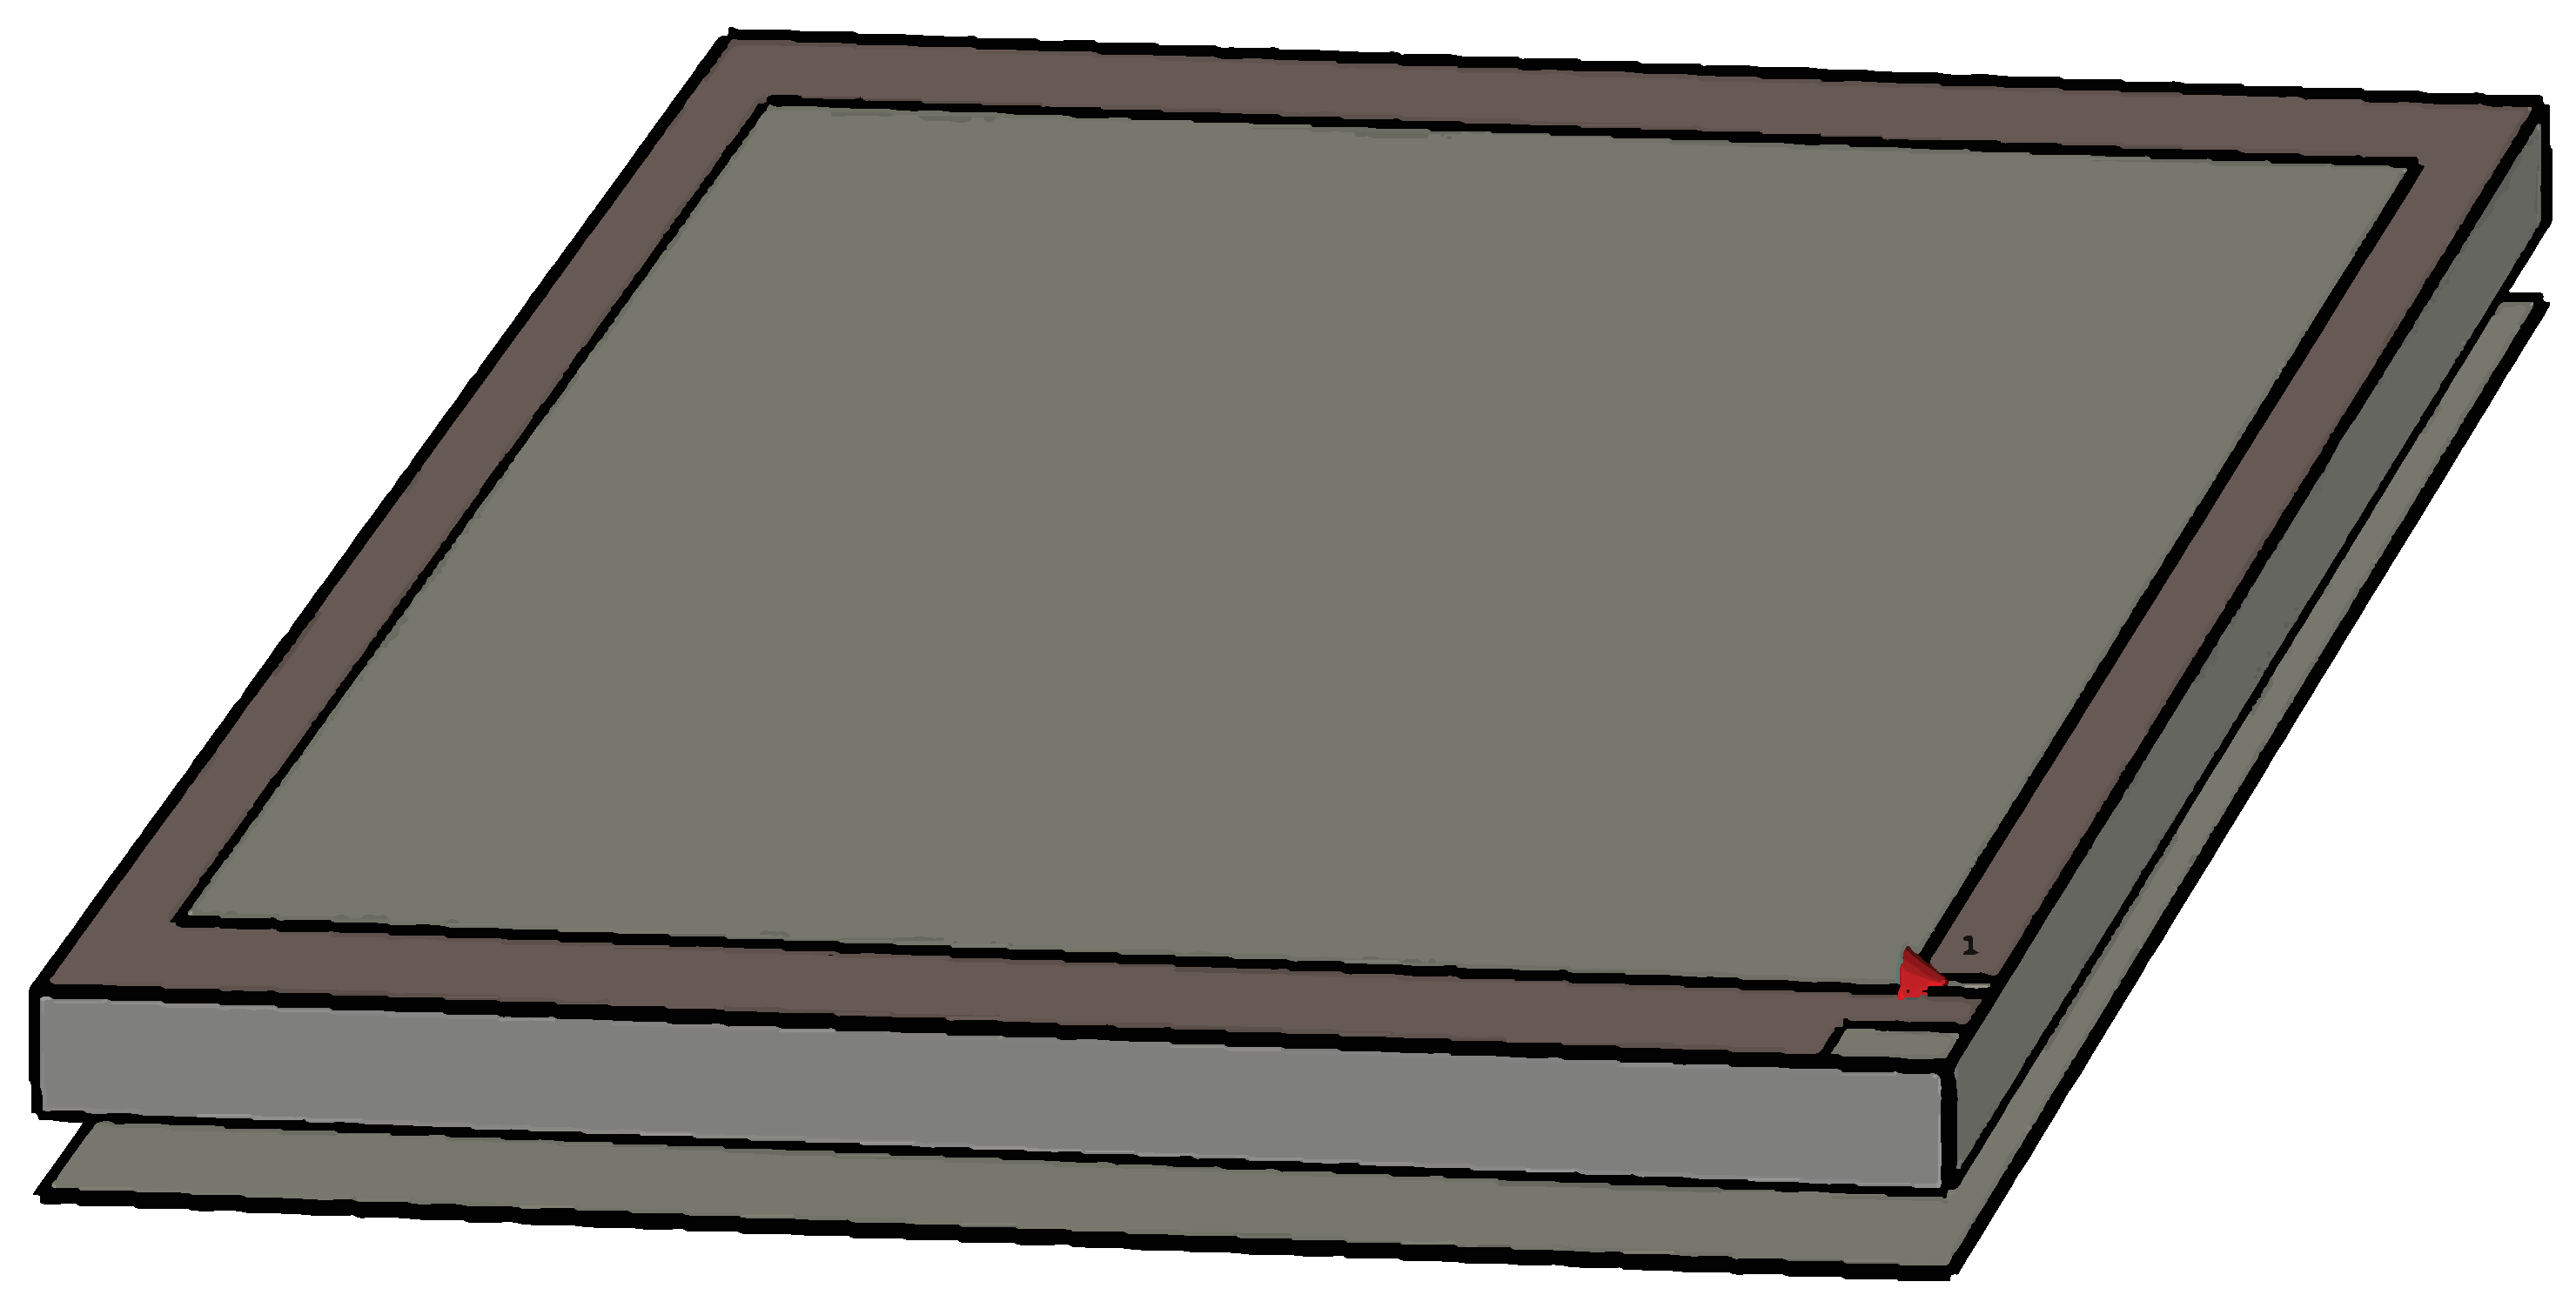
\includegraphics[width=\textwidth]{img/metal_cover.eps}
    \caption{With metal cover.}
    \label{fig:metal_cover}
    \end{subfigure}
    \begin{subfigure}[b]{0.49\textwidth}
    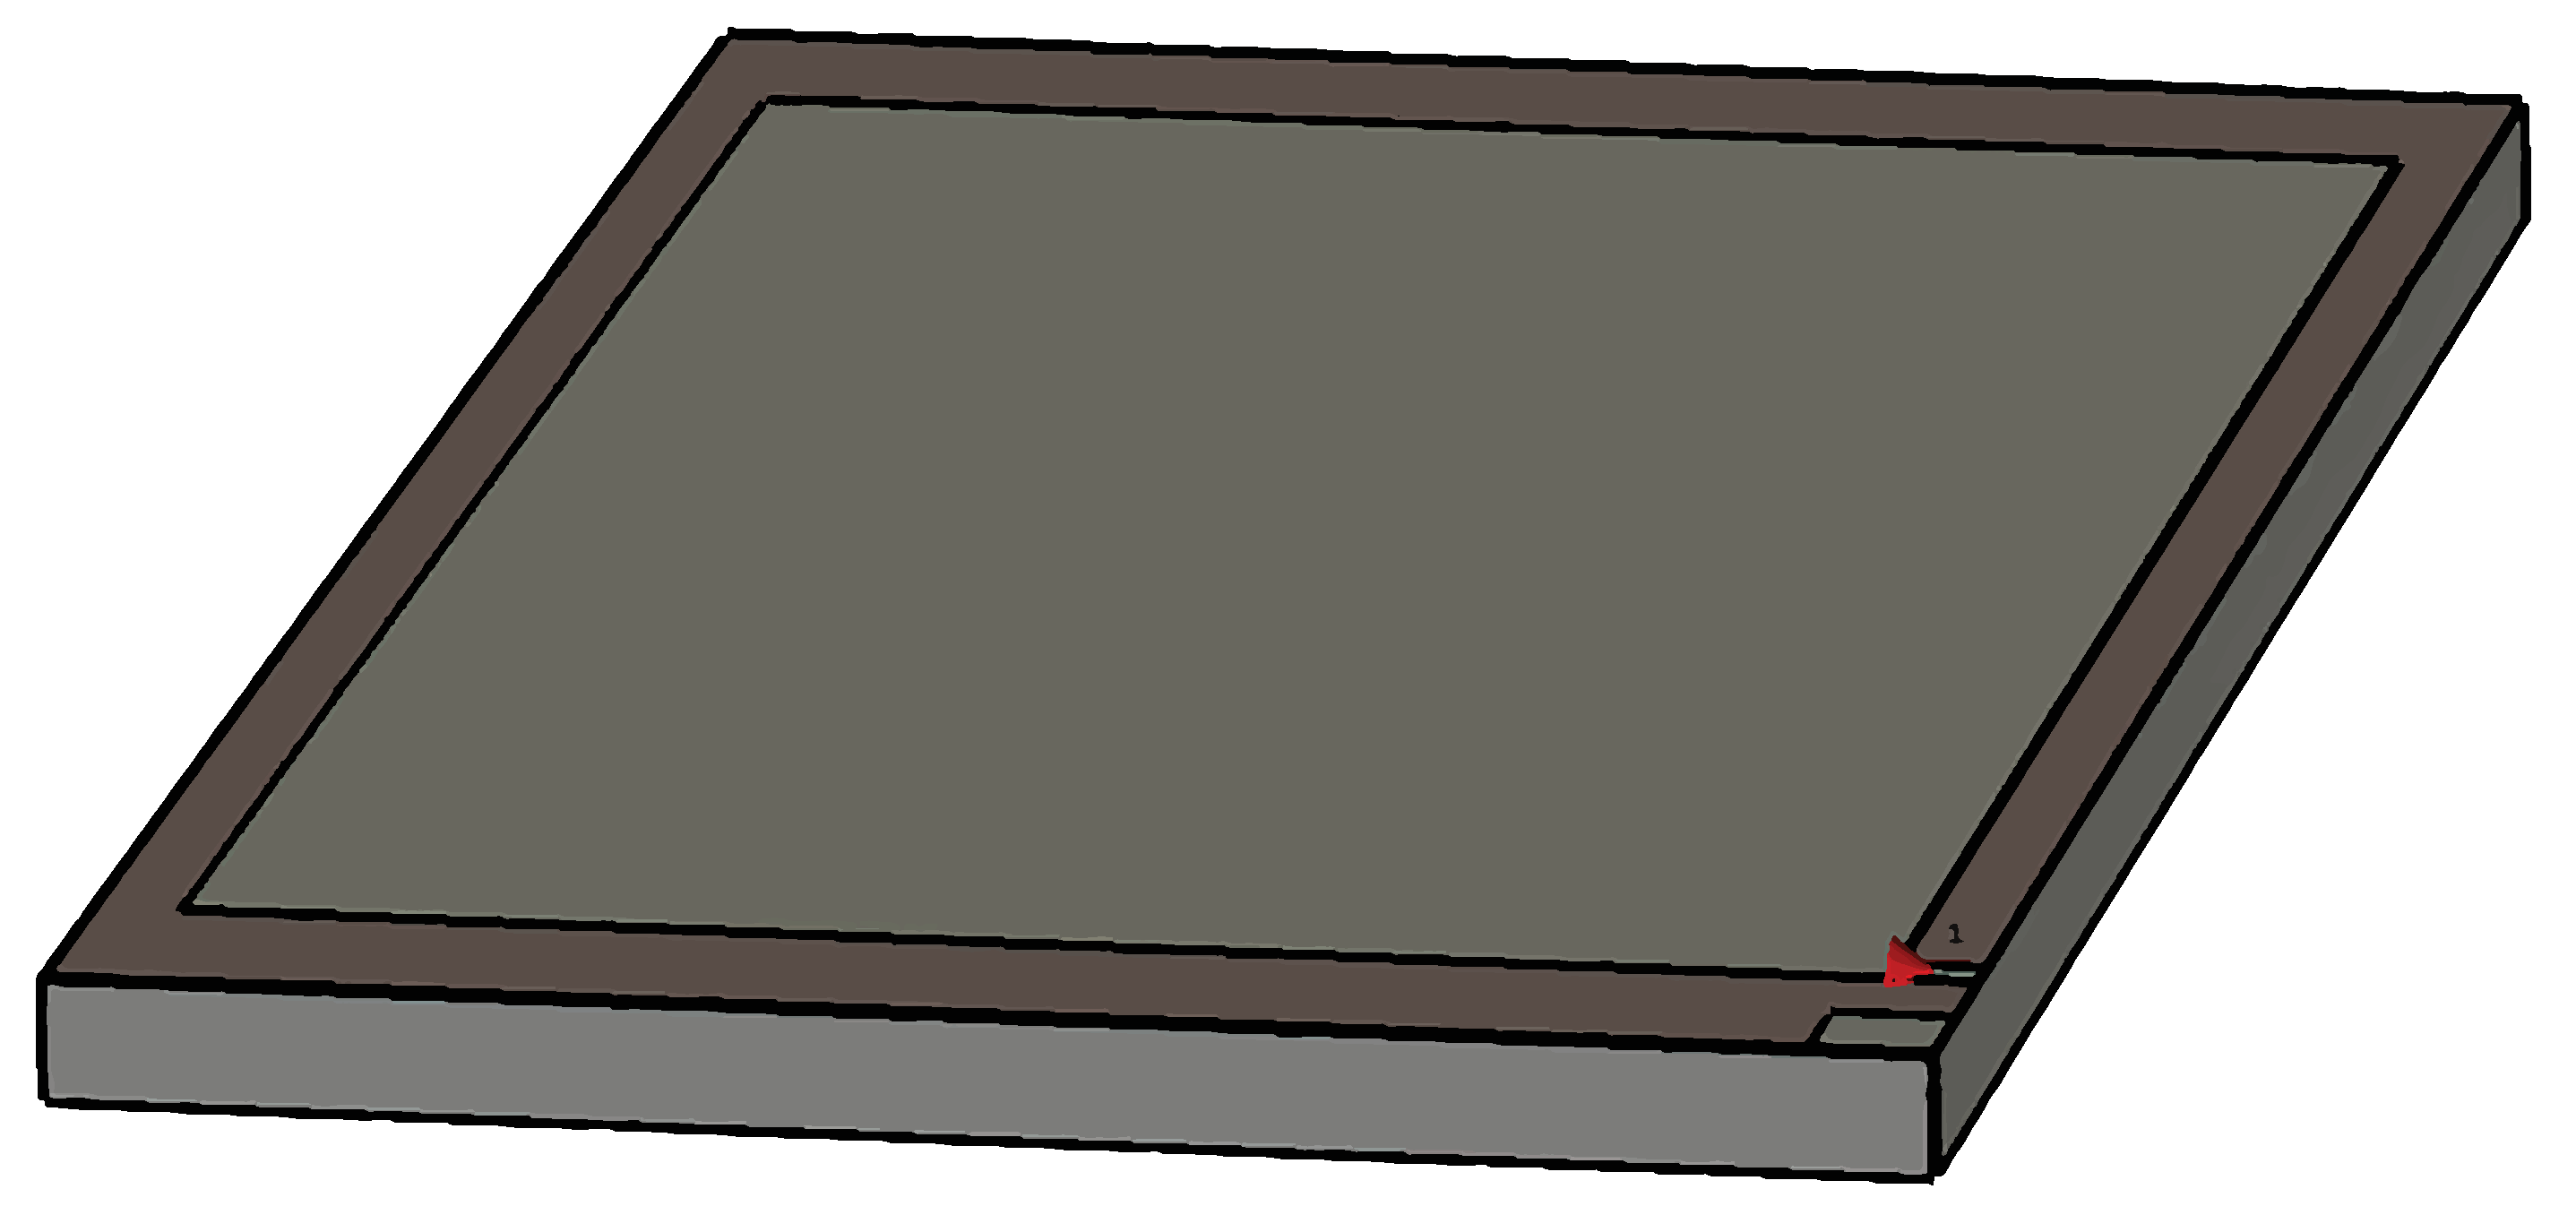
\includegraphics[width=\textwidth]{img/no_metal_cover.eps}
    \caption{Without metal cover.}
    \label{fig:nometal_cover}
    \end{subfigure}
    \caption{Simulation models used to test the effect of metal cover. Antenna element is on the side of the phone.}
    \label{fig:metal_vs_nometal_model}
\end{figure}

Figure \ref{fig:metal_vs_nometal} shows the results from the CST-simulation. The effect of the metal cover can be seen clearly. The blue curve has a metallic back cover while the red, dashed one does not. Looking at the low band reveals a major difference. The aim of the matching level is $-5\,\db$ and that is almost achieved when the metal cover is taken away without any external matching networks. With metal cover the antenna resonates more with narrower peaks and has no desired matching level at any frequency. 

Figure \ref{fig:metal_vs_nometal_matched} presents the same simulations with 4-element matching circuit created with Optenni Lab. This time the difference is even larger. Without metal cover the desired matching level is exceeded by far. In contrary, adding matching circuit to the other case is not much of help. Even though the level is now more constant in the band, it is far from acceptable.

\begin{figure}[H]
    \centering 
    \begin{subfigure}[b]{0.49\textwidth}
        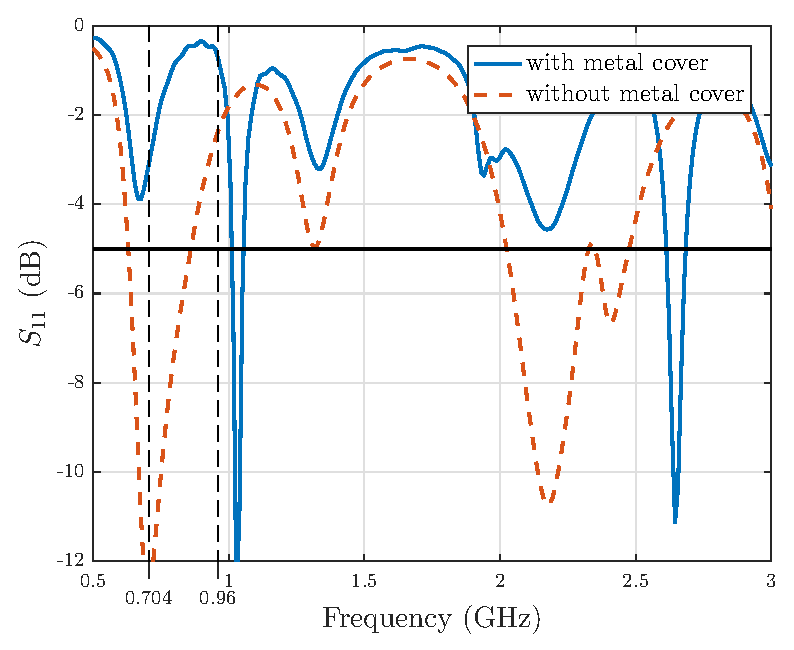
\includegraphics[width=\textwidth]{img/metal_vs_nometal.eps}
        \caption{Without matching circuit.}
        \label{fig:metal_vs_nometal}
    \end{subfigure}
    \begin{subfigure}[b]{0.49\textwidth}
        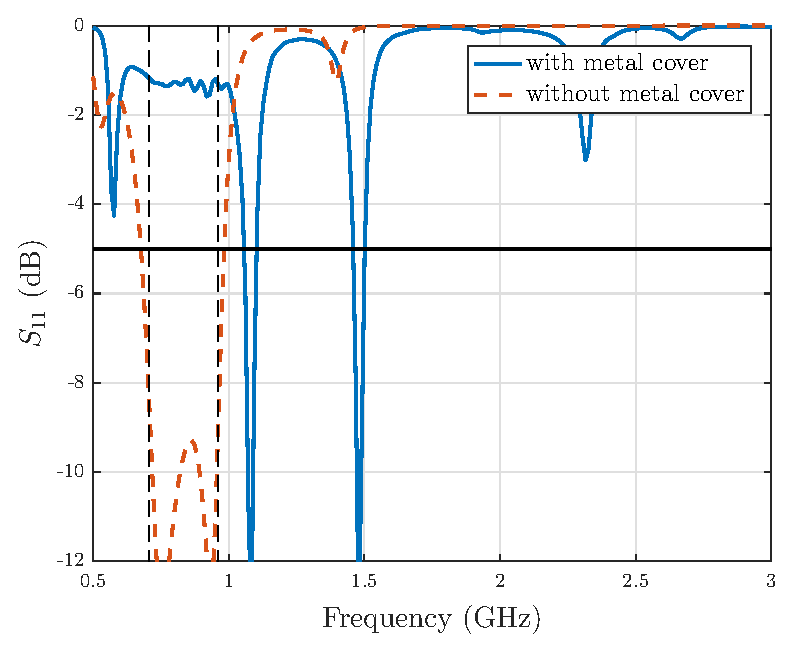
\includegraphics[width=\textwidth]{img/metal_vs_nometal_matched.eps}
        \caption{Matched antennas.}
        \label{fig:metal_vs_nometal_matched}
    \end{subfigure}
    \caption{Effect of the metal back cover on antenna performance.}
    \label{fig:metal_vs_nometal_results}
\end{figure}

\subsubsection{Study on the effects of different dimensions}
\label{sec:dimension_study}
As mentioned earlier in section \ref{sec:process}, antennas were designed and developed in the EM simulator. Each simulated design provided information that was useful for the following iterations. Gathering knowledge on how modifying different parts of an antenna affects the performance was critical since antennas in metal-covered mobile phones are not that much studied, as was presented in section \ref{sec:full_cover}.

The first interesting metric to investigate was the size of the antenna. This meant length ($l$) and width ($w$) of the antenna since all elements were considered as thin metallic sheets. The tested antennas were $2\,\milli\meter$ wide metal strips either on the long or the short side of the phone (see Figures \ref{fig:ant_length_long} and \ref{fig:ant_length_short}, respectively). In both cases everything else was kept constant except the length of antenna. 

\begin{figure}[H]
    \centering
    \begin{subfigure}[b]{0.49\textwidth}
        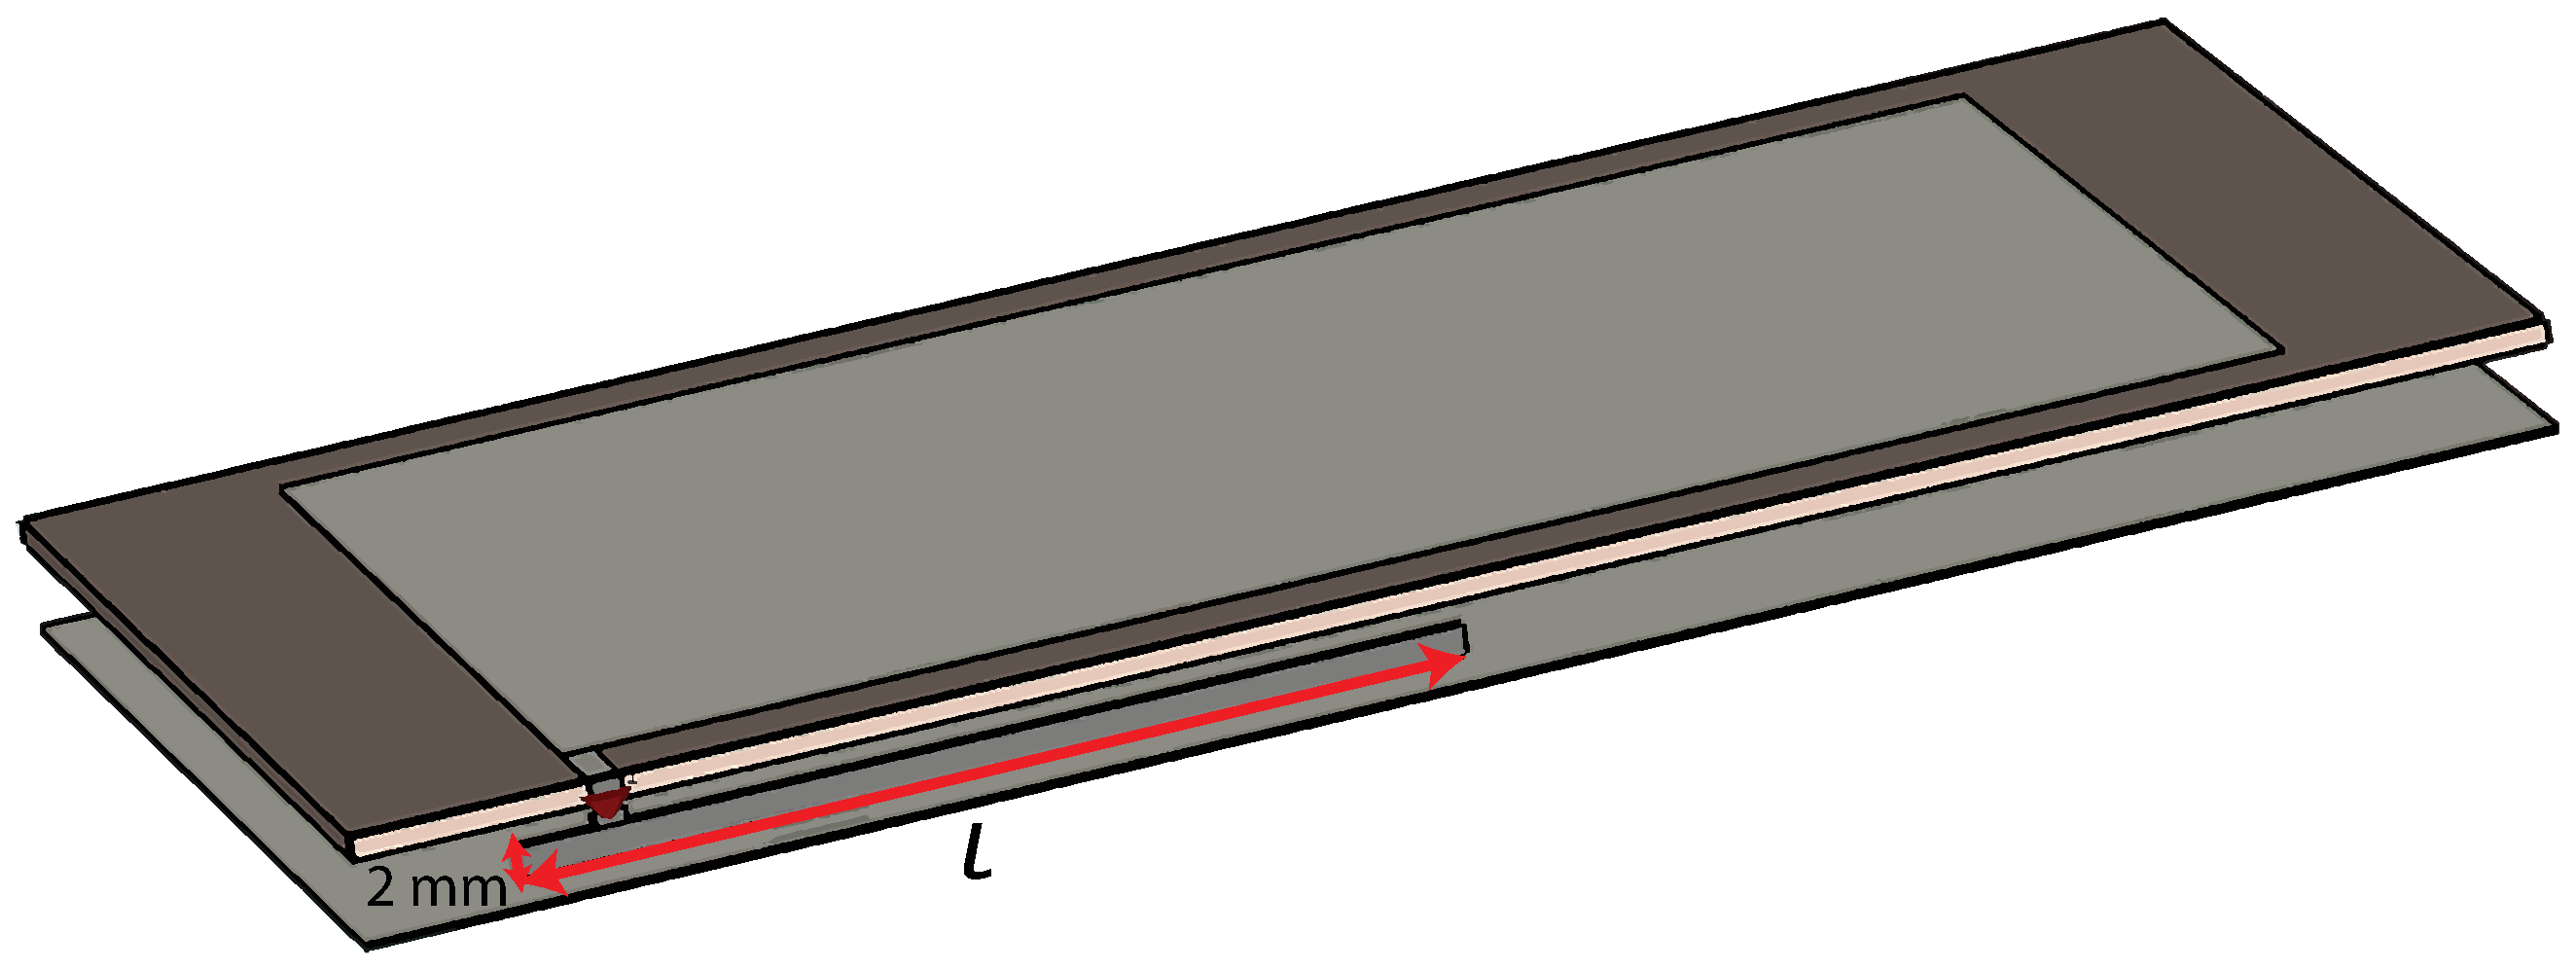
\includegraphics[width=\textwidth]{img/ant_length_long.eps}
        \caption{Antenna located on the side of the phone.}
        \label{fig:ant_length_long}
    \end{subfigure}
    \begin{subfigure}[b]{0.49\textwidth}
        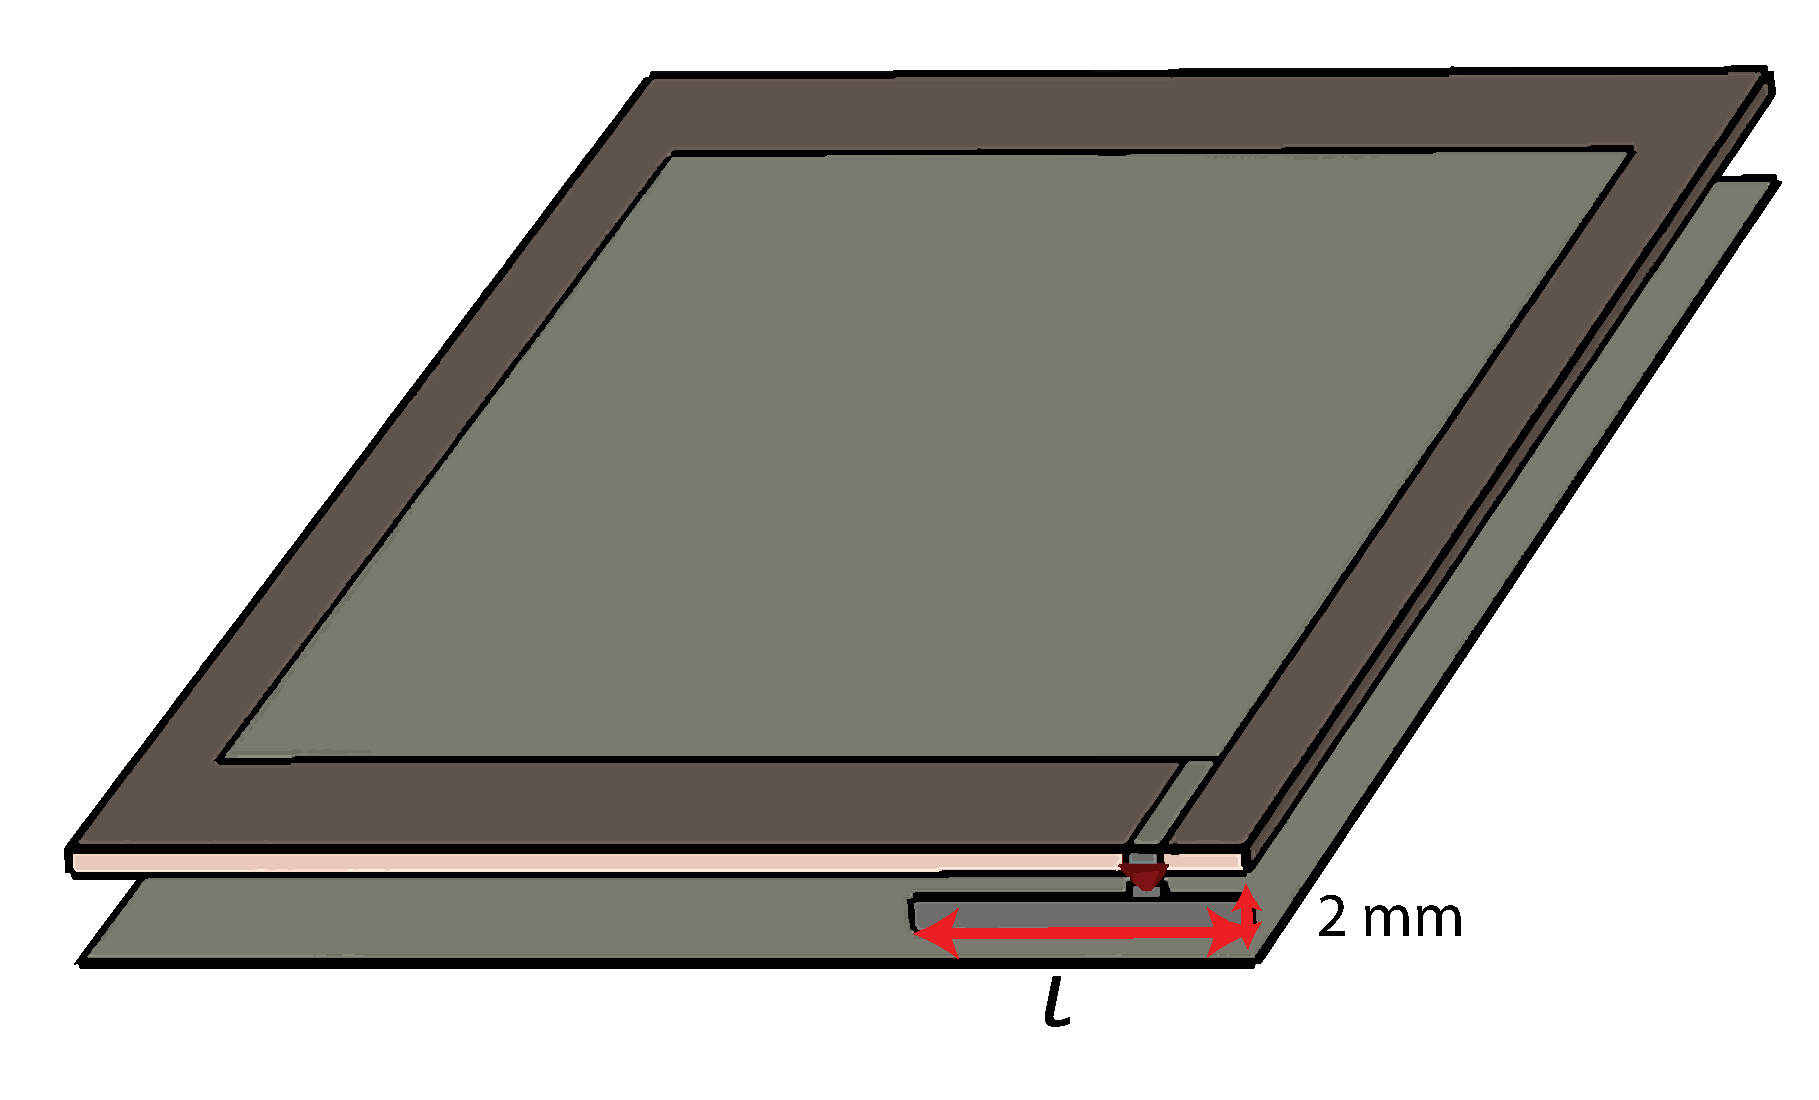
\includegraphics[width=\textwidth]{img/ant_length_short.eps}
        \caption{Antenna located on the top of the phone.}
        \label{fig:ant_length_short}
    \end{subfigure}
    \caption{Models used to test the effect of antenna's length.}
    \label{fig:ant_length_model}
\end{figure}

Figure \ref{fig:ant_length_result} shows the effect of antenna length with five different values in both cases. It is clear that especially in the low band, none of these antennas is suitable. Anyhow, few observations can be made from these simulations. Looking at Figure \ref{fig:ant_length_long_res} reveals that resonance of the longest antenna is not the strongest in the lowest frequencies. Instead, it is weakest and shorter antennas are better matched near the low band. Shortest tested antenna, having length of $20\,\milli\meter$, has the most promising performance in the high band.

Effects of antenna's length are quite similar, if antenna is placed on the top of the phone, like Figure \ref{fig:ant_length_short_res} presents. Again, none of the tested lengths fits for the low band, but this time the length does not make as clear difference. Each of the tested lengths has strong resonances near the low band at slightly different frequencies. Comparing the bandwidths of the lowest resonances, the antenna with length of $45\,\milli\meter$ has the widest bandwidth.

\begin{figure}[H]
    \centering
    \begin{subfigure}[b]{0.49\textwidth}
        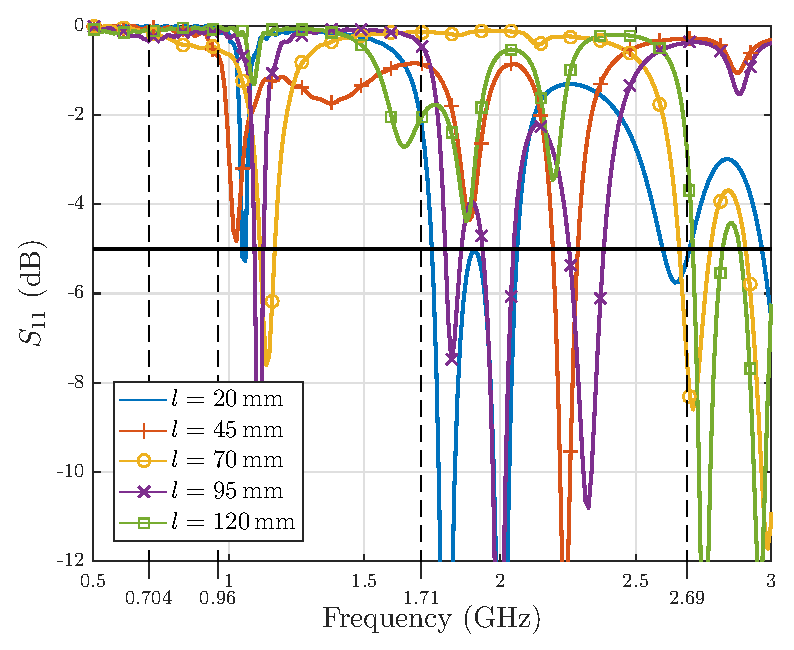
\includegraphics[width=\textwidth]{img/ant_length_long_res.eps}
        \caption{Antenna located on the side of the phone.}
        \label{fig:ant_length_long_res}
    \end{subfigure}
    \begin{subfigure}[b]{0.49\textwidth}
        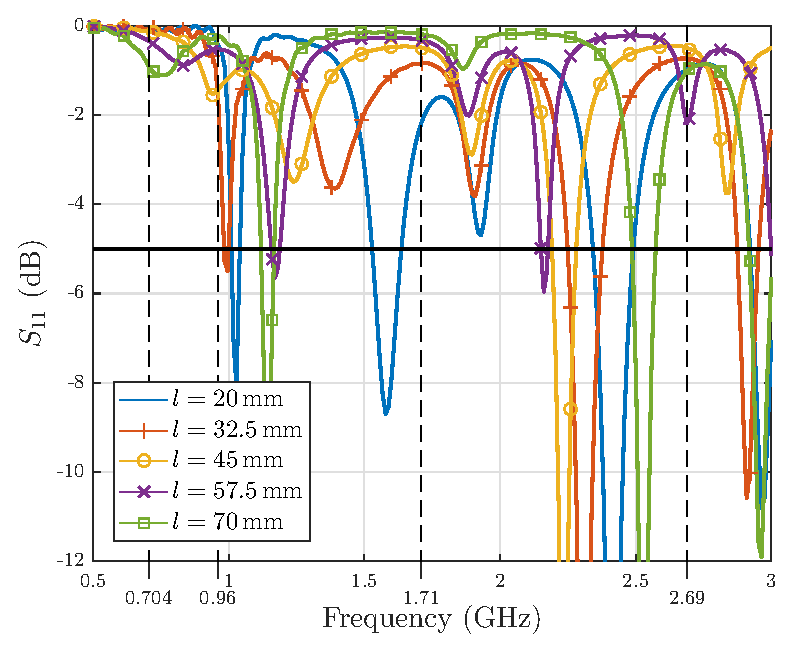
\includegraphics[width=\textwidth]{img/ant_length_short_res.eps}
        \caption{Antenna located on the top of the phone.}
        \label{fig:ant_length_short_res}
    \end{subfigure}
    \caption{The effect of antenna's length.}
    \label{fig:ant_length_result}
\end{figure}

The other matter affecting the size of an antenna besides length is its width. Impact of width is tested with the same structure that was used to test the effect of length, when the antenna is placed on the top of the phone. Antenna's length was also $70\,\milli\meter$ in this case. As Figure \ref{fig:width_res} presents, the effect of the width is quite minimal. Wider element gives a little bit better bandwidth in the both desired operational bands, but difference is not significant. Nevertheless the similarity of the results, larger bandwidth is more achievable with wider elements. Only it must be remembered, that the space for antennas is very limited on the sides of the phone, and thus, antennas cannot be much wider.

\begin{figure}[H]
    \centering
    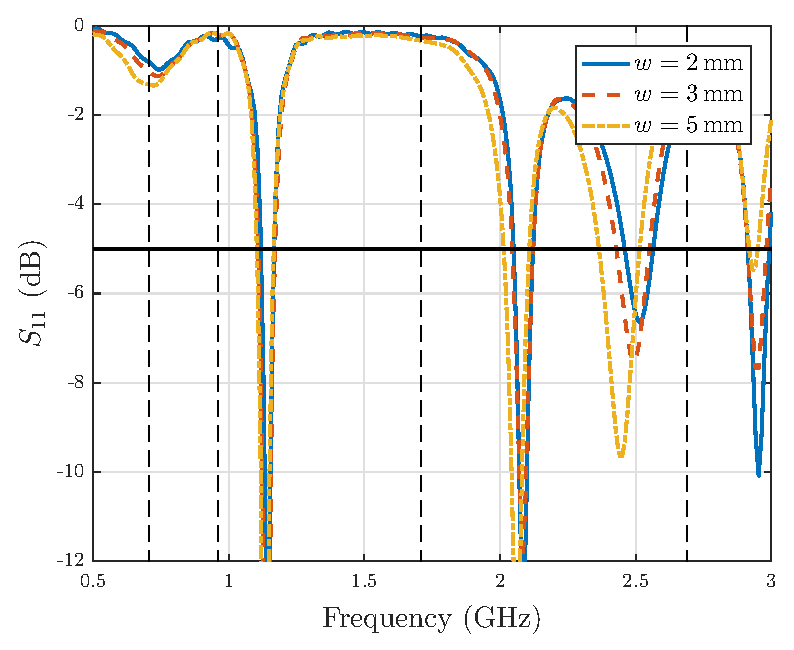
\includegraphics[width=0.5\textwidth]{img/width_res.eps}
    \caption{Effect of the width of an antenna.}
    \label{fig:width_res}
\end{figure}

Besides the size of antenna, another interesting parameter is the location of the feed. This is tested with the same structure that was used to test the impact of the metallic back cover except for the small block on the corner, shown in Figure \ref{fig:metal_cover} earlier. Feeds are located in two ways: either on the long or the short side, like in Figures \ref{fig:ant_length_long} and \ref{fig:ant_length_short}, respectively. Feed is placed between the antenna and the ground plane, or the display in this case, and four different locations are tested on each side. The first position is in the corner of the ground plane, and the last is in the center of it. Between these are two positions at equal distances, denoted as ground 1/3 and ground 2/3.

Figures \ref{fig:feed_pos_side_res} and \ref{fig:feed_pos_top_res} show the simulation results for feed on the long side and feed on top, respectively. Both of these graphs yield the same conclusion: for the low band, feed provides better bandwidth when located at the corner of the ground plane. For the high band, feed location is the most promising when it is shifted away from the corner, and is located on the top side of the phone.

\begin{figure}[H]
    \centering
    \begin{subfigure}[b]{0.49\textwidth}
        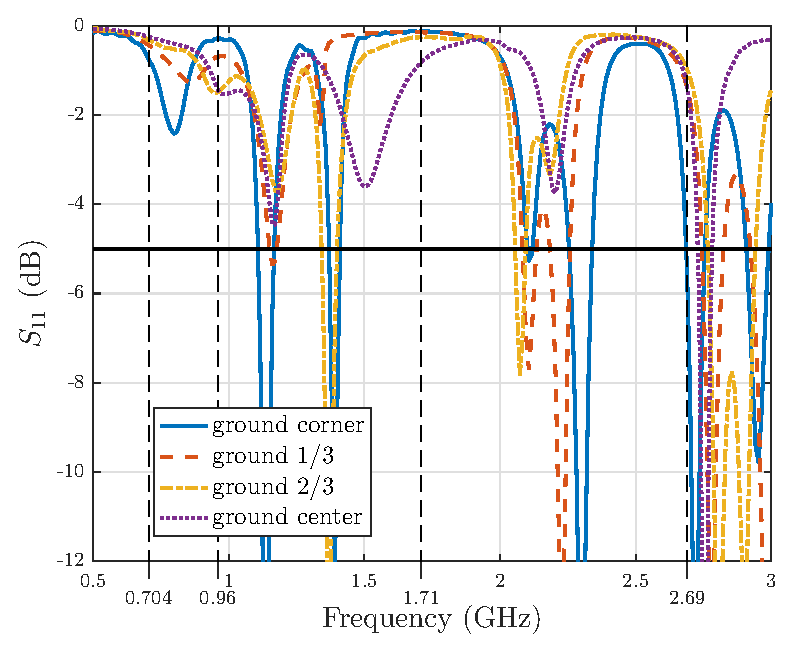
\includegraphics[width=\textwidth]{img/feed_pos_side_res.eps}
        \caption{Antenna located on the side of the phone.}
        \label{fig:feed_pos_side_res}
    \end{subfigure}
    \begin{subfigure}[b]{0.49\textwidth}
        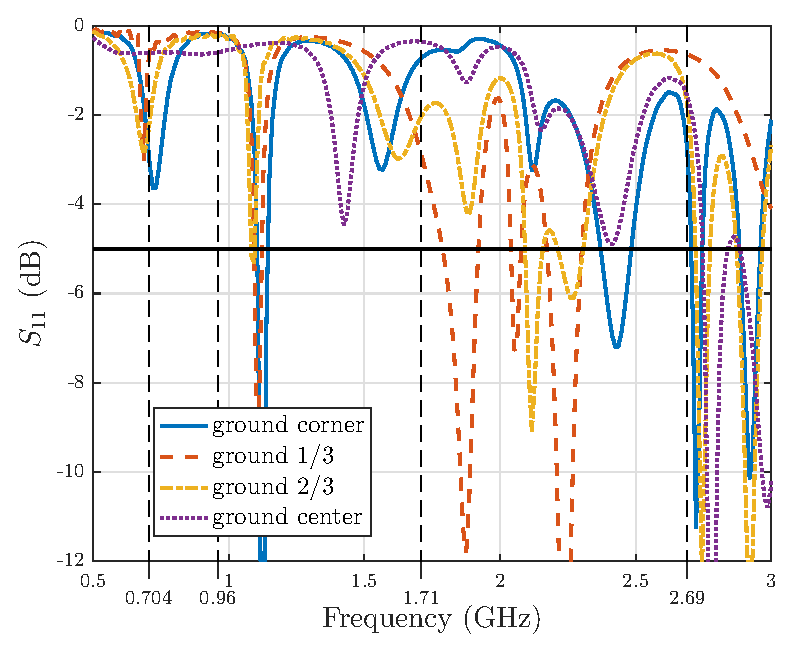
\includegraphics[width=\textwidth]{img/feed_pos_top_res.eps}
        \caption{Antenna located on the top of the phone.}
        \label{fig:feed_pos_top_res}
    \end{subfigure}
    \caption{The effect of the location of the feed.}
    \label{fig:feed_effect}
\end{figure}

Positioning the antenna is as well worth testing. In this test, a $70\,\milli\meter$ long sheet is used, and it is bent over a corner to form an L-shaped structure. The total length of this element is the same as was one option in testing the effect of length, to have comparability. Antenna is positioned in one corner of the phone in four different ways presented in Table \ref{tab:l_structures}. The lengths on each side are kept the same, and positioning is changed by rotating the element. Feed is placed in the corner of the ground plane, and is oriented along either the long or the short side. Figure \ref{fig:l_shape_model} illustrates the model. In this illustration feed is placed on the long side of the phone.

Results are presented in Figure \ref{fig:l_shape_res}. The nature of each curve is very similar, especially other structures but 1, that are almost identical below ca. $2.3\,\giga\hertz$. As these three structures have quite strong resonance above $1\,\giga\hertz$, the blue curve of structure 1 is showing promising wideband performance. Although the good band is just above the low band, where performance of each setup is very weak, this test shows that wide band matching might be achievable with L-shaped elements in the corners.

\begin{table}[H]
    \centering
    \caption{Antenna parameters used while testing L-shaped antenna structures.}
    \label{tab:l_structures}
    \begin{tabular}{|M{0.22\textwidth}|M{0.22\textwidth}|M{0.22\textwidth}|M{0.22\textwidth}|}
        \hline
        \textbf{Antenna structure} & \textbf{Antenna length on the long side ($l_1$)} & \textbf{Antenna length on the short side ($l_2$)} & \textbf{Feed orientation}\\
        \hline
         Structure A & $50\,\milli\meter$ & $20\,\milli\meter$ & On the long side\\
         \hline
         Structure B & $50\,\milli\meter$ & $20\,\milli\meter$ & On the short side\\
         \hline   
         Structure C & $20\,\milli\meter$ & $50\,\milli\meter$ & On the short side\\
         \hline
         Structure D & $20\,\milli\meter$ & $50\,\milli\meter$ & On the long side\\
         \hline
    \end{tabular}
\end{table}

\begin{figure}[H]
    \centering
    \begin{subfigure}[b]{0.49\textwidth}
        \includegraphics[width=\textwidth]{img/L_shape.eps}
        \caption{Model of L-shaped antenna.}
        \label{fig:l_shape_model}
    \end{subfigure}
    \begin{subfigure}[b]{0.49\textwidth}
        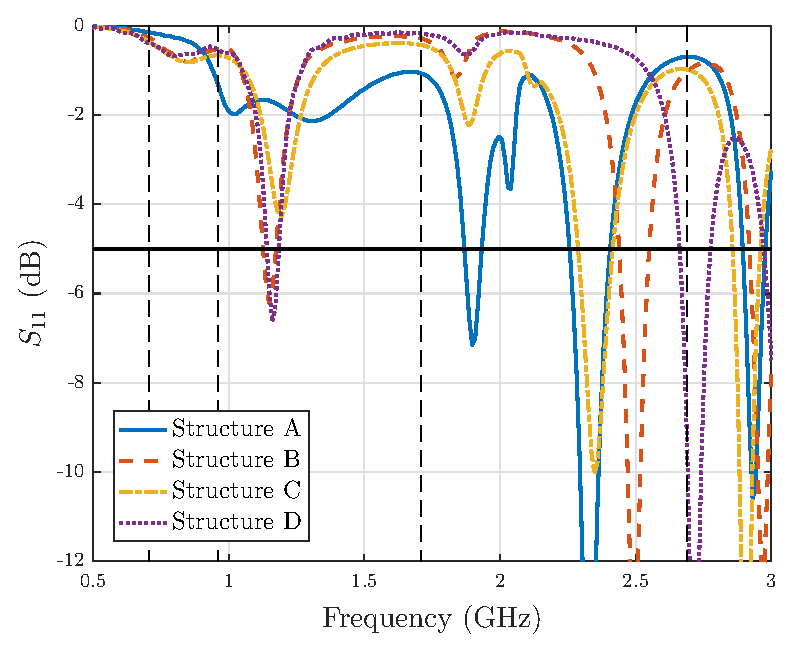
\includegraphics[width=\textwidth]{img/L_shape_res.eps}
        \caption{Results from simulations.}
        \label{fig:l_shape_res}
    \end{subfigure}
    \caption{Simulated L-shaped antennas.}
    \label{fig:l_shape}
\end{figure}

So far all investigated antennas have been either straight, rectangular sheets or L-shaped elements. Modifying the shape more might enable to excite different resonant modes. Figure \ref{fig:shape_models} shows six shapes of different complexity implemented on the top of the handset. All the tested structures are fed from the same corner of the ground plane. To make it clear, the antennas of shapes 4, 5, and 6 (\Cref{fig:shape4,fig:shape5,fig:shape6}, respectively) are $0.5\,\milli\meter$ apart from the cover.

\begin{figure}[H]
    \centering
    \begin{subfigure}[b]{0.3\textwidth}
        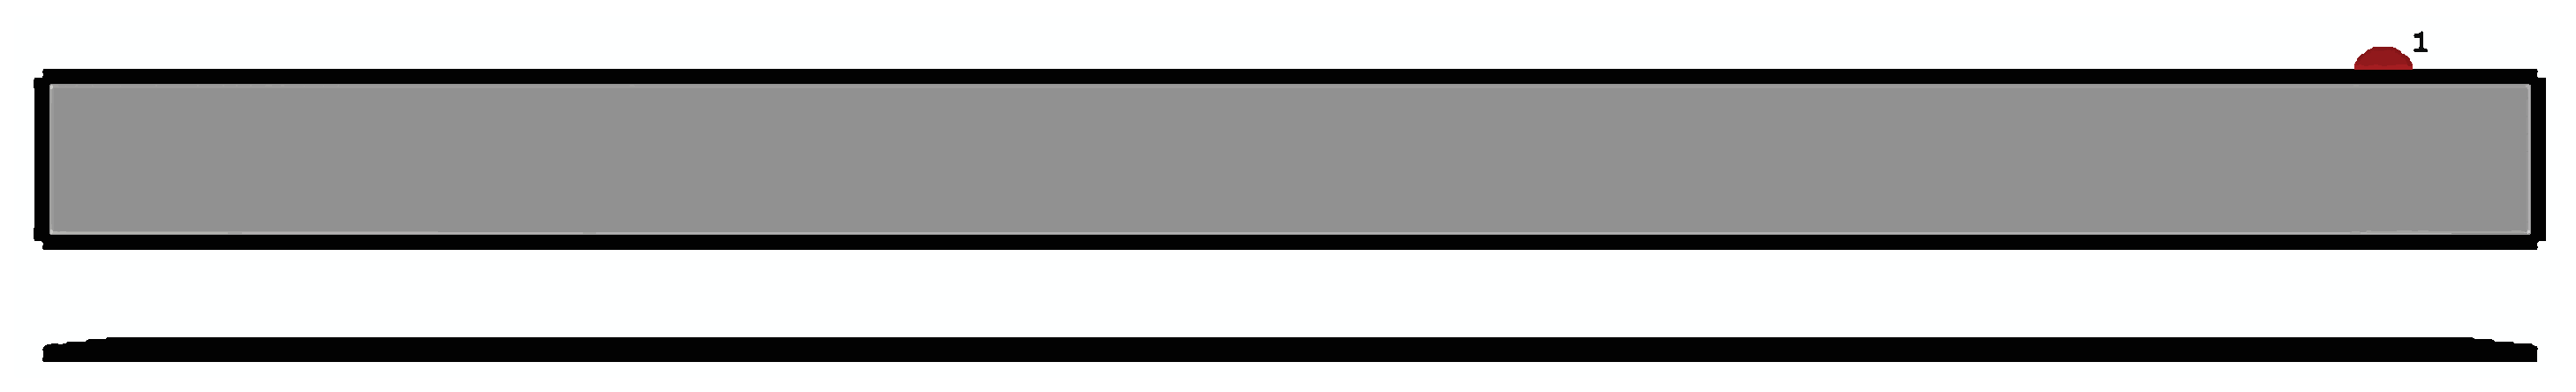
\includegraphics[width=\textwidth]{img/shape1.eps}
        \caption{Shape 1.}
        \label{fig:shape1}
    \end{subfigure}
    \begin{subfigure}[b]{0.3\textwidth}
        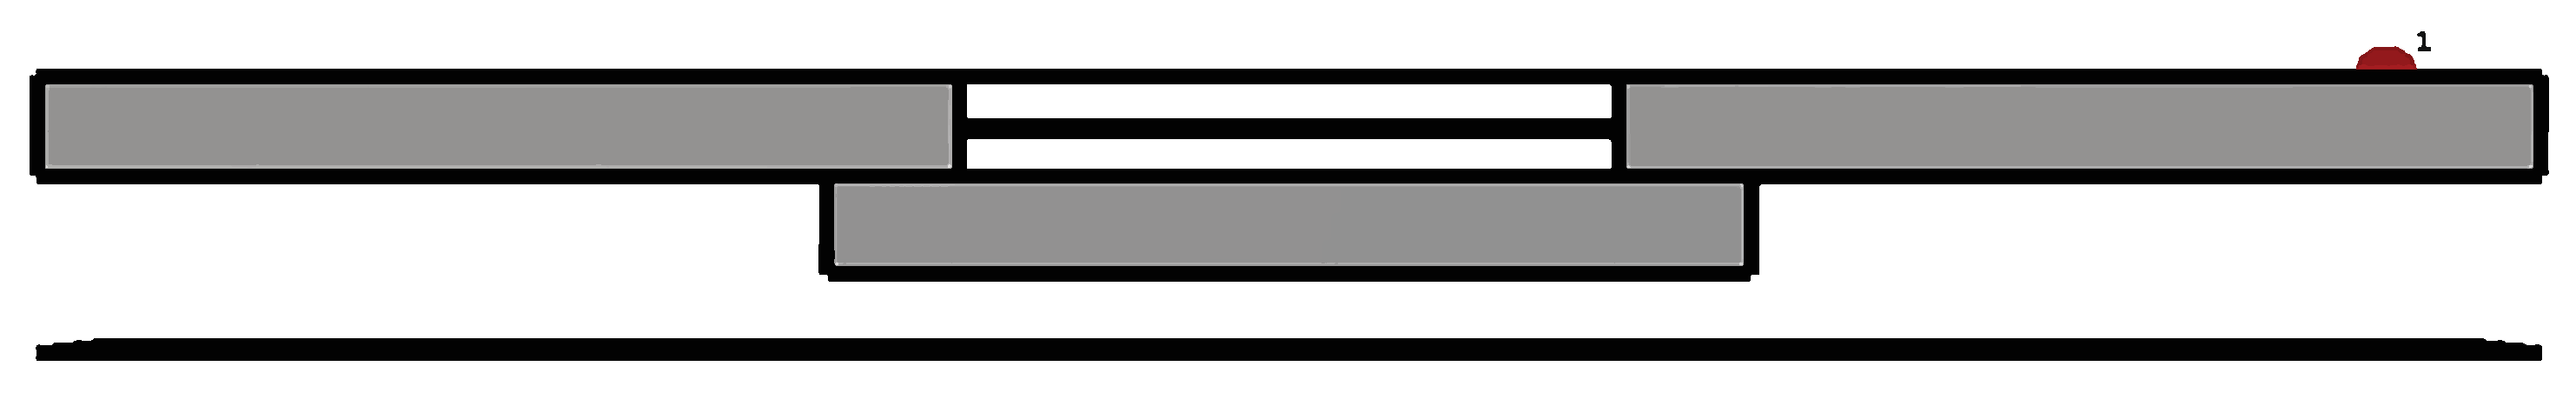
\includegraphics[width=\textwidth]{img/shape2.eps}
        \caption{Shape 2.}
        \label{fig:shape2}
    \end{subfigure}
    \begin{subfigure}[b]{0.3\textwidth}
        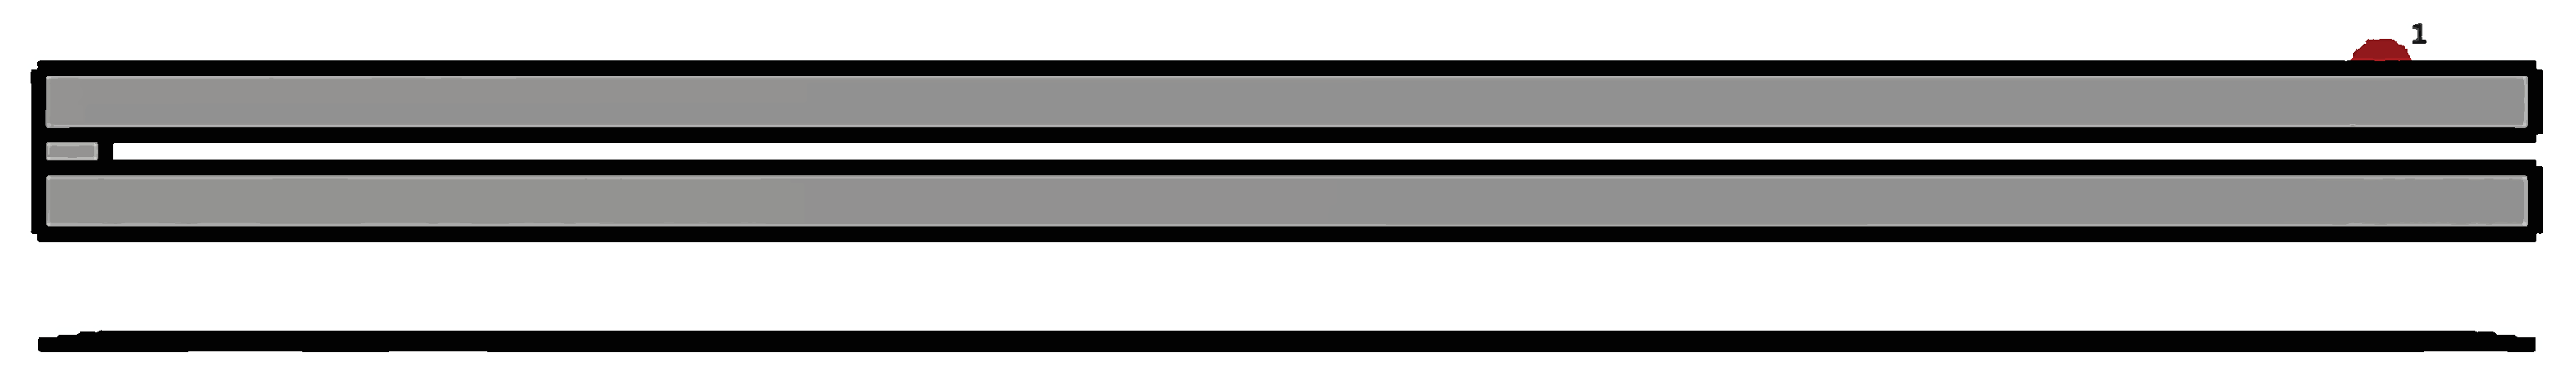
\includegraphics[width=\textwidth]{img/shape3.eps}
        \caption{Shape 3.}
        \label{fig:shape3}
    \end{subfigure}
    
    \begin{subfigure}[b]{0.3\textwidth}
        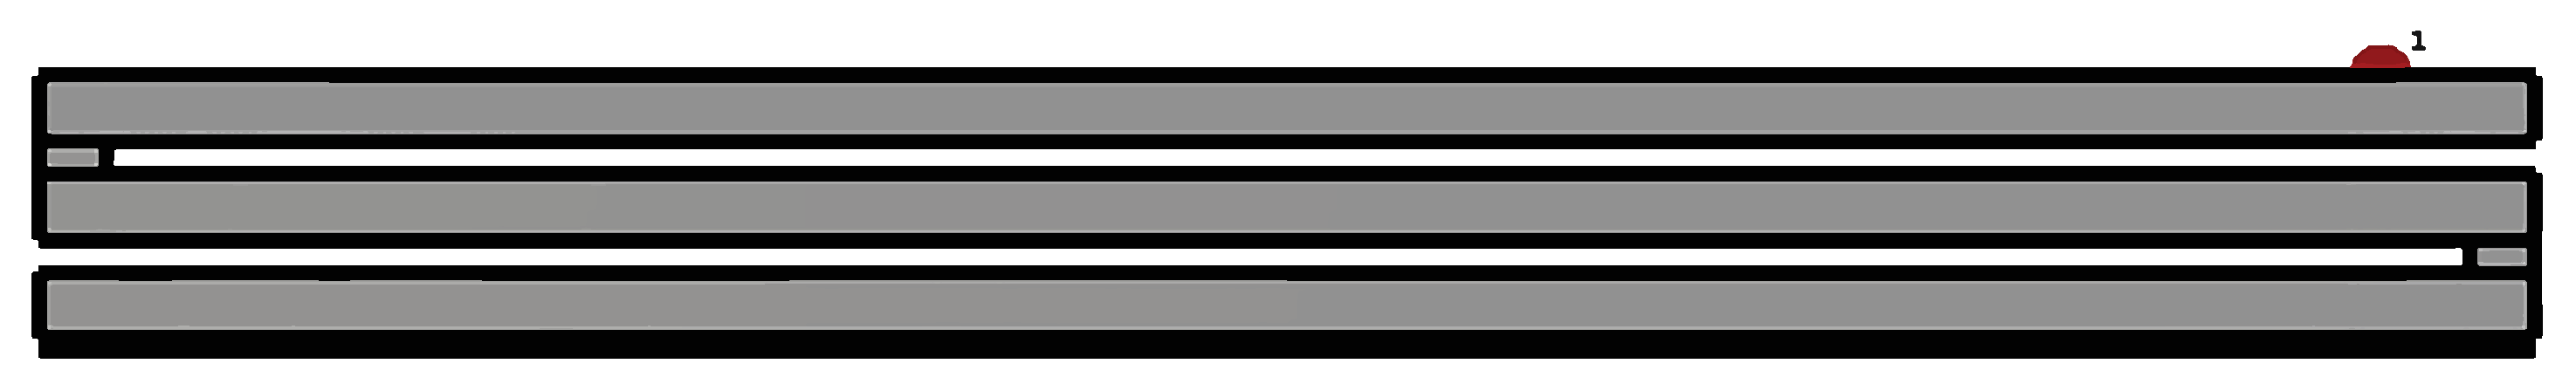
\includegraphics[width=\textwidth]{img/shape4.eps}
        \caption{Shape 4.}
        \label{fig:shape4}
    \end{subfigure}
    \begin{subfigure}[b]{0.3\textwidth}
        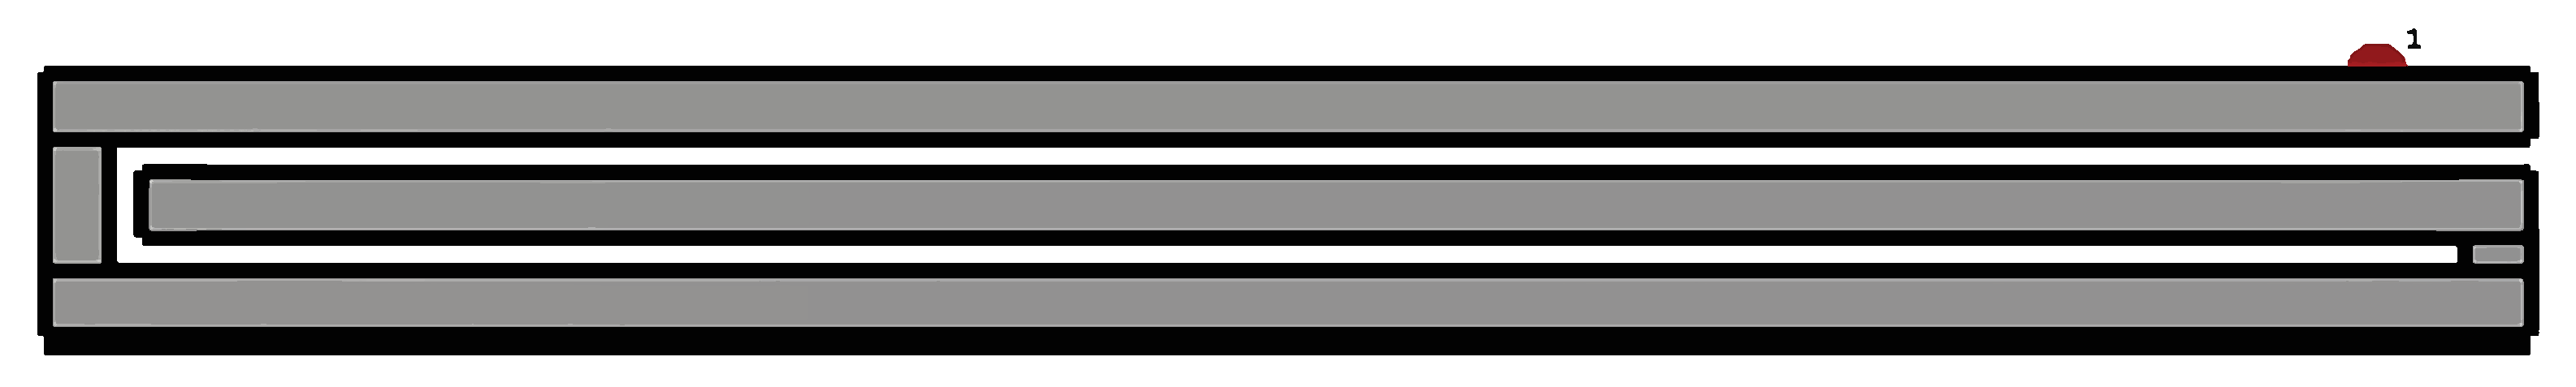
\includegraphics[width=\textwidth]{img/shape5.eps}
        \caption{Shape 5.}
        \label{fig:shape5}
    \end{subfigure}
    \begin{subfigure}[b]{0.3\textwidth}
        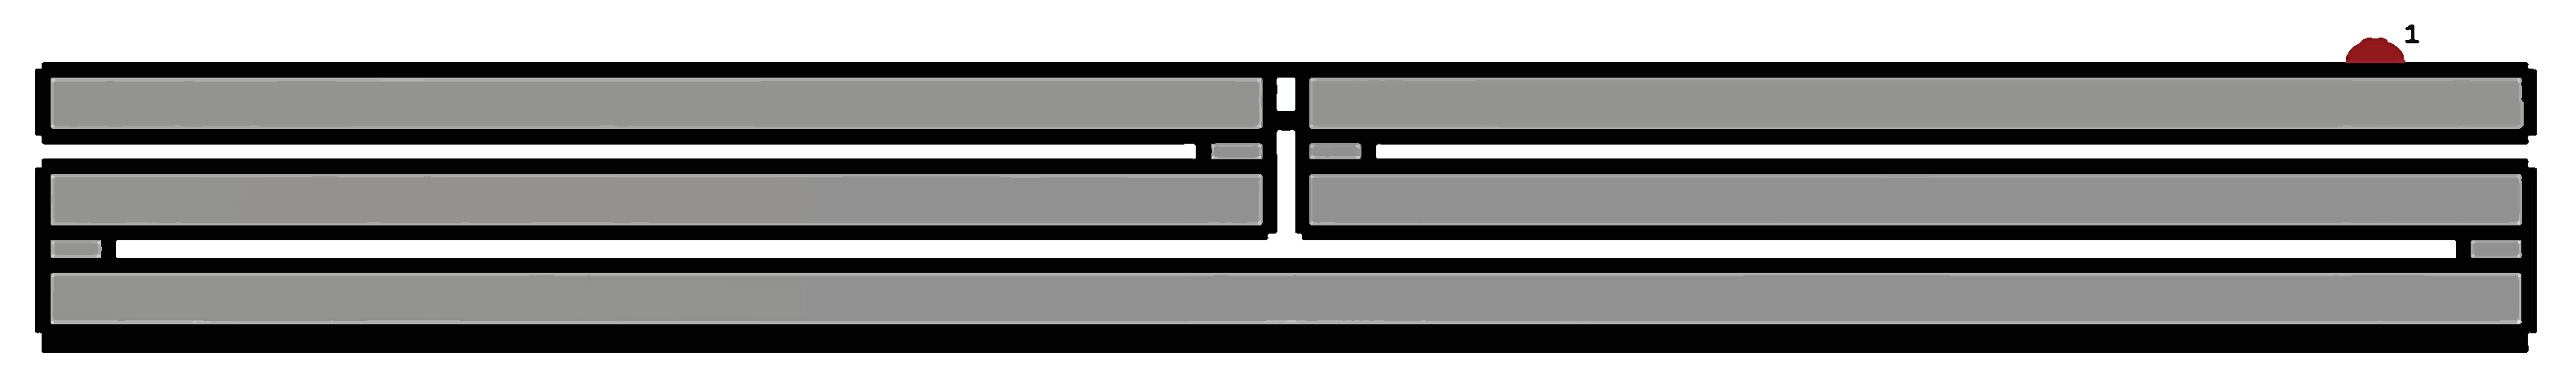
\includegraphics[width=\textwidth]{img/shape6.eps}
        \caption{Shape 6.}
        \label{fig:shape6}
    \end{subfigure}
    \caption{Different shapes for antenna located at the end of the phone.}
    \label{fig:shape_models}
\end{figure}

Results can be seen in Figure \ref{fig:shape}. For the low band, shape 4 has the best matching and quite good bandwidth. The two most simple shapes, 1 and 2, produce almost identical results, and in the lowest frequencies they are somewhat wideband, though the matching level is poor. These simpler structures also operate better in the high band than other tested antennas.

\begin{figure}[H]
    \centering
    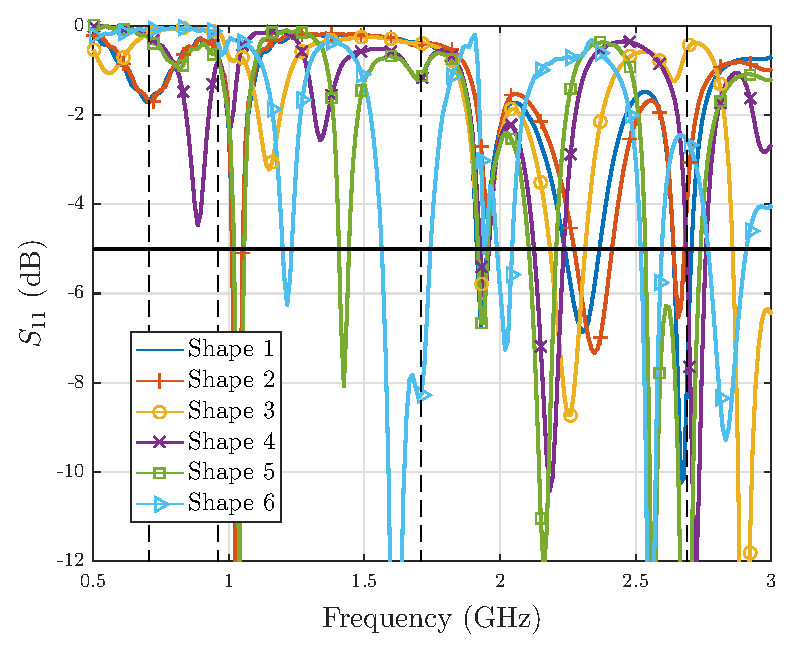
\includegraphics[width=0.5\textwidth]{img/shape.eps}
    \caption{Effect of different antenna shapes. Antennas are located at the end of a phone.}
    \label{fig:shape}
\end{figure}

%\subsubsection*{lol}

As was shown in earlier Figure \ref{fig:metal_rim}, possible locations for antennas are above and below the display of the phone. Therefore, an antenna element is placed in that area, illustrated in Figure \ref{fig:front_model}, and compared to a similar element located on the top of the phone, like shown in Figure \ref{fig:shape1}. It can be seen from Figure \ref{fig:front_res} that the difference between these two locations is minimal. The shapes of the responses are nearly identical in the low frequencies, and they follow the same pattern in the higher band. Matching levels at the low band are bad, but the bandwidth is quite wide. In the high band, the element on the front gives good matching on two sub-bands, and is promising in the rest of the band also.

\begin{figure}[H]
    \centering
    \begin{subfigure}[b]{0.49\textwidth}
        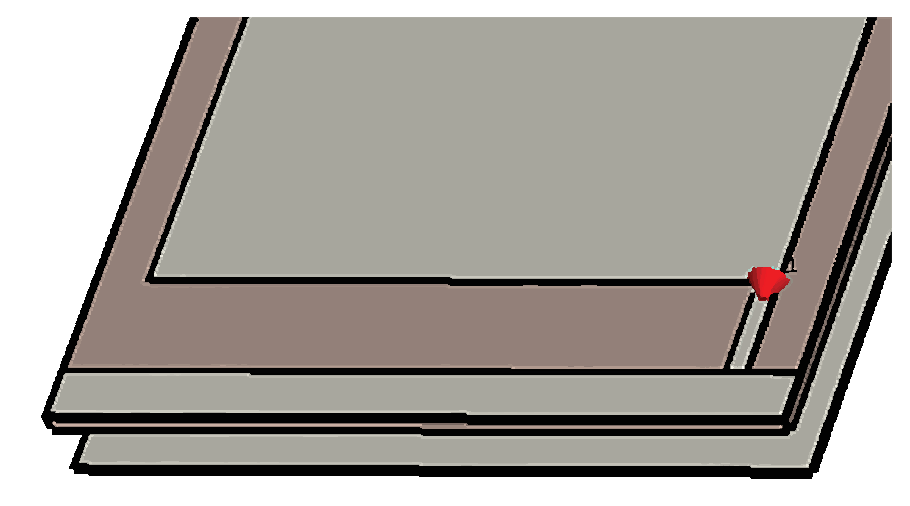
\includegraphics[width=\textwidth]{img/front.eps}
        \caption{Model of frontside antenna element.}
        \label{fig:front_model}
    \end{subfigure}
    \begin{subfigure}[b]{0.49\textwidth}
        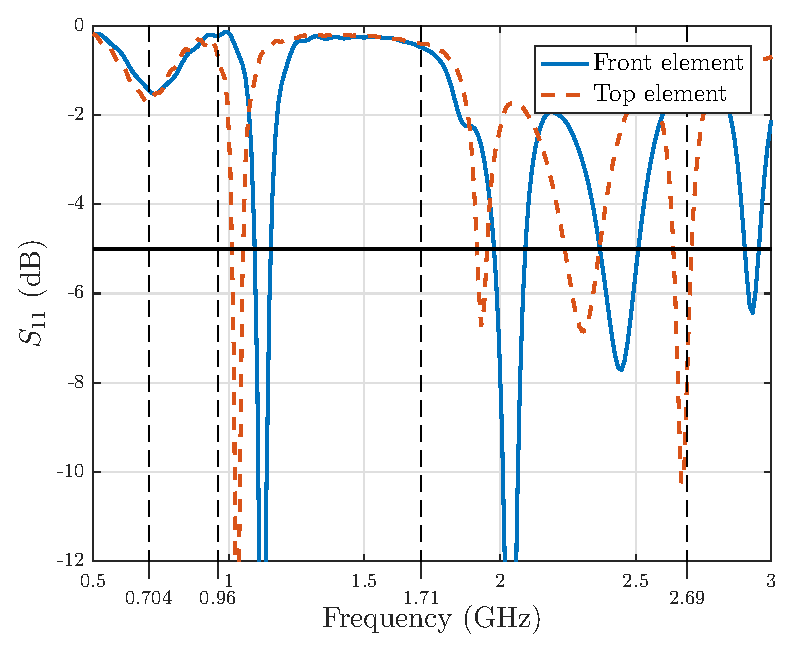
\includegraphics[width=\textwidth]{img/front_res.eps}
        \caption{Results from simulations.}
        \label{fig:front_res}
    \end{subfigure}
    \caption{Antenna element on the front side of the phone.}
    \label{fig:front_elem}
\end{figure}

In addition to straight sheets, slots can be added to elements to introduce new wave modes. This test has the same antenna as presented in Figure \ref{fig:metal_cover}, with one or two slots on the sides. The first slot on the long side, at $20\,\milli\meter$ from the end, and second is on the short side at the same distance from the end of the element. Both slots are $2\,\milli\meter$ wide.

Adding one slot creates strong and very narrow peak at low band, as can be seen from Figure \ref{fig:slot_res}. Second slot gives slightly wider bandwidth, but decreases matching level compared to zero or one slot.

\begin{figure}[H]
    \centering
    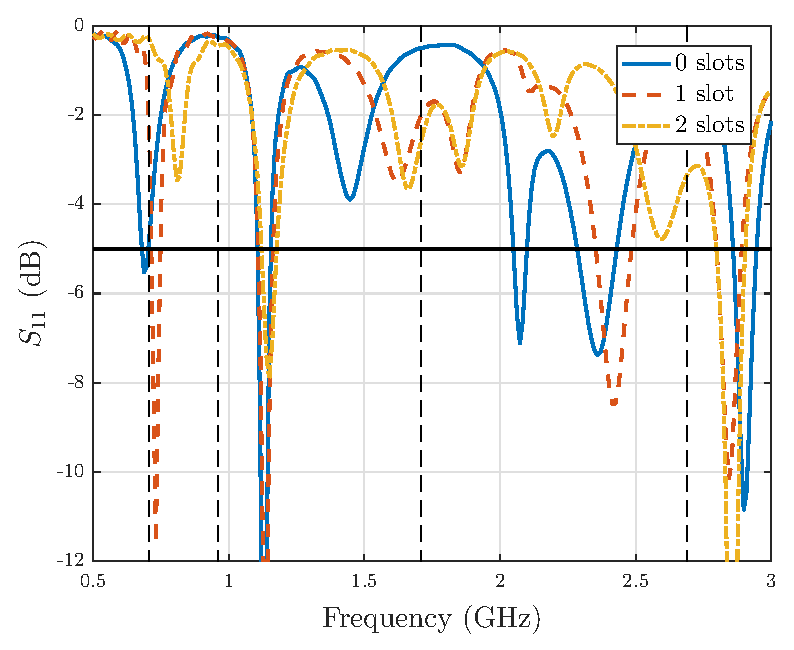
\includegraphics[width=0.5\textwidth]{img/slot_res.eps}
    \caption{Effect of slots in the antenna element.}
    \label{fig:slot_res}
\end{figure}

Last thing to investigate is the effect of ground plane. So far phone's display has been used as a ground plane, but since the back cover is also large metallic plate, that could be used as well as a ground. The test setup is the same as was used to the effect of metal cover, shown in Figure \ref{fig:metal_cover}. Only feed is moved between the iterations. Figure \ref{fig:ground_plane} shows the impact. When feed is moved to locate between the back cover and antenna element, the response is much smoother, and has wider bandwidths and better matching levels. One possible explanation for this behavior might rely on the sizes of the two planes. When display is used as a ground plane, the larger back cover interacts with the EM-fields stronger and therefore is more harmful for the antennas. If feed is grounded to the back cover, then the disturbing element is smaller and negative effects are not as strong.

\begin{figure}[H]
    \centering
    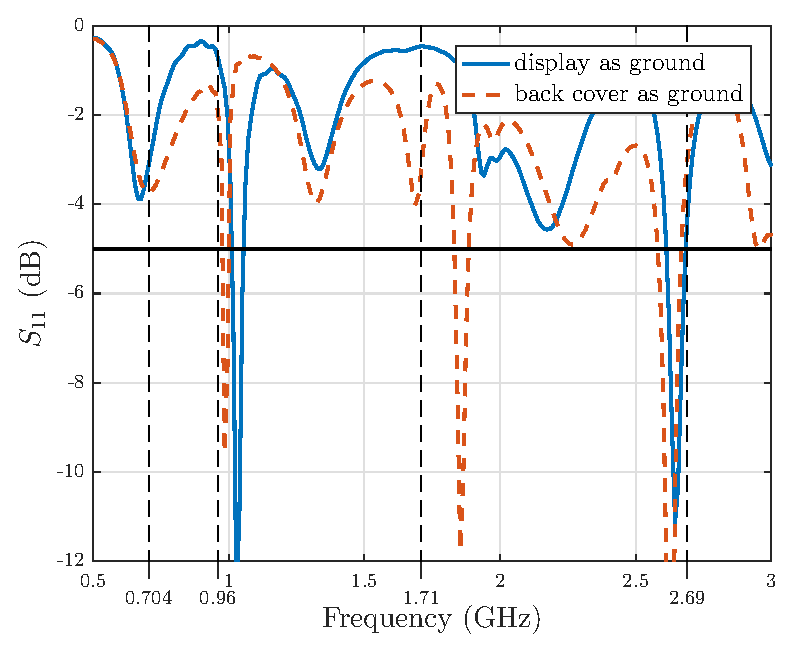
\includegraphics[width=0.5\textwidth]{img/ground_vs_display.eps}
    \caption{Effect of using display or back cover as ground plane.}
    \label{fig:ground_plane}
\end{figure}

The conclusions made from all these presented simulation results are collected and summarized in Table \ref{tab:dimension_summary} below. 

\begin{table}[H]
    \centering
    \caption{Summary of how changing dimensions affect antenna's performance.}
    \label{tab:dimension_summary}
    \begin{tabular}{|p{0.28\textwidth}|p{0.65\textwidth}|}
        \hline
        \textbf{Changed parameter} & \textbf{Impact on antenna's performance} \\
        \hline
        Element length on the side of the phone & Resonance frequencies variate and longer elements tend to lower the frequency.\\
        \hline
        Element length on the end of the phone & Resonance frequencies variate and longer elements tend to lower the frequency.\\
        \hline
        Element on the front side of the phone & Adding element improves matching levels.\\
        \hline
        Element width & Wider element slightly increases bandwidth.\\
        \hline
        Location of the feed & Feed close to a corner of the display gives wider band, although resonance is smoother if feed is in the center.\\
        \hline
        Ground plane & Using back cover as a ground plane instead of the display gives wider bandwidths and more resonating frequencies.\\
        \hline
        Shape of the element & The more complex the element is, the more it resonates. Large loops increase bandwidth. Elements bended over the corner (L-shaped) even resonances and improve matching levels.\\
        \hline
        Slots & Slots in the element on the long side narrow bands and on the short side decrease matching levels.\\
        \hline
    \end{tabular}
\end{table} 

\subsubsection{Conceptualizing the main antenna}
\label{sec:conceptualizing}

The basic concept of the main antenna was created on the ground of the findings of the dimension study. The main antenna should be located mainly on the short side of the phone and construct of simple shapes. Its elements should be rather short and they can be banded over the corner of the phone. Also, it was noticed that slots might improve bandwidth, and thus, could be used to cover both defined frequency sets. 

The main antenna was decided to consist of three elements. Two of them were L-shaped strips bending over the corners of the phone. The last element was a U-shaped sheet on the frontside of the phone, above the display. Back cover was used as a ground plane since it was earlier found to be better choice than the display. At first, this structure was single-fed, and the feed was connected between the U-shaped element and the ground plane. Figure \ref{fig:main_concept} shows the structure of this concept, and Figure \ref{fig:main_location} gives a better view of the location of the antenna.

\begin{figure}[H]
    \centering
    \begin{subfigure}[b]{0.49\textwidth}
        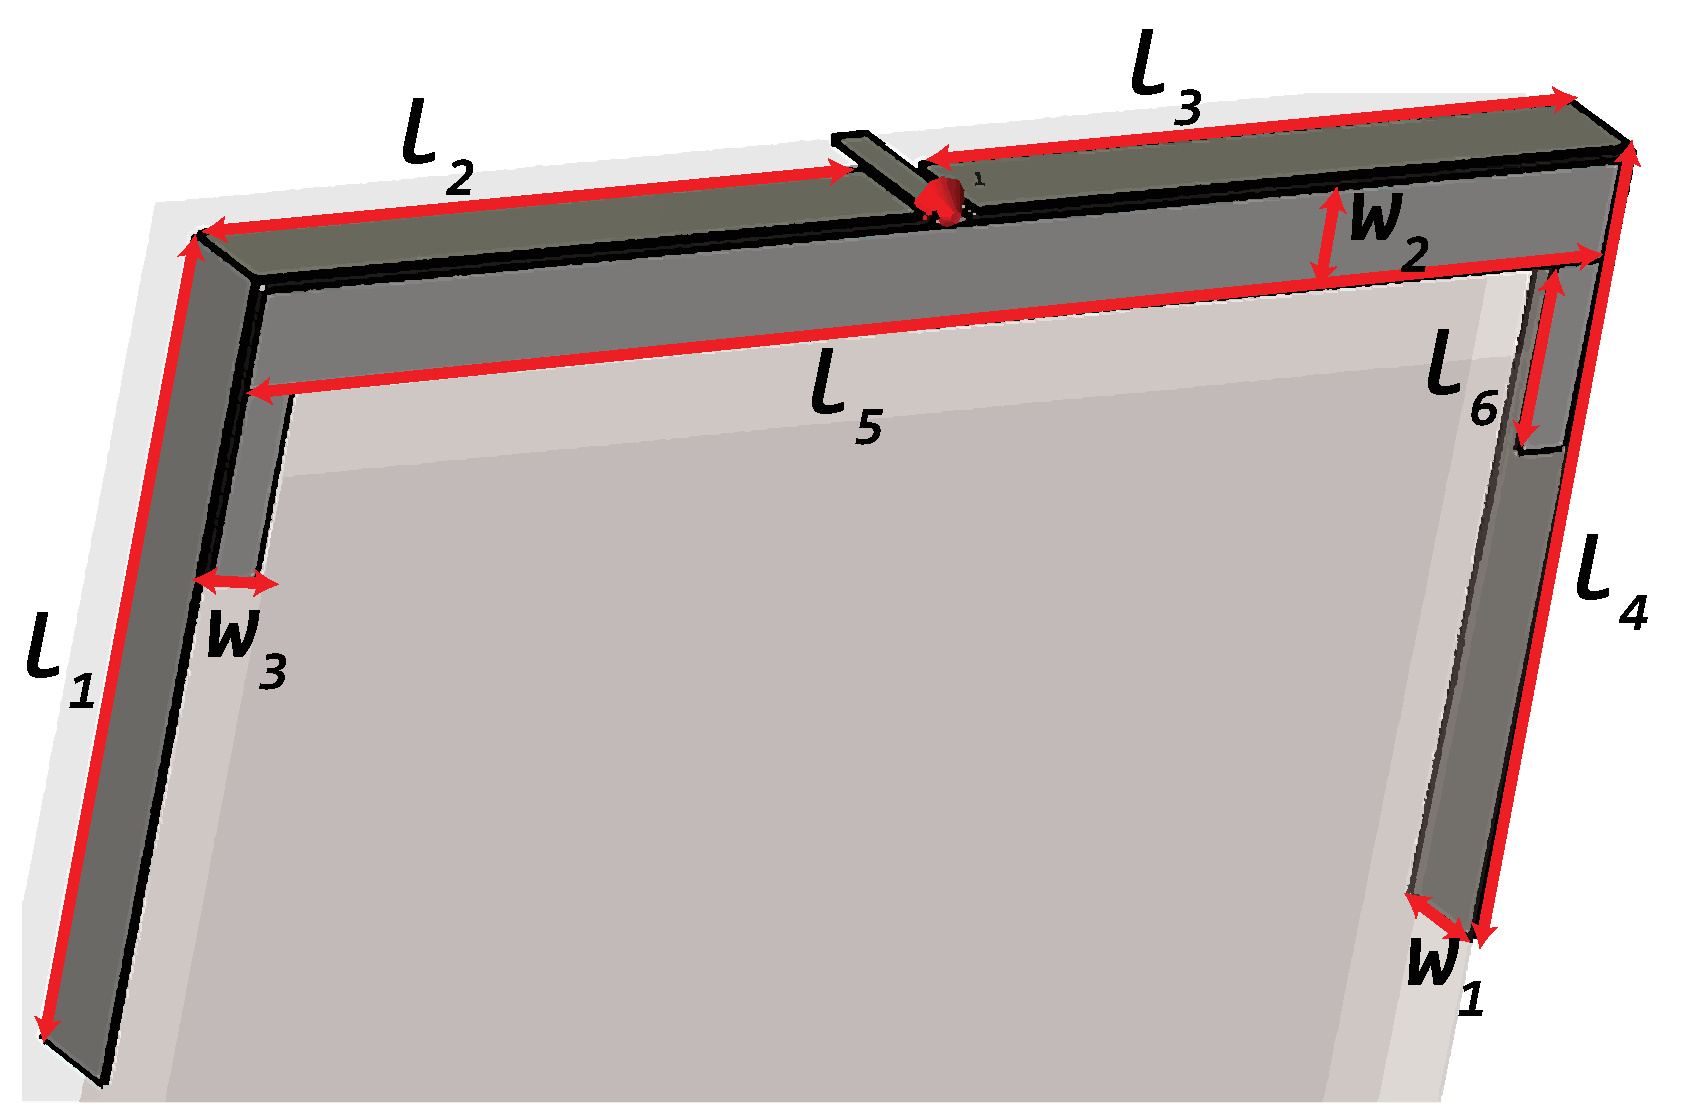
\includegraphics[width=\textwidth]{img/main_concept.eps}
        \caption{Structure.}
        \label{fig:main_concept}
    \end{subfigure}
    \begin{subfigure}[b]{0.49\textwidth}
        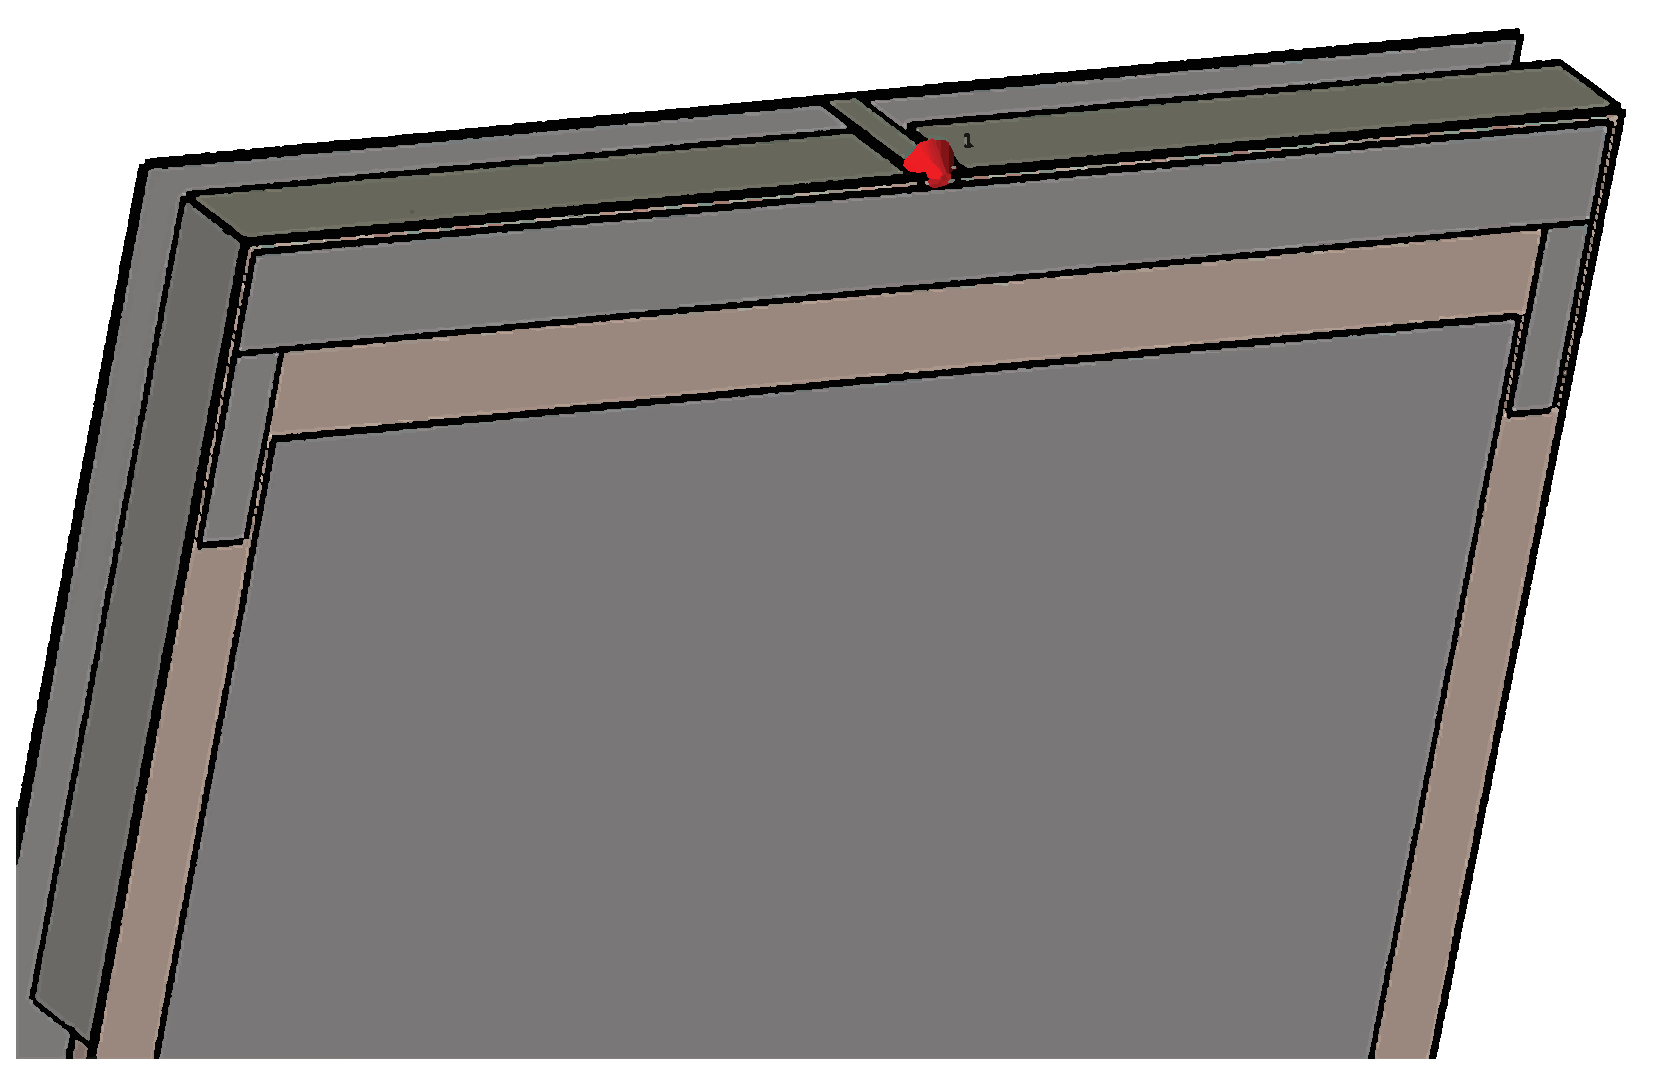
\includegraphics[width=\textwidth]{img/main_location.eps}
        \caption{Location.}
        \label{fig:main_location}
    \end{subfigure}
    \caption{Concept for the main antenna.}
    \label{fig:main_antenna1}
\end{figure}

The underlying idea of this structure is to have strong mutual coupling between the three antenna elements, which would hopefully improve the operational bandwidth of the system. Elements were placed very close to each others to have better coupling effect the gap between the U-shaped and the L-shaped elements being only $0.5\,\milli\meter$. The same gap width was also used between the barbs of the U-antenna and the display, and to separate the L-elements from the feed pin.

This concept was improved and modified further via a number of simulation iterations. Between the different simulation rounds, the structures and dimensions were modified the same way as it was done in the preliminary study. The main values of interest are illustrated in Figure \ref{fig:main_concept}, and their initial values can be seen from Table \ref{tab:initial_concept}. Besides these parameters, also location of the feed and the gaps between the elements were tested. 
\begin{table}[H]
    \centering
    \caption{Initial values for the main antenna concept.}
    \label{tab:initial_concept}
    \begin{tabular}{|c|c|}
        \hline
        \textbf{Dimension} & \textbf{Value [$\milli\meter$]} \\
        \hline
        $l_1$ & 40\\
        \hline
        $l_2$ & 36.5\\
        \hline
        $l_3$ & 36.5\\
        \hline
        $l_4$ & 40\\
        \hline
        $l_5$ & 75\\
        \hline
        $l_6$ & 9.5\\
        \hline
        $w_1$ & 5\\
        \hline
        $w_2$ & 5\\
        \hline
        $w_3$ & 2.55\\
        \hline
    \end{tabular}
\end{table}

Already the first simulation showed very promising results, as can be seen from Figure \ref{fig:concept_ini}. Shape of the response in the low band is exactly what was desired: wide and smooth. However, the results were not all positive. The matching level in the low band is only about $-2\,\db$, and the high band is terrible. The first conclusion of this result is that either symmetric structure is not optimal or the dimensions of the different parts are not what they are supposed to be.
\begin{figure}[H]
    \centering
    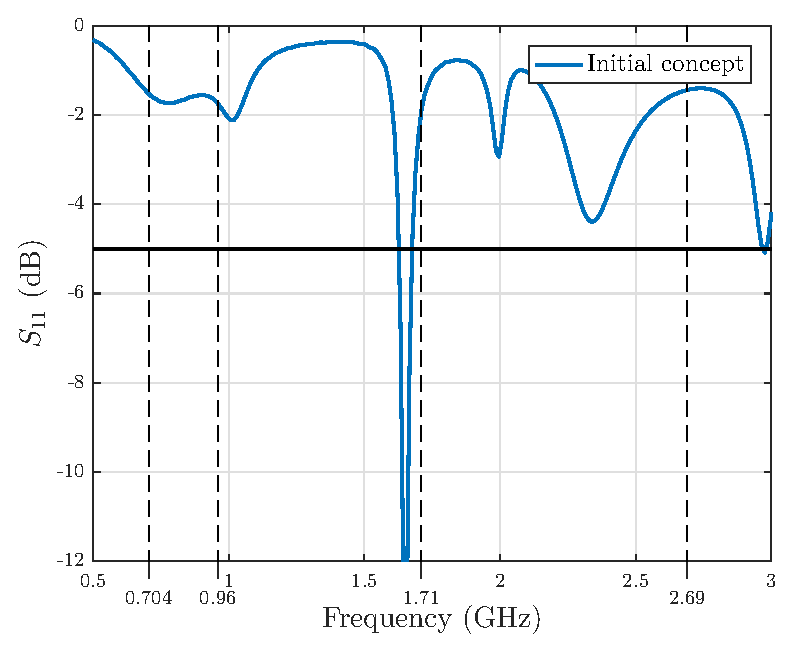
\includegraphics[width=0.5\textwidth]{img/concept_ini.eps}
    \caption{Concept tested with the initial values.}
    \label{fig:concept_ini}
\end{figure}

The structure was first modified by changing the dimensional parameters. For now, the system was still kept symmetric to preserve simplicity. The changed dimensions were the lengths of the metal sheets beside the display ($l_6$), lengths of the antennas on the sides of the phone ($l_1$, $l_4$) and the width of all the side antennas ($w_1$).  All these parameters were tested separately by the same principles used in the preliminary study, but in more detail. As the observations were similar to the ones preliminary study, only the best results are presented. Table \ref{tab:concept2} lists the best values for these parameters found in the three cases. Cases A, B, and C refer to changing $l_6$, $l_1$ and $l_4$, or $w_1$, respectively. 
\begin{table}[H]
    \centering
    \caption{Tested dimensions. All values are in millimeters.}
    \label{tab:concept2}
    \begin{tabular}{|c|c|c|c|c|}
        \hline
        \textbf{Dimension} & \textbf{Initial} & \textbf{Case A} & \textbf{Case B} & \textbf{Case C}\\
        \hline
        $l_1$ & 40 & 40 & 26 & 26\\
        \hline
        $l_4$ & 40 & 40 & 26 & 26\\
        \hline
        $l_6$ & 9.5 & 2.5 & 2.5 & 2.5\\
        \hline
        $w_1$ & 5 & 5 & 5 & 4\\
        \hline
    \end{tabular}
\end{table}

The values of tested dimensions ranged from both larger than the initial value to smaller than that. The Table \ref{tab:concept2} above shows that the best values are smaller than the initial one for all parameters. The results especially for $l_1$, $l_4$, and $l_6$ agree with the findings from the pre-study: better low band is achieved with smaller element on the side. $w_6$ however is smaller than the initial width but provides better results, even though the pre-study showed the opposite. In this case, as it was in the pre-study, the variations in the matching level between the different widths were marginal, but the chosen $4\,\milli\meter$ provided the smoothest response in the low band.

Figure \ref{fig:concept2} shows the best results of the three test cases compared with the initial situation. It can be seen clearly, that each modification have improved system's performance in the low band. Although the focus is in the low band, the high band should not be forgotten. In that area, the overall performance did not improve as the structure was modified. 
\begin{figure}[H]
    \centering
    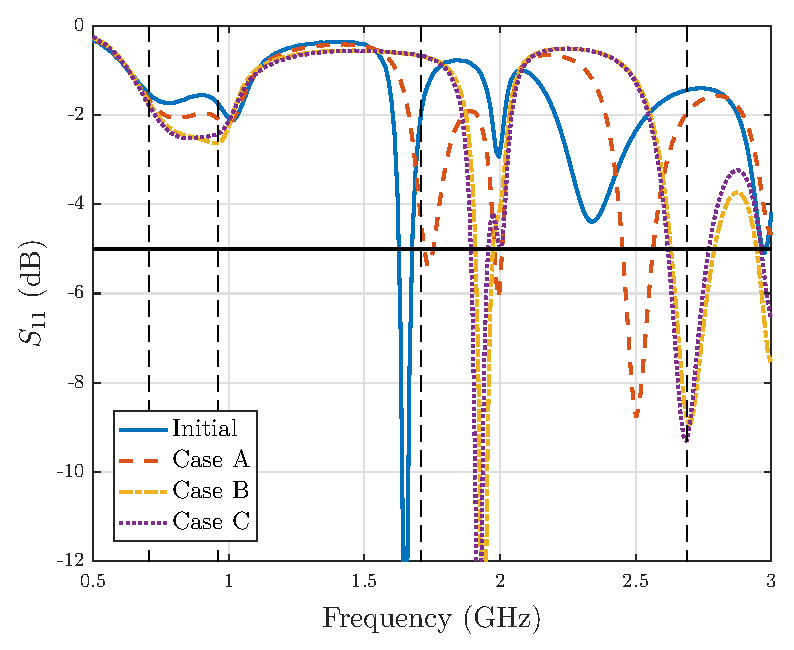
\includegraphics[width=0.5\textwidth]{img/concept2.eps}
    \caption{The best results from the three test cases.}
    \label{fig:concept2}
\end{figure}

Since the response of Case C in the low band was wide and below $-2\,\db$, a matching circuit was generated for it with Optenni. The program was set generate three element circuit for either only low band or both bands aiming for the defined $-5\,\db$ matching level. Figure \ref{fig:concept2_match} presents the results. The desired matching level is reached in neither of the two settings. When only the low band is matched, a decent level of $-4\,\db$ on average is obtained. Adding the requirement for the high band does not create much difference to the situation without any matching circuits. 
\begin{figure}[H]
    \centering
    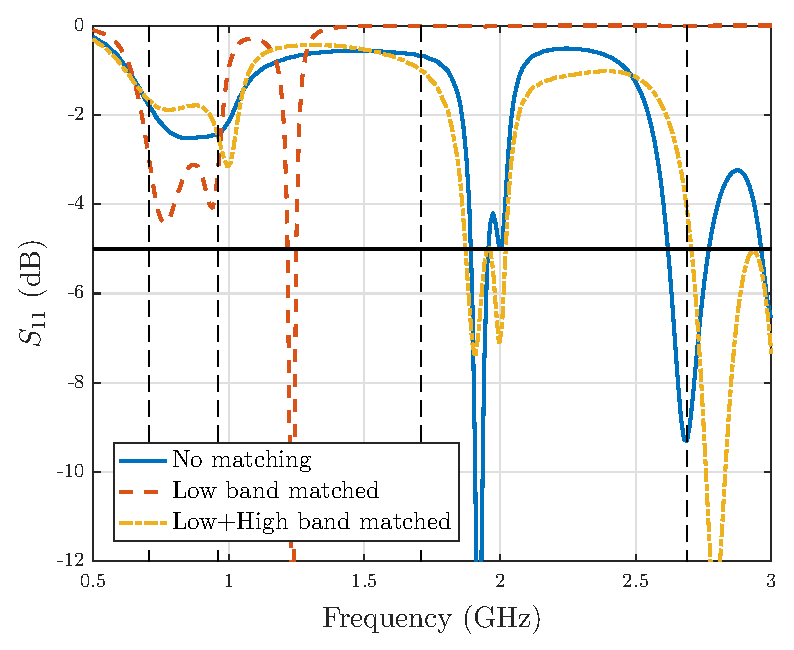
\includegraphics[width=0.5\textwidth]{img/concept2_match.eps}
    \caption{Matched antennas.}
    \label{fig:concept2_match}
\end{figure}

Since a suitable matching network could not be found for this structure, it means that the antennas should be modified more. One option would be to create two parallel matching circuits, one for low band and the other for high band. This however would increase the complexity of the system, which is undesired. Other possible solution could be modifying the antenna structures to be asymmetric, which would be the preferable choice of the two mentioned options.

Asymmetric structures were tested with four different cases. Case D has an offset in the location of the feed, which causes the top-parts of the L-shaped elements to have different lengths. In Case E, the antenna parts on the sides of the phone are of different length. For Case F the feed is transferred to the corner of an L-shaped element and in Case G, feed is offsetted from that location.

Again, only the best structures are presented of each case. Table \ref{tab:concept3} shows the changes in dimensions required in Cases D and E. In the best scenario of Case D the amount of offset was $3.5\,\milli\meter$ to the left and in Case G $5\,\milli\meter$ to the right. 
\begin{table}[H]
    \centering
    \caption{Changed dimensions to create asymmetry. All values are in millimeters.}
    \label{tab:concept3}
    \begin{tabular}{|c|c|c|}
        \hline
        \textbf{Dimension} & \textbf{Case D} & \textbf{Case E}\\
        \hline
        $l_1$ & 26 & 20 \\
        \hline
        $l_2$ & 33 & 33\\
        \hline
        $l_3$ & 40 & 40\\
        \hline
        $l_4$ & 26 & 30\\
        \hline
    \end{tabular}
\end{table}

Figure \ref{fig:concept_offsets} illustrates the structural changes of Cases D-G. The feed offset introduced in Case D is seen in Figure \ref{fig:concept3_u_offset}. The red dashed line shows the original location of the feed, in the middle of the side frame. Also the changes in the lengths of the L-elements (Case E) can be seen. Figure \ref{fig:concept_l_feed} shows the feeding structure of Case G, and the red dashed area points out the feed position of Case F.

\begin{figure}[H]
    \centering
    \begin{subfigure}[b]{0.49\textwidth}
        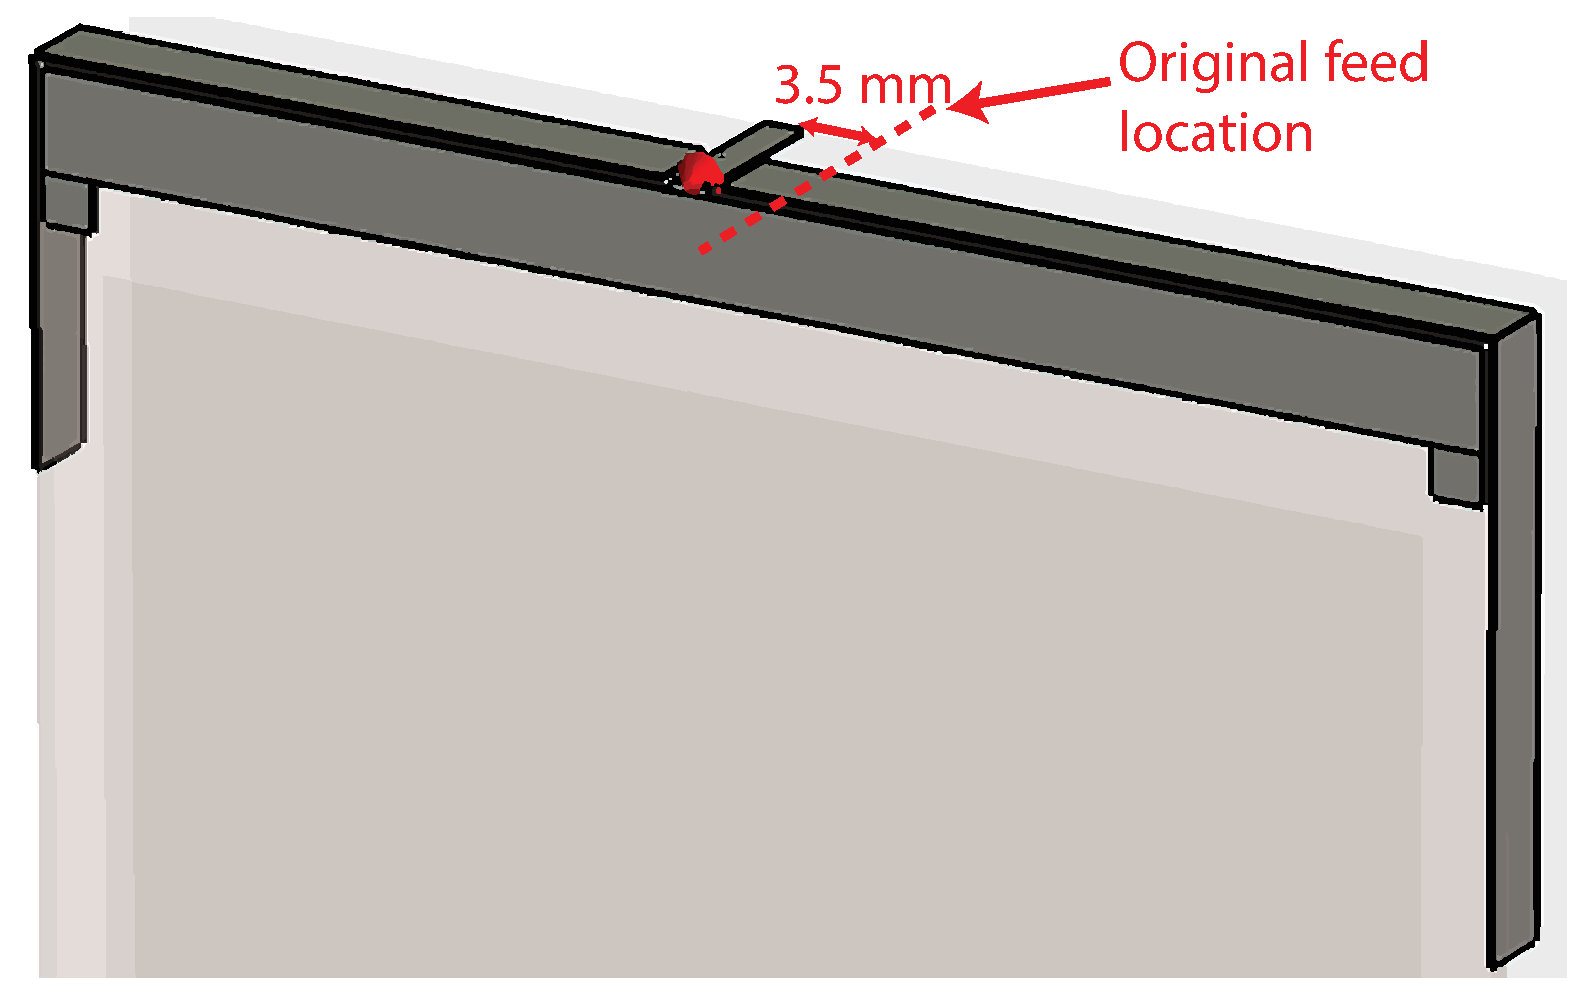
\includegraphics[width=\textwidth]{img/concept3_u_offset.eps}
        \caption{Feed offset in the U-shaped element.}
        \label{fig:concept3_u_offset}
    \end{subfigure}
    \begin{subfigure}[b]{0.49\textwidth}
        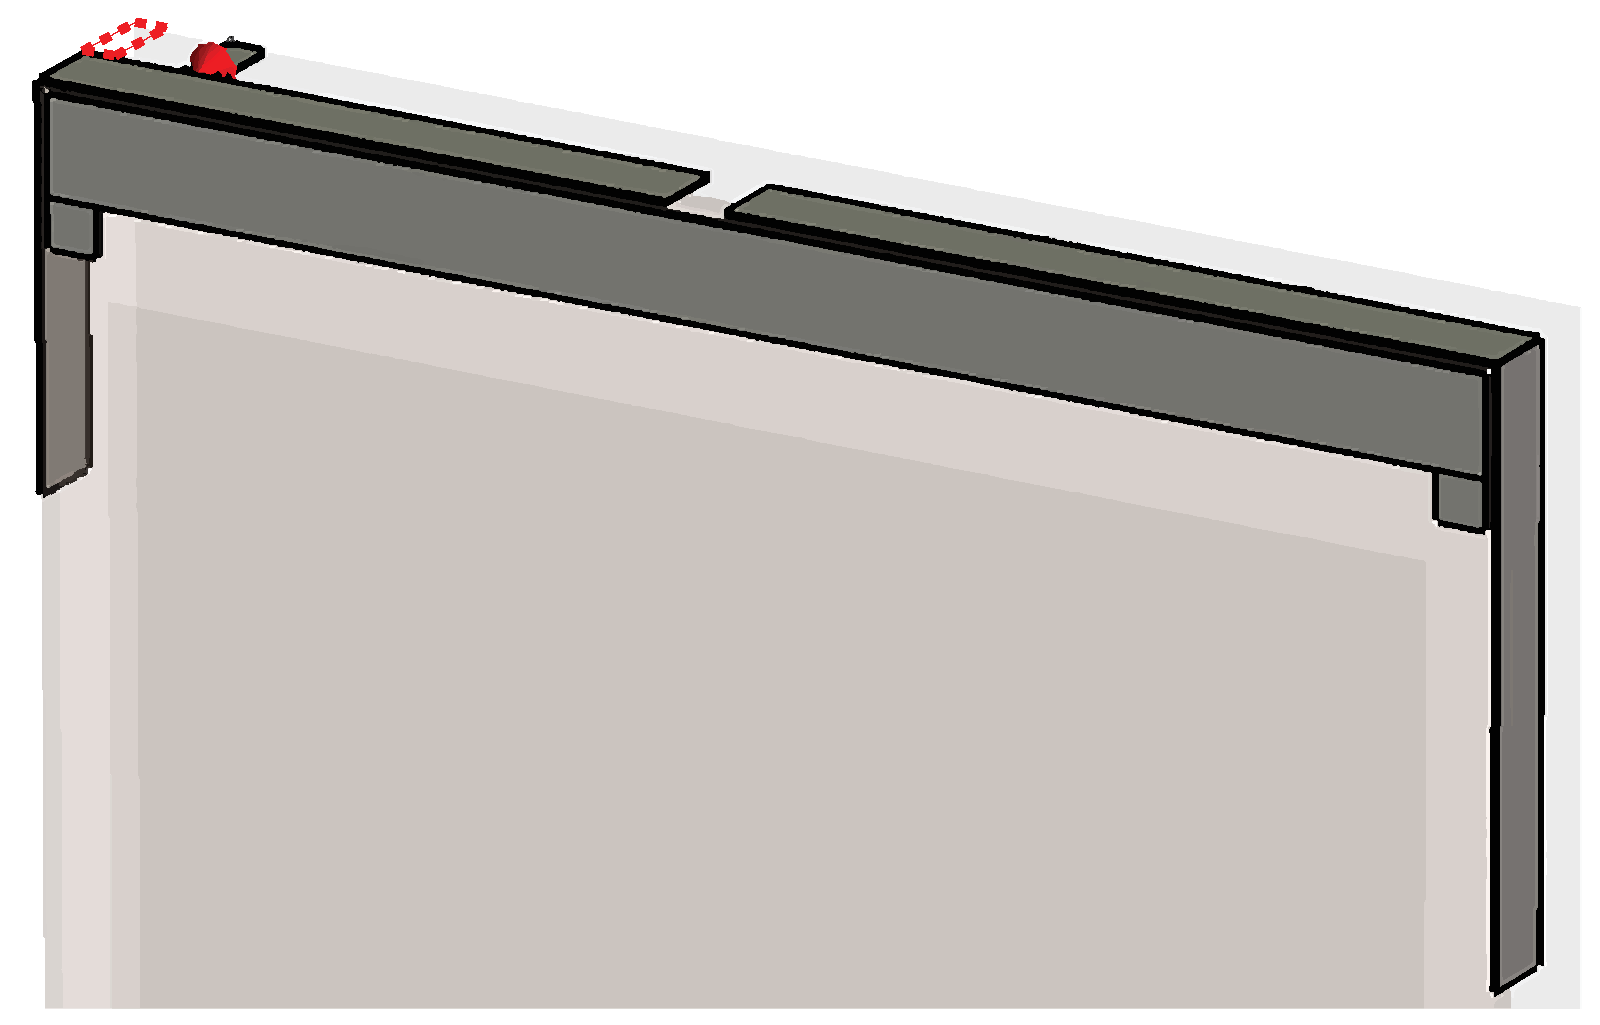
\includegraphics[width=\textwidth]{img/concept_l_feed.eps}
        \caption{Feed in the L-shaped element.}
        \label{fig:concept_l_feed}
    \end{subfigure}
    \caption{Changes in antenna structure in Cases D-G.}
    \label{fig:concept_offsets}
\end{figure}

Similarly as the cases with symmetric structures, the performance of the antenna system improved as the test cases proceeded, like Figure \ref{fig:concept3} represents. Matching in the low band is still wide and levels have increased. Besides that, also upper band is showing major enhancements, especially in Cases F and G. Matching levels are fair at the whole band. The only drawback is that the response in the high band resonates a lot, which might be a problem when generating matching circuits.
\begin{figure}[H]
    \centering
    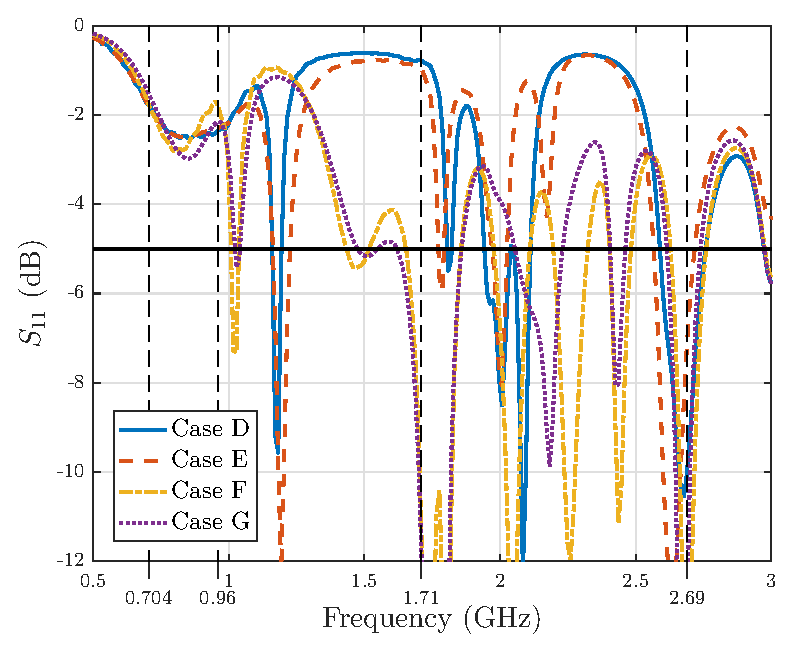
\includegraphics[width=0.5\textwidth]{img/concept3.eps}
    \caption{The best results from different asymmetric structures.}
    \label{fig:concept3}
\end{figure}

A matching network was generated also for the antenna of Case G. Optenni was set to construct matching circuits for either low band, high band, or both bands with target level of $-5\,\db$. Each topology had three components. Responses can be seen from Figure \ref{fig:concept3_match}. Surprisingly, responses are more or less identical, even with the one without matching circuits. In the low band a little more bandwidth is obtained when the antenna is matched, however, the matching level is still much worse than the target. In the high band, all topologies provide better matching but the target level is not completely reached. One curious observation is that Optenni resulted the same topology for matching only low band or both bands. It can be concluded that the environment is very challenging for designing low band antennas, and moreover, matching them.
\begin{figure}[H]
    \centering
    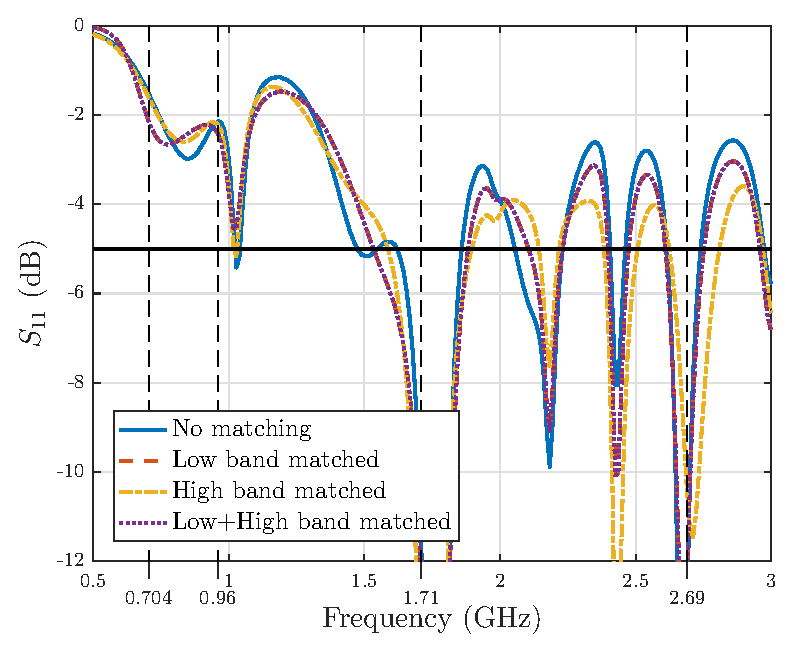
\includegraphics[width=0.5\textwidth]{img/concept3_match.eps}
    \caption{Different matching topologies.}
    \label{fig:concept3_match}
\end{figure}

At this point, it has been noticed, that the antenna concept requires some asymmetry in the structure, and also is quite precise of its dimensions. Next, the element above the display is modified. Case H changes the gap between the U-shaped element and the top of the phone from $0.5\,\milli\meter$ to $1\,\milli\meter$, which is seen as $w_2$ decreasing to $4.5\,\milli\meter$. The most radical modification is seen in Case I, where the barbs of the U-shaped element are removed, and only a straight metallic sheet is left (later referred as an I-shaped element). Figure \ref{fig:concept_i_shape} shows the updated structure.
\begin{figure}[H]
    \centering
    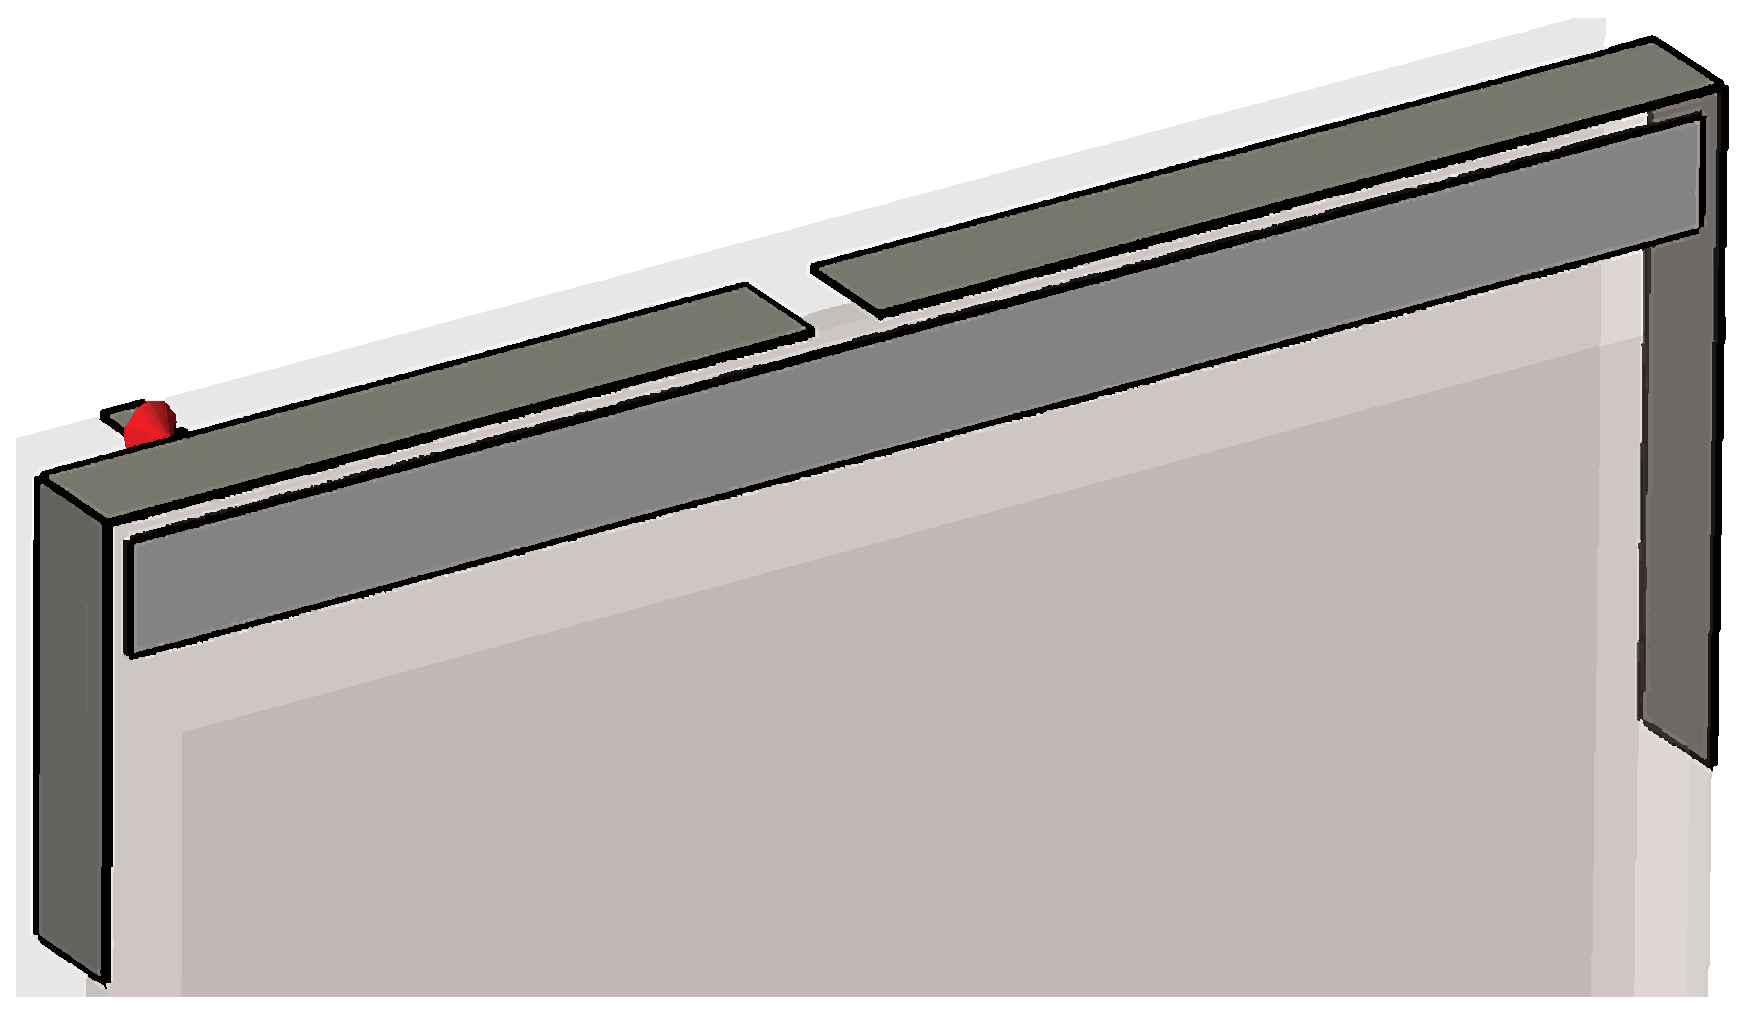
\includegraphics[width=0.5\textwidth]{img/concept_i_shape.eps}
    \caption{Antenna structure with the larger gap between elements from Case H and I-element from Case I.}
    \label{fig:concept_i_shape}
\end{figure}

Figure \ref{fig:concept4} shows the best results of Cases H and I, compared to Case G of the previous round of tests. It can be seen, that transforming the U-element to an I-element, was a good change. Even though the low band is a little off the required frequencies, achieved bandwidth is wider and smoother than in any test so far. Progress has also happened in the high band, where the response is not that resonating anymore. Instead, the overall shape is more even, and matching levels mainly better.
\begin{figure}[H]
    \centering
    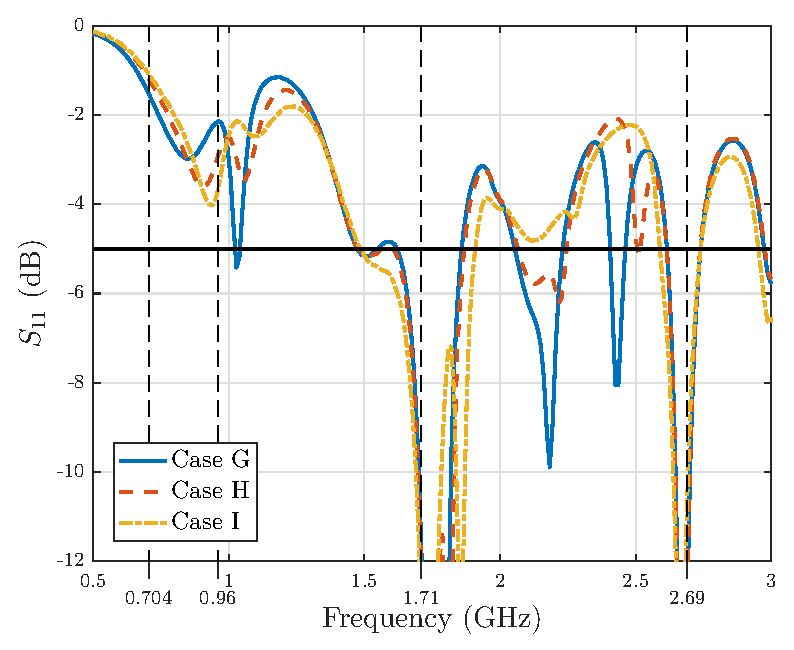
\includegraphics[width=0.5\textwidth]{img/concept4.eps}
    \caption{Simulation results from Cases H and I.}
    \label{fig:concept4}
\end{figure}

Last thing to test in the conceptualizing phase was using multiple feeds. So far, all structures in the pre-study and conceptualizing tests have had one feeding port. As this now studied structure consists of three separate but closely located elements, implementing multiple feeds would be a simple and straightforward process. This kind of system would have a few advantages. First, the mutual coupling effect might be stronger and enable larger achievable bandwidth. Second, matching the elements may be simpler since each feeding port can be assigned with its own set of frequencies. However, this will increase the complexity of the whole system.

Figure \ref{fig:concept_3feeds_struct} shows the modified structure for this test. Now the system has actually three antennas, named Element 1, 2, and 3, that are organized as marked in the figure.

The results are presented in Figure \ref{fig:concept_3feeds_res}. The matching of the low band nearly reaches the requirements as only a small set frequencies is uncovered. The performance of the high band is not as good, but still promising and the levels of Element 1 are mainly adequate keeping in mind that the antennas do not have any matching circuits yet.
\begin{figure}[H]
    \centering
    \begin{subfigure}[b]{0.49\textwidth}
        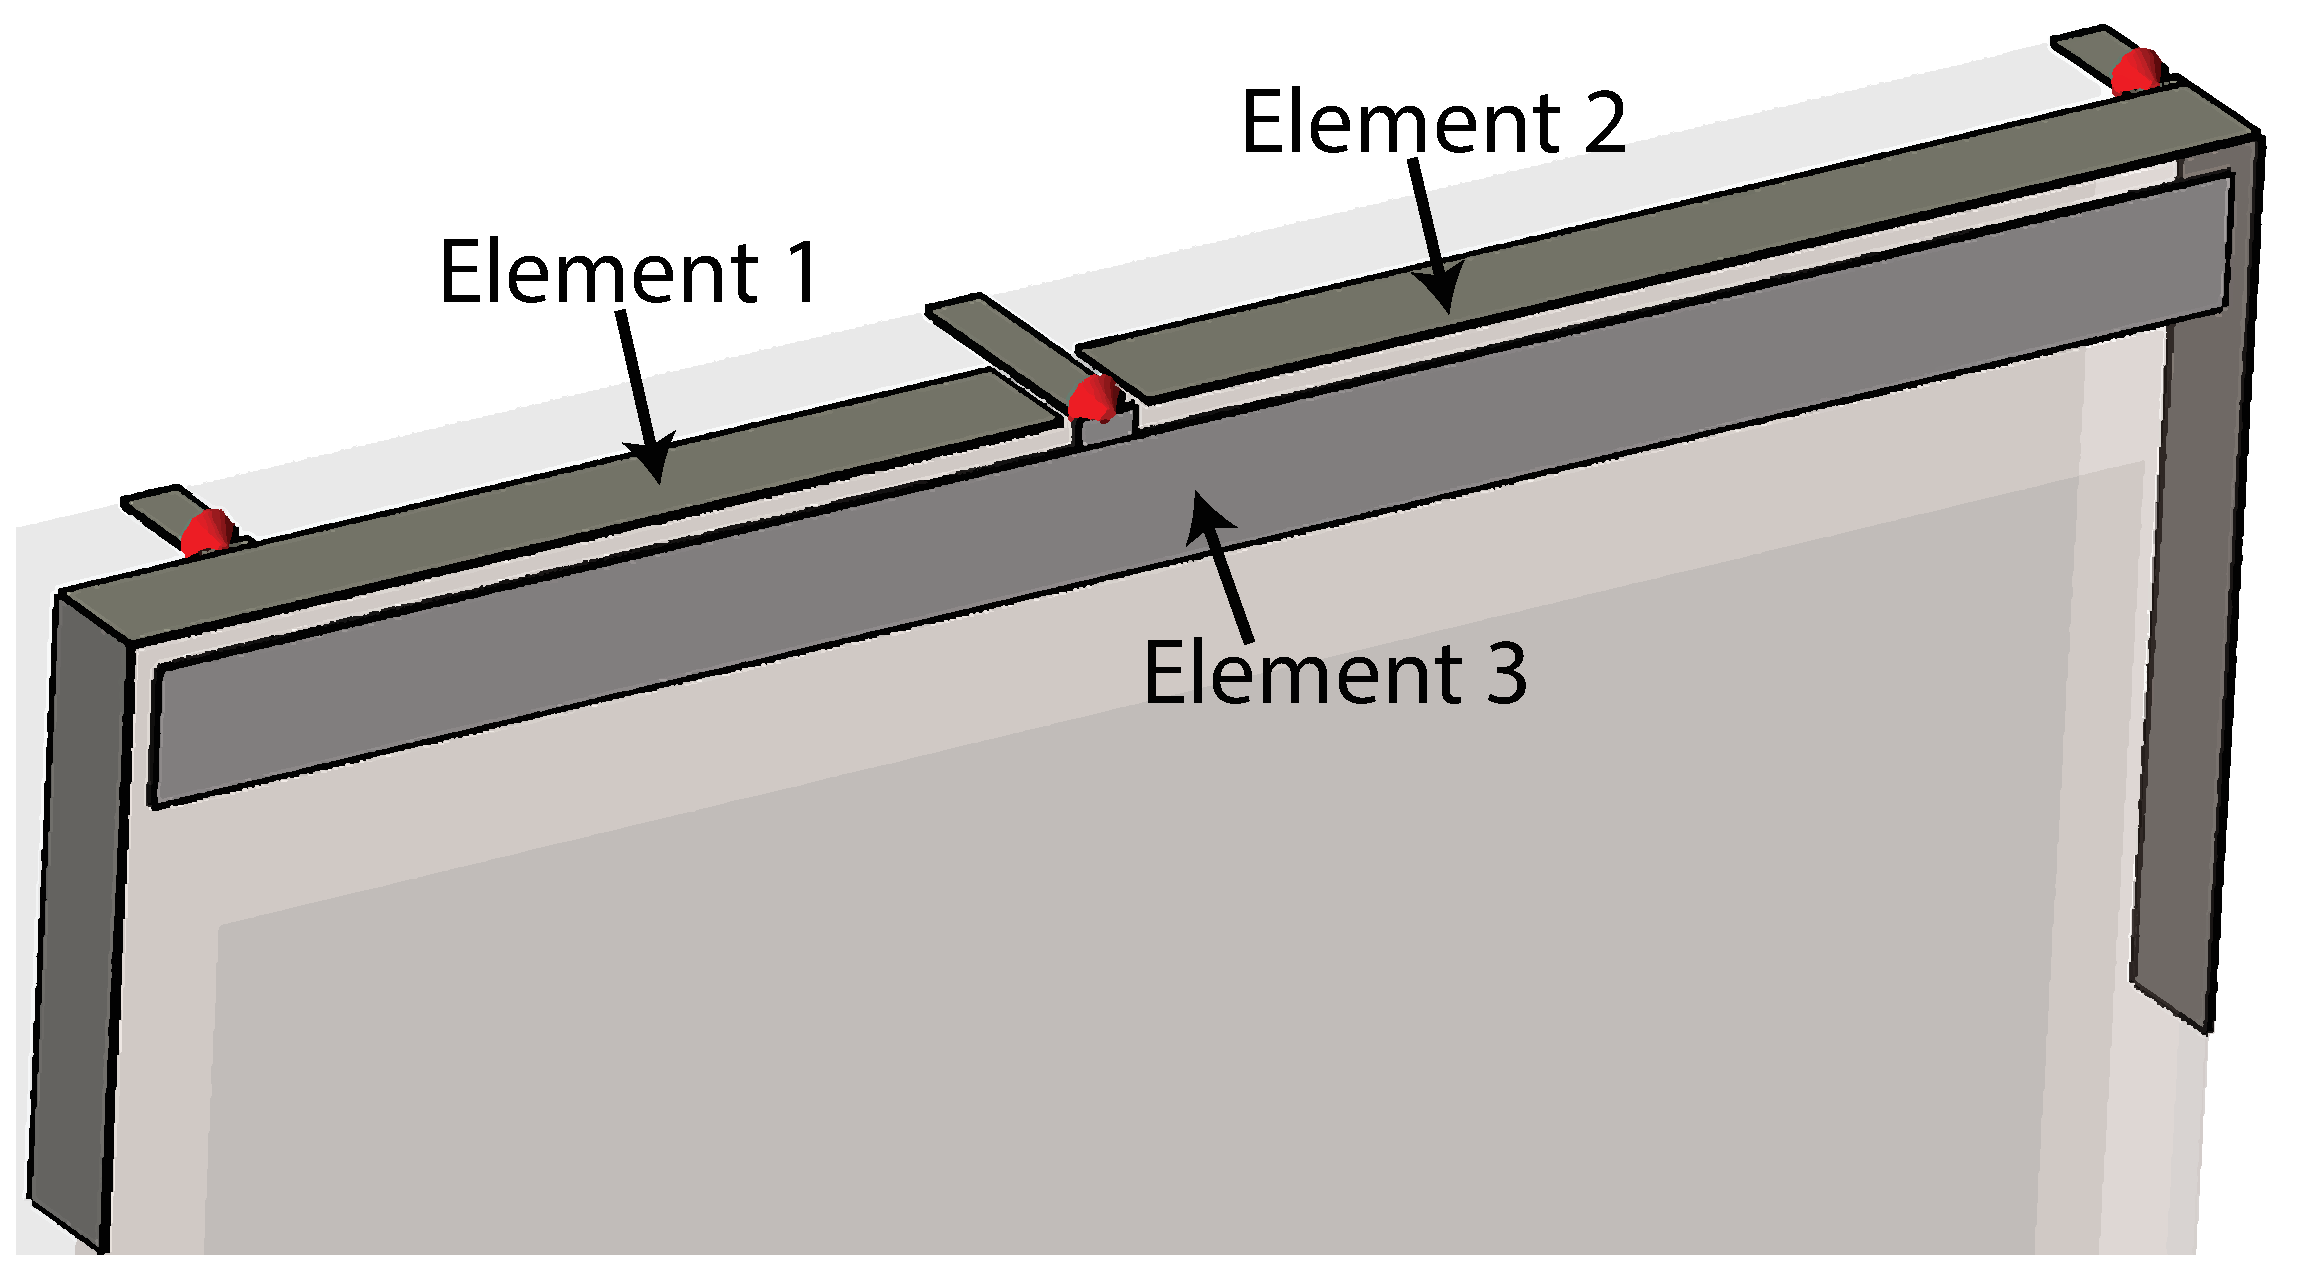
\includegraphics[width=\textwidth]{img/concept_3feed_struct.eps}
        \caption{Structure.}
        \label{fig:concept_3feeds_struct}
    \end{subfigure}
    \begin{subfigure}[b]{0.49\textwidth}
        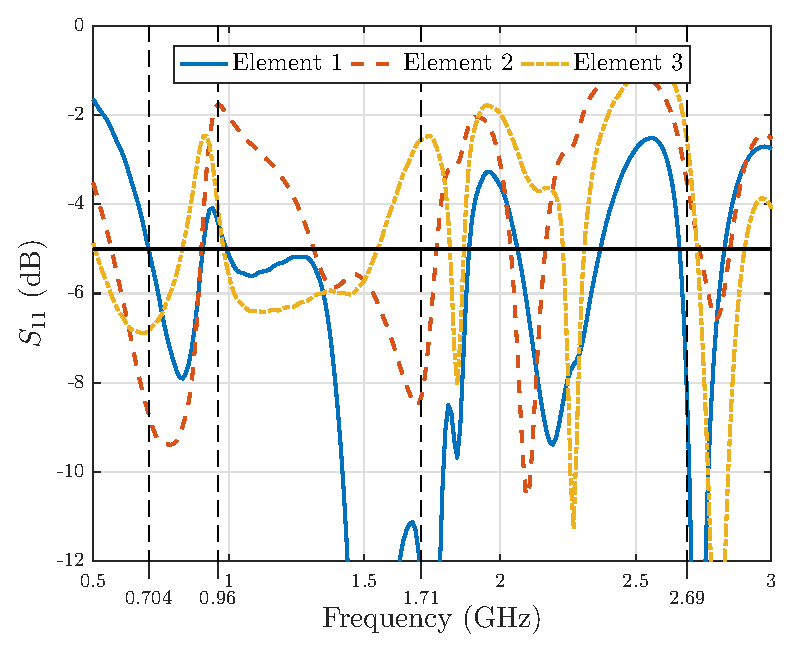
\includegraphics[width=\textwidth]{img/concept_3feeds.eps}
        \caption{Results.}
        \label{fig:concept_3feeds_res}
    \end{subfigure}
    \caption{Antenna simulation with three feeds.}
    \label{fig:concept_3feeds}
\end{figure}



\subsection{Simulations with realistic model}
\label{sec:sim_realistic}
For this project, it was specified to use mechanically very accurate 3D-model of a real smart phone to simulate the antennas. The model was, however, simplified a lot to keep simulation times reasonable and modifying the antennas easier. Still, in addition to the metal cover, side frame, and antennas themselves, this model had a lot of other details like battery, USB-port, front camera, touchscreen buttons, and supportive structures like plastic rim or metallic middle frame. Otherwise the model was shaped like a simple box, except the plastic frame that was imported straight from the 3D-model. Rounded corners would have complicated creating and placing antenna elements to the model. Also, the difference in results was thought to be minimal. 

The simplified model is presented in Figure \ref{fig:realistic_model1} highlighting all the required details except the battery, which is underneath the middle frame. Figure \ref{fig:realistic_model2} illustrates the dimensions of the antenna structure. The different parts are labeled equally to the conceptualizing phase to keep the two models comparable.
\begin{figure}[H]
    \centering
    \begin{subfigure}[b]{0.5\textwidth}
        \includegraphics[width=\textwidth]{img/realistic_model1.eps}
        \caption{Simplified model of a mobile phone.}
        \label{fig:realistic_model1}
    \end{subfigure}
    
    \begin{subfigure}[b]{0.5\textwidth}
        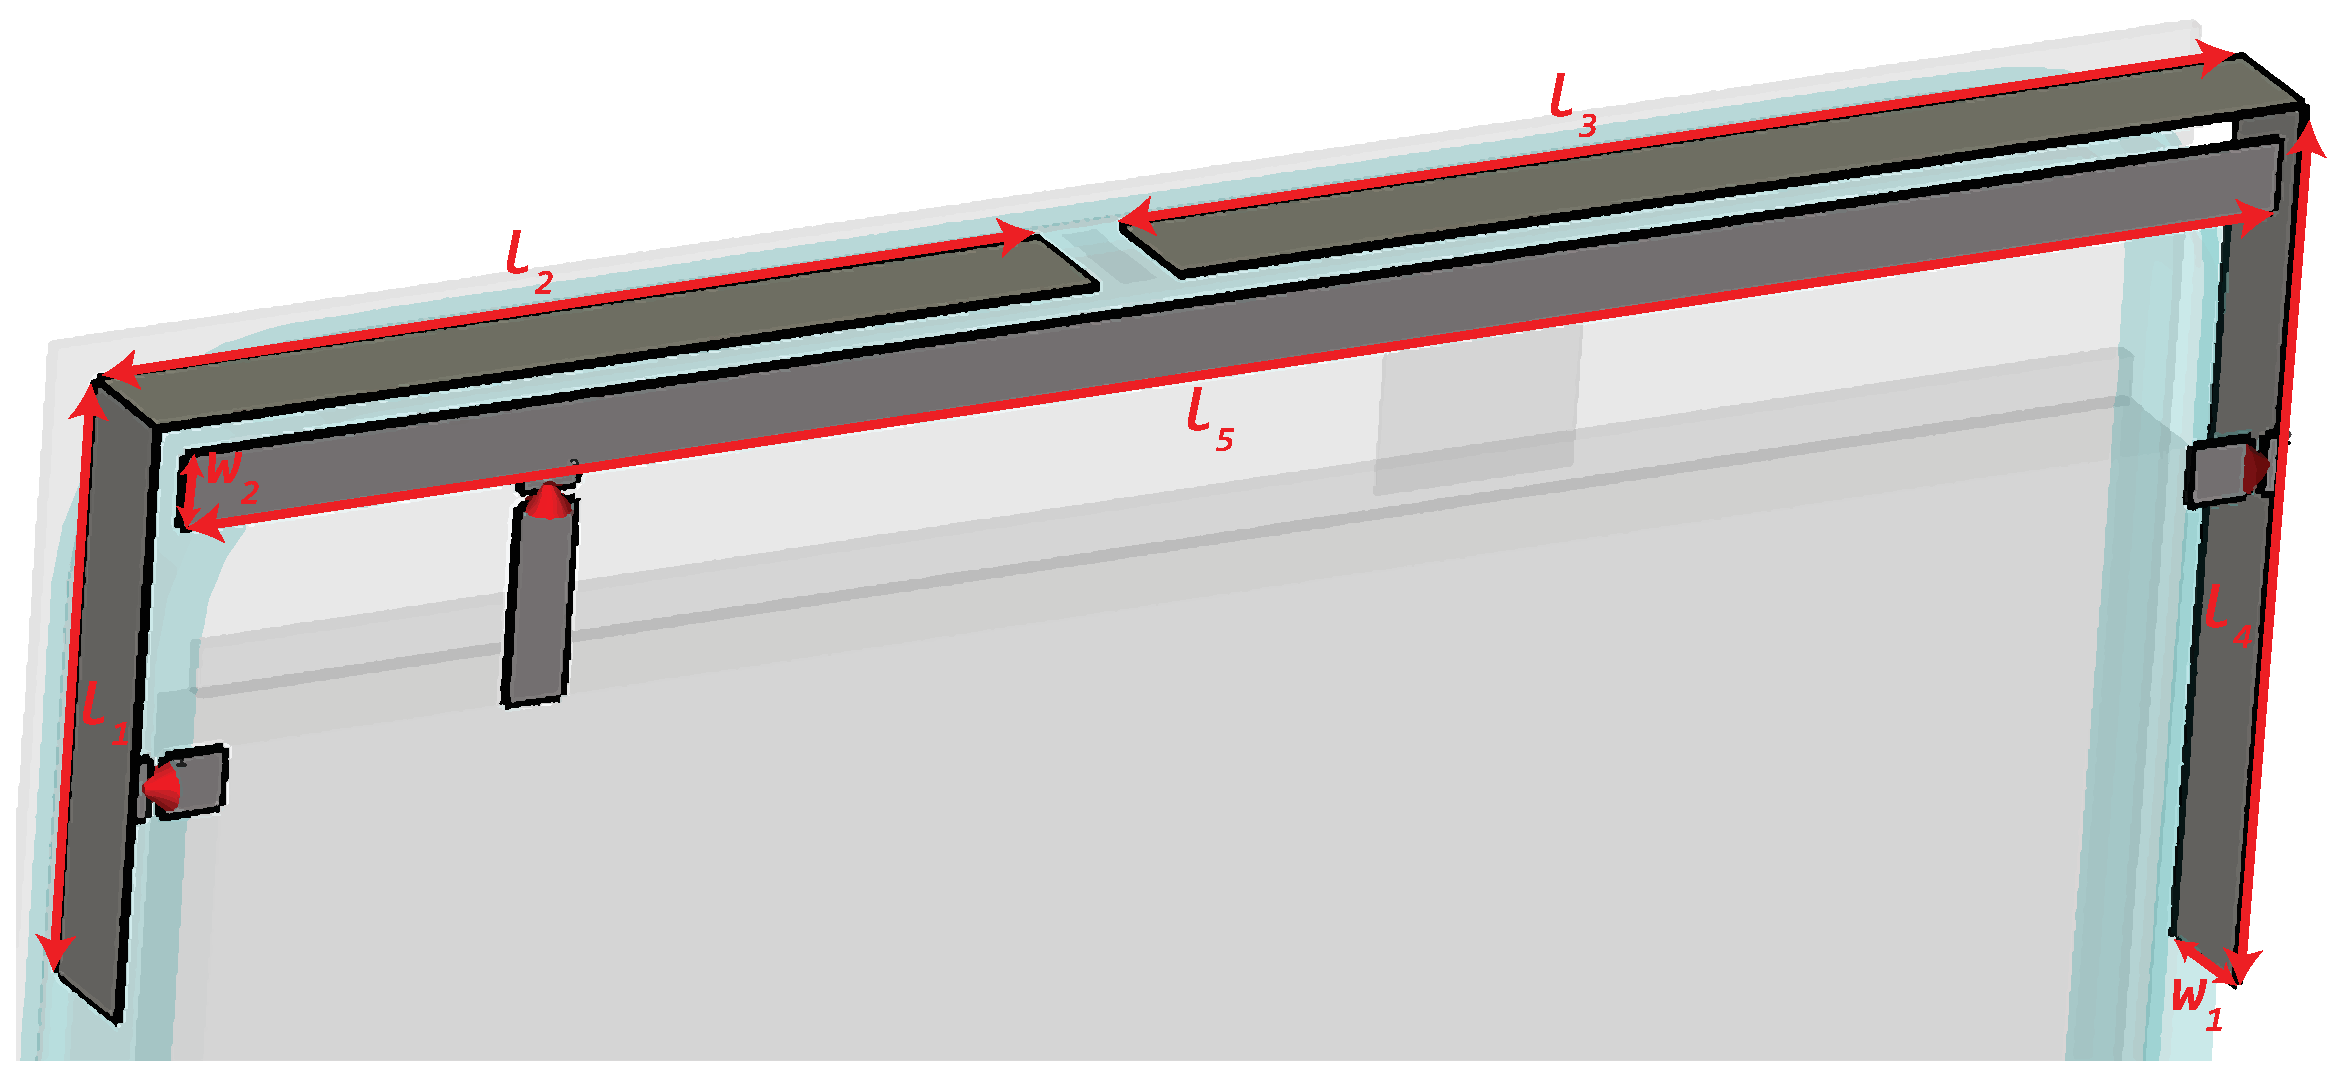
\includegraphics[width=\textwidth]{img/realistic_model2.eps}
        \caption{Structural dimensions of the main antenna.}
        \label{fig:realistic_model2}
    \end{subfigure}
    \caption{Illustrations of the realistic model and the antenna structure.}
    \label{fig:realistic_model}
\end{figure}

Simulations with this model were started by transferring the best structure from plain model simulations to the realistic model. Besides the amount of details in the new model, the only differences were the widths of the antennas ($w_1$ and $w_2$) and the feeding structure. The values of $w_1$ was pretty much determined by the actual 3D-model of a phone and $w_2$ had to be thinner since wider antenna would have blocked the front camera. Other dimensions stayed the same as the values of Case E listed in Table \ref{tab:concept3} earlier.

Antennas were fed from the middle frame. As previous tests had shown, the back cover should be used as a ground plane, and therefore the middle frame was connected with grounding pins to the back cover. This choice would be more suitable for a consumer product and a prototype could be built easier this way. 

As it can be seen from Figure \ref{fig:main_orig}, the more realistic environment has an effect on antennas. Comparing with Figure \ref{fig:concept_3feeds_res}, the matching levels for Elements 2 and 3 are lot better, though this is mainly due to strong mutual coupling. Increased amount of metallic structures in the model causes the currents to distribute differently, which is seen as a different response. Anyway, this proves the antenna concept to be usable for this project.
\begin{figure}[H]
    \centering
    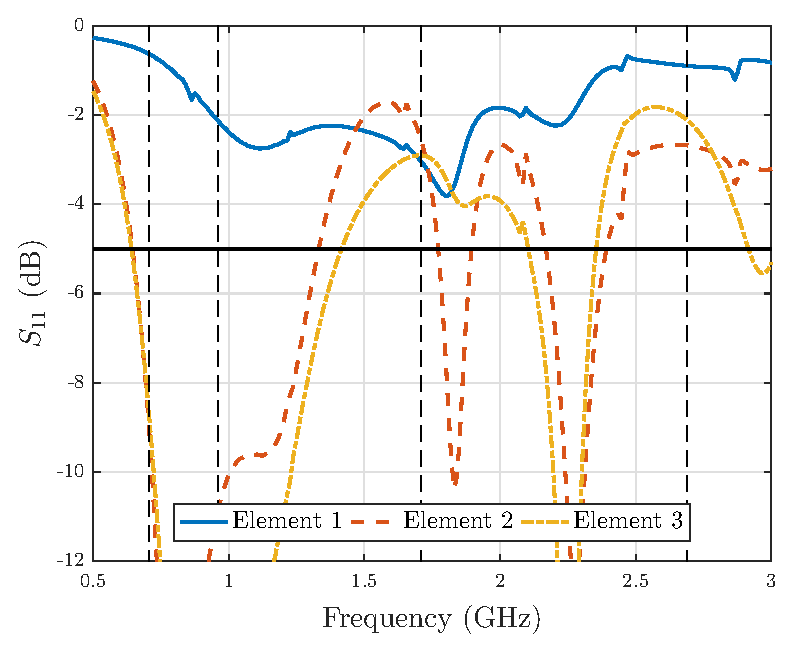
\includegraphics[width=0.5\textwidth]{img/main_orig.eps}
    \caption{Original matching levels of the concept antenna in realistic environment.}
    \label{fig:main_orig}
\end{figure}

The antenna structure was tested the same ways as with the plain model. As the structure was discovered to perform well in the plain model tests in both the low and the high band, it was believed that complete reconstruction would not be needed for the realistic model. Only dimensions of antenna elements and positions of the feeds were optimized. The final structure is shown in Figure \ref{fig:main_final} and the dimensions of each element are listed in Table \ref{tab:main_final}. As it can be seen from the figure, the L-shaped antennas are integrated into the metal rim on the side. The rim is not unbroken, and the gaps are $4.43\,\milli\meter$ on the sides and $2\,\milli\meter$ on the top. Clearance between the I-antenna and the L-antennas is $0.6\,\milli\meter$ at the end of the phone and $1.5\,\milli\meter$ in the sides.

More significant changes were made in the feeds. Besides adjusting their positions, them were after all moved to be connected to the back cover instead of the middle frame. Even though the middle frame was grounded from several locations, connecting the feeds to the back cover gave better bandwidth. However, this feeding structure is considerably more difficult to realize due to the limited space. The feeding pin is connected to the cover in the narrow area between the middle frame and the plastic rim, which does not leave much room for matching components or feeding cables in the real world.

\begin{figure}[H]
    \centering
    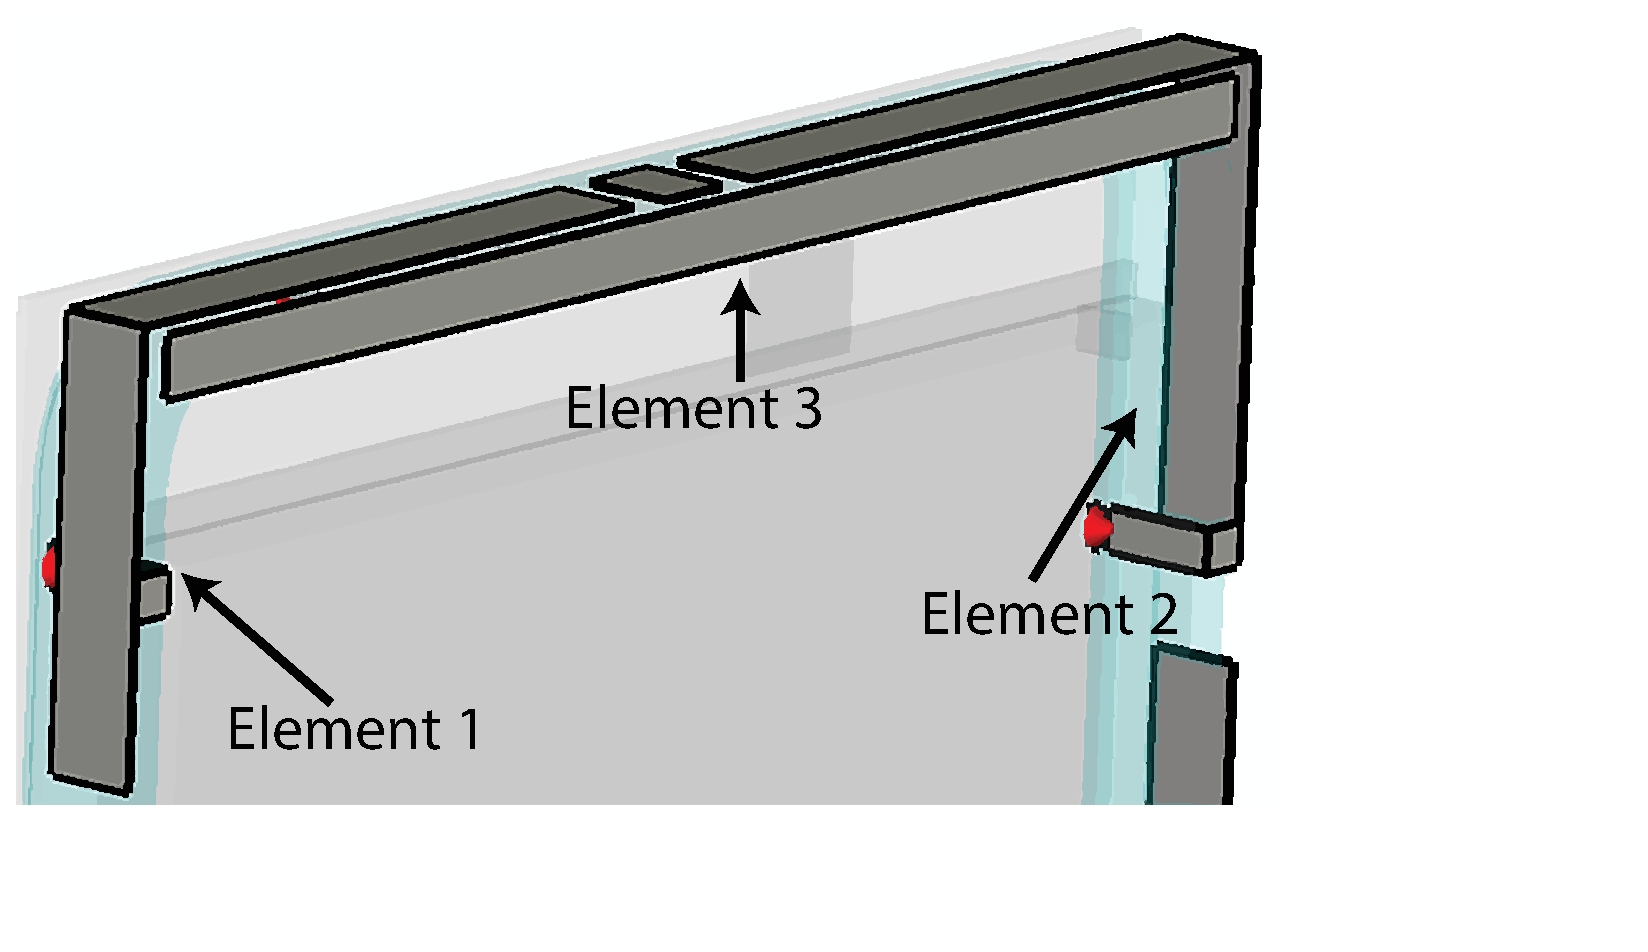
\includegraphics[width=0.5\textwidth]{img/main_final.eps}
    \caption{The final structure for the main antenna.}
    \label{fig:main_final}
\end{figure}
\begin{table}[H]
    \centering
    \caption{The dimensions of the final antenna structure.}
    \label{tab:main_final}
    \begin{tabular}{|c|c|}
        \hline
        \textbf{Dimension} & \textbf{Value [$\milli\meter$]}\\
        \hline
        $l_1$ & 20.76 \\
        \hline
        $l_2$ & 33\\
        \hline
        $l_3$ & 34.85 \\
        \hline
        $l_4$ & 23.23 \\
        \hline
        $l_5$ & 72.8 \\
        \hline
        $w_1$ & 4.35\\
        \hline
        $w_2$ & 2.9\\
        \hline
    \end{tabular}
\end{table}


At this point also matching networks gained more focus. It was found out already during the plain model simulations, that the desired matching level of $-5\,\db$ or efficiency of $30\,\%$ for the whole operating bands would not be reached without external matching circuits, and that finding a good matching network is not an easy task.

As mentioned earlier, the purpose of having three elements close to each other was to have strong coupling between them to achieve wider operational band. However, this coupling effect also complicated matching the elements. In many cases, the reflection coefficients of each element were very similar with at least one of the other elements. Figure \ref{fig:main_final_res} shows that effect with Elements 2 and 3. A huge band is obtained with substantial matching level by either of the elements. The mutual coupling between the antenna elements is shown in Figure \ref{fig:main_final_res_coup}. The figure presents the $S_{ij}$-parameters of the antenna system where indexes $i$ and $j$ refer to the respective antenna elements. The mutual coupling is strong between elements 2 and 3 in the low band, and this caused the elements to behave the same way while adding matching circuits. In other words, even if the matching level was suitable, nothing radiated since all the power flowed to other ports. Due to this harmful effect the structure was modified throughout the simulations to have asymmetry between the elements and their behavior, but the differences were not significant, and therefore the problem had to be solved with good matching circuits.

\begin{figure}[H]
    \centering
    \begin{subfigure}[b]{0.49\textwidth}
        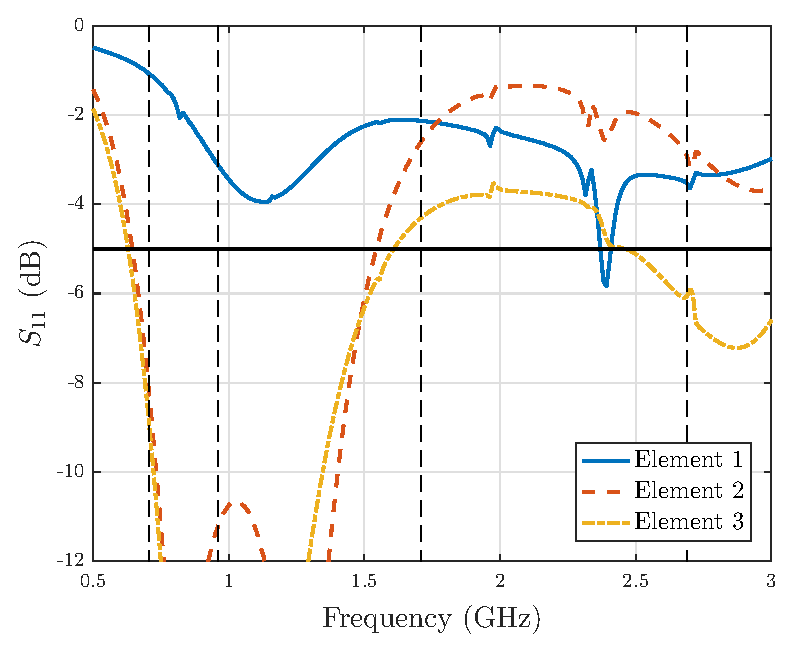
\includegraphics[width=\textwidth]{img/main_final_res.eps}
        \caption{Matching of each element.}
        \label{fig:main_final_res}
    \end{subfigure}
    \begin{subfigure}[b]{0.49\textwidth}
        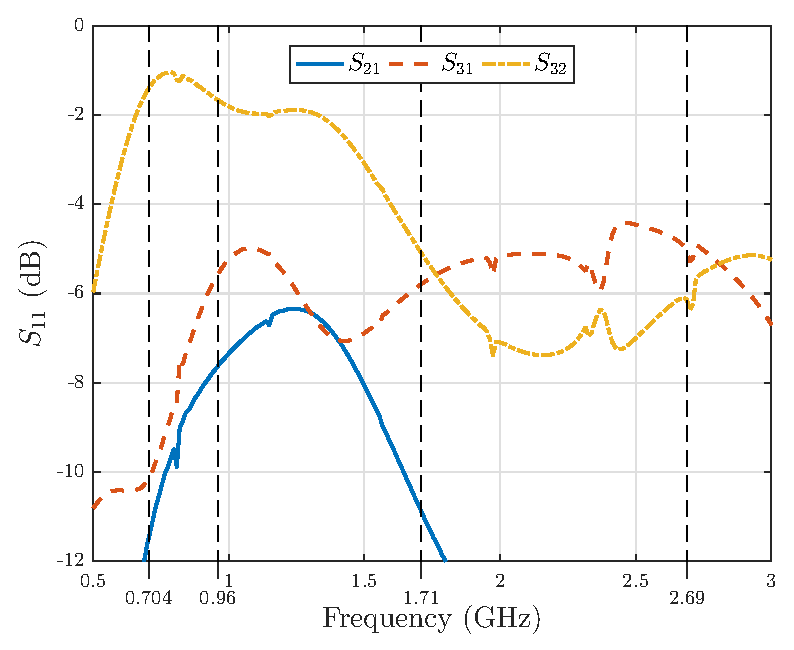
\includegraphics[width=\textwidth]{img/main_final_res_coup.eps}
        \caption{Mutual coupling.}
        \label{fig:main_final_res_coup}
    \end{subfigure}
    \caption{Performance of the final antenna before adding matching circuits.}
    \label{fig:main_res}
\end{figure}

For matching the antennas, the method was to mismatch other elements from the operational band to reduce negative coupling, and then match the radiating element. This was done with the help of antenna's impedance plots on the Smith chart. Location on the chart shows whether a capacitance or an inductance should be added to the circuit. With the help of Optenni Lab many different topologies and goals for matching could be tested quickly. The actual design and optimization of matching networks was done in NI AWR Design Environment.

Even though a goal for matching level had been defined for this thesis, efficiency was thought to be more important factor. Even if antennas were nearly perfectly matched, they might be very inefficient and thus, would not radiate. So, it was more critical to fulfill the goal for efficiency, even if it meant that matching level would not be sufficient. After many different tested matching circuits, two promising topologies were found. First option, presented in Figure \ref{fig:main_antenna_matching_circuits_opt1}, has 4 components for each antenna element, and the only radiating element is element 3. The other two are blocked and used only to increase bandwidth through coupling. The second possible design is shown in Figure \ref{fig:main_antenna_matching_circuits_opt2}. This topology oppositely blocks element 3, and radiates with element 2 in the low band and 1 in the high band. From now on, matching circuits of Figures \ref{fig:main_antenna_matching_circuits_opt1} and \ref{fig:main_antenna_matching_circuits_opt2} are referred as topologies 1 and 2, respectively.

\begin{figure}[H]
    \centering
    \begin{subfigure}[b]{0.4\textwidth}
        \begin{circuitikz}
            \draw 
                (0,0) to[short, o-] (1,0)
                (1,0) to[L, l^=$1\,\nano\henry$] (1,-2)
                (1,0) to[L, l^=$10.3\,\nano\henry$] (3,0)
                (3,0) to[C, l^=$1.8\,\pico\farad$] (3,-2)
                (3,0) to[L, l^=$20\,\nano\henry$] (5,0)
                (1,-2) node[ground]{}
                (3,-2) node[ground]{}
                (5,0) to[short] (5.5,0.5)
                (5,0) to[short] (5.5,-0.5);
        \end{circuitikz}
        \caption{Element 1.}
        \label{fig:main_match_11}
    \end{subfigure}
    \begin{subfigure}[b]{0.4\textwidth}
        \begin{circuitikz}
            \draw 
                (0,0) to[short, o-] (1,0)
                (1,0) to[C, l_=$10\,\pico\farad$] (1,-2)
                (1,0) to[L, l^=$6.6\,\nano\henry$] (3,0)
                (3,0) to[C, l^=$1\,\pico\farad$] (3,-2)
                (3,0) to[L, l^=$12.5\,\nano\henry$] (5,0)
                (1,-2) node[ground]{}
                (3,-2) node[ground]{}
                (5,0) to[short] (5.5,0.5)
                (5,0) to[short] (5.5,-0.5);
        \end{circuitikz}
        \caption{Element 2.}
        \label{fig:main_match_21}
    \end{subfigure}
    \begin{subfigure}[b]{0.4\textwidth}
        \begin{circuitikz}
            \draw 
                (1,0) to[C, o-, l^=$2.8\,\pico\farad$] (3,0)
                (3,0) to[L, l^=$10\,\nano\henry$] (3,-2)
                (3,0) to[C, l^=$1.9\,\pico\farad$] (5,0)
                (5,0) to[L, l^=$8.7\,\nano\henry$] (5,-2)
                (3,-2) node[ground]{}
                (5,0) to[short] (6,0)
                (5,-2) node[ground]{}
                (6,0) to[short] (6.5,0.5)
                (6,0) to[short] (6.5,-0.5);
        \end{circuitikz}
        \caption{Element 3.}
        \label{fig:main_match_31}
    \end{subfigure}
    \caption{Designed matching networks for the main antenna. Only element 3 radiates with this design.}
    \label{fig:main_antenna_matching_circuits_opt1}
\end{figure}


\begin{figure}[H]
    \centering
    \begin{subfigure}[b]{0.4\textwidth}
        \begin{circuitikz}
            \draw 
                (0,0) to[short, o-] (1,0)
                (1,0) to[C, l^=$1\,\pico\farad$] (1,-2)
                (1,0) to[C, l^=$2\,\pico\farad$] (3,0)
                (3,0) to[L, l^=$8.3\,\nano\henry$] (3,-2)
                (3,0) to[L, l^=$7.3\,\nano\henry$] (5,0)
                (1,-2) node[ground]{}
                (3,-2) node[ground]{}
                (5,0) to[short] (5.5,0.5)
                (5,0) to[short] (5.5,-0.5);
        \end{circuitikz}
        \caption{Element 1.}
        \label{fig:main_match_12}
    \end{subfigure}
    \begin{subfigure}[b]{0.4\textwidth}
        \begin{circuitikz}
            \draw 
                (1,0) to[L, o-, l^=$5.8\,\nano\henry$] (3,0)
                (3,0) to[C, l_=$7.4\,\pico\farad$] (3,-2)
                (4,0) to[L, l^=$8.7\,\nano\henry$] (4,-2)
                (4,0) to[L, l^=$12.1\,\nano\henry$] (6,0)
                (3,-2) node[ground]{}
                (4,-2) node[ground]{}
                (3,0) to[short] (4,0)
                (6,0) to[short] (6.5,0.5)
                (6,0) to[short] (6.5,-0.5);
        \end{circuitikz}
        \caption{Element 2.}
        \label{fig:main_match_22}
    \end{subfigure}
    \begin{subfigure}[b]{0.4\textwidth}
        \begin{circuitikz}
            \draw 
                (0,0) to[short, o-] (1,0)
                (1,0) to[C, l^=$1.7\,\pico\farad$] (1,-2)
                (1,0) to[C, l^=$9.9\,\pico\farad$] (3,0)
                (3,0) to[L, l^=$1\,\nano\henry$] (3,-2)
                (3,0) to[L, l^=$11.9\,\nano\henry$] (5,0)
                (1,-2) node[ground]{}
                (3,-2) node[ground]{}
                (5,0) to[short] (5.5,0.5)
                (5,0) to[short] (5.5,-0.5);
        \end{circuitikz}
        \caption{Element 3.}
        \label{fig:main_match_32}
    \end{subfigure}
    \caption{Designed matching networks for the main antenna. Element 3 is blocked while elements 1 and 2 radiate.}
    \label{fig:main_antenna_matching_circuits_opt2}
\end{figure}

Efficiencies for topologies 1 and 2 are presented in Figures \ref{fig:main_eff_top1} and \ref{fig:main_eff_top2}, respectively. It is clear, that topology 1 gives higher maximum efficiencies, but topology 2 covers the operational bands better. Topology 2 covers the low band totally, and only a small amount of the highest frequencies is below the required efficiency of $30\,\%$. The minimum of that part is ca. $27.5\,\%$ which can be considered close enough at this point. Other thing to support continuing with topology 2 is the shape of the curves, which are much smoother than with topology 1. Smoother curves provide more even efficiency throughout the band which leads to improved performance.

\begin{figure}[H]
    \centering
    \begin{subfigure}[b]{0.49\textwidth}
        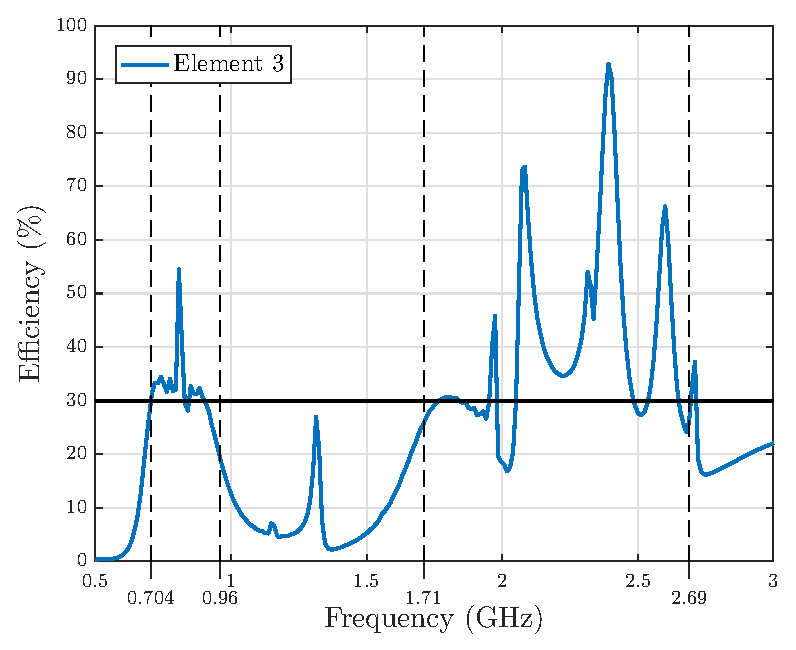
\includegraphics[width=\textwidth]{img/eff2_main.eps}
        \caption{Topology 1.}
        \label{fig:main_eff_top1}
    \end{subfigure}
    \begin{subfigure}[b]{0.49\textwidth}
        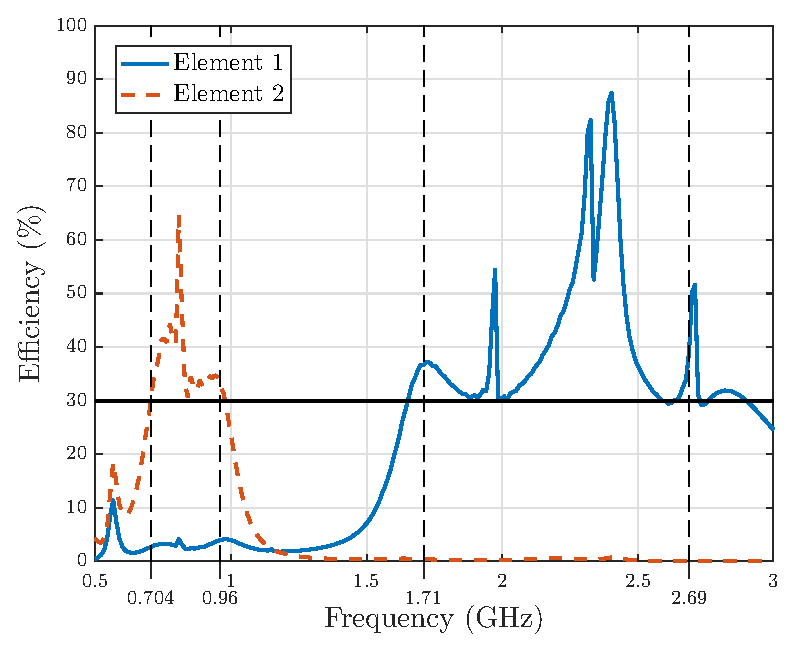
\includegraphics[width=\textwidth]{img/eff1_main.eps}
        \caption{Topology 2.}
        \label{fig:main_eff_top2}
    \end{subfigure}
    \caption{Efficiencies for main antenna with the two different matching networks.}
    \label{fig:main_eff}
\end{figure}

Now the main antenna has a decent performance in both the low and the high band covering them both almost completely.The matching levels with these circuits are presented in Figure \ref{fig:main_final_res_match}. It is seen that the levels are below the target level, but that can be considered to be acceptable while the efficiency requirement is fulfilled. The levels are anyhow fair, especially in the low band. Figure \ref{fig:main_final_res_match_coup} shows, that adding the matching circuits helped with the mutual coupling problem as the Element 3 is completely blocked. The antenna is able to radiate on a wide range of frequencies, as Figure \ref{fig:main_eff_top2} showed.  
\begin{figure}[H]
    \centering
    \begin{subfigure}[b]{0.49\textwidth}
        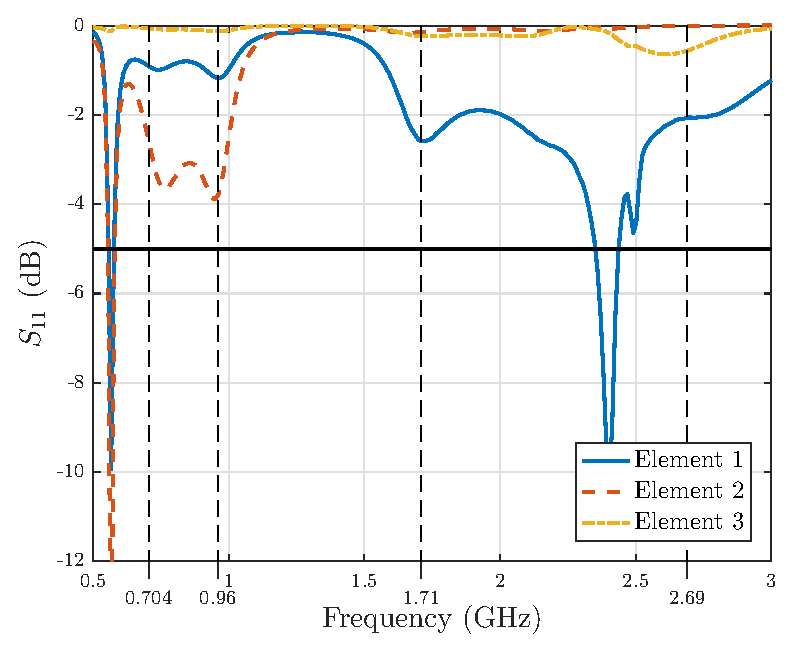
\includegraphics[width=\textwidth]{img/main_final_res_match.eps}
        \caption{Matching levels.}
        \label{fig:main_final_res_match}
    \end{subfigure}
    \begin{subfigure}[b]{0.49\textwidth}
        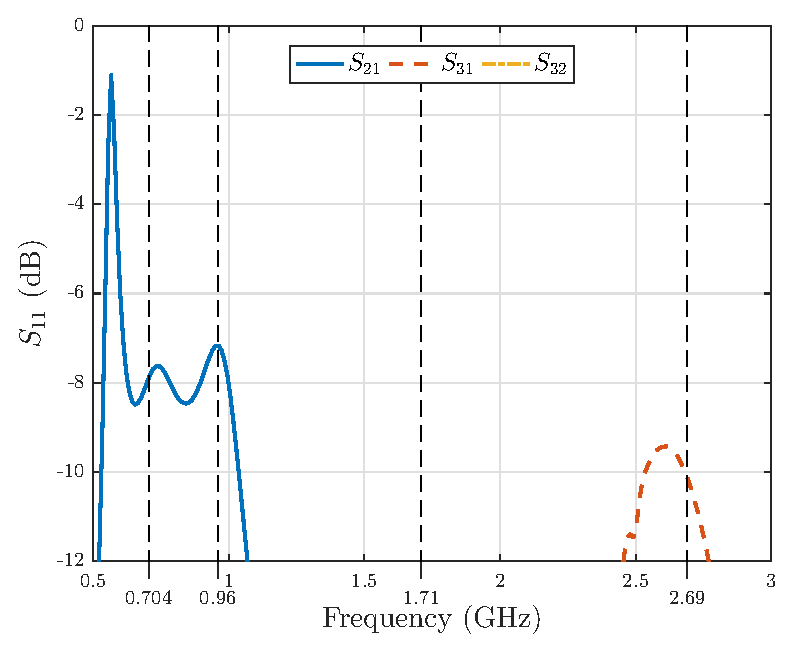
\includegraphics[width=\textwidth]{img/main_final_res_match_coup.eps}
        \caption{Mutual coupling.}
        \label{fig:main_final_res_match_coup}
    \end{subfigure}
    \caption{The performance of the matched main antenna.}
\end{figure}


\subsubsection{Diversity antenna}
\label{sec:diversity}
The phone was specified to have two cellular antennas, operating at the same set of frequencies in order to have MIMO capability. Since the diversity antenna should have similar performance as the main one, the same structure was used also for this second antenna. The main antenna was rotated $180\degree$ and placed to the other end of the phone. However, due to the USB-port and the touchpad buttons, exactly the same structure could not be used, but the basic concept was the same.

The dimensions of this antenna required only a little fine-tuning, as the main antenna was already an optimized structure. Figure \ref{fig:div_final} shows the final structure of the diversity antenna and the values of the labeled dimensions are listed in Table \ref{tab:div_final}. The most noticeable difference is the locations of the feeds. The differences between the distinct ends of the phone caused the optimal feed locations to be different. 
\begin{figure}[H]
    \centering
    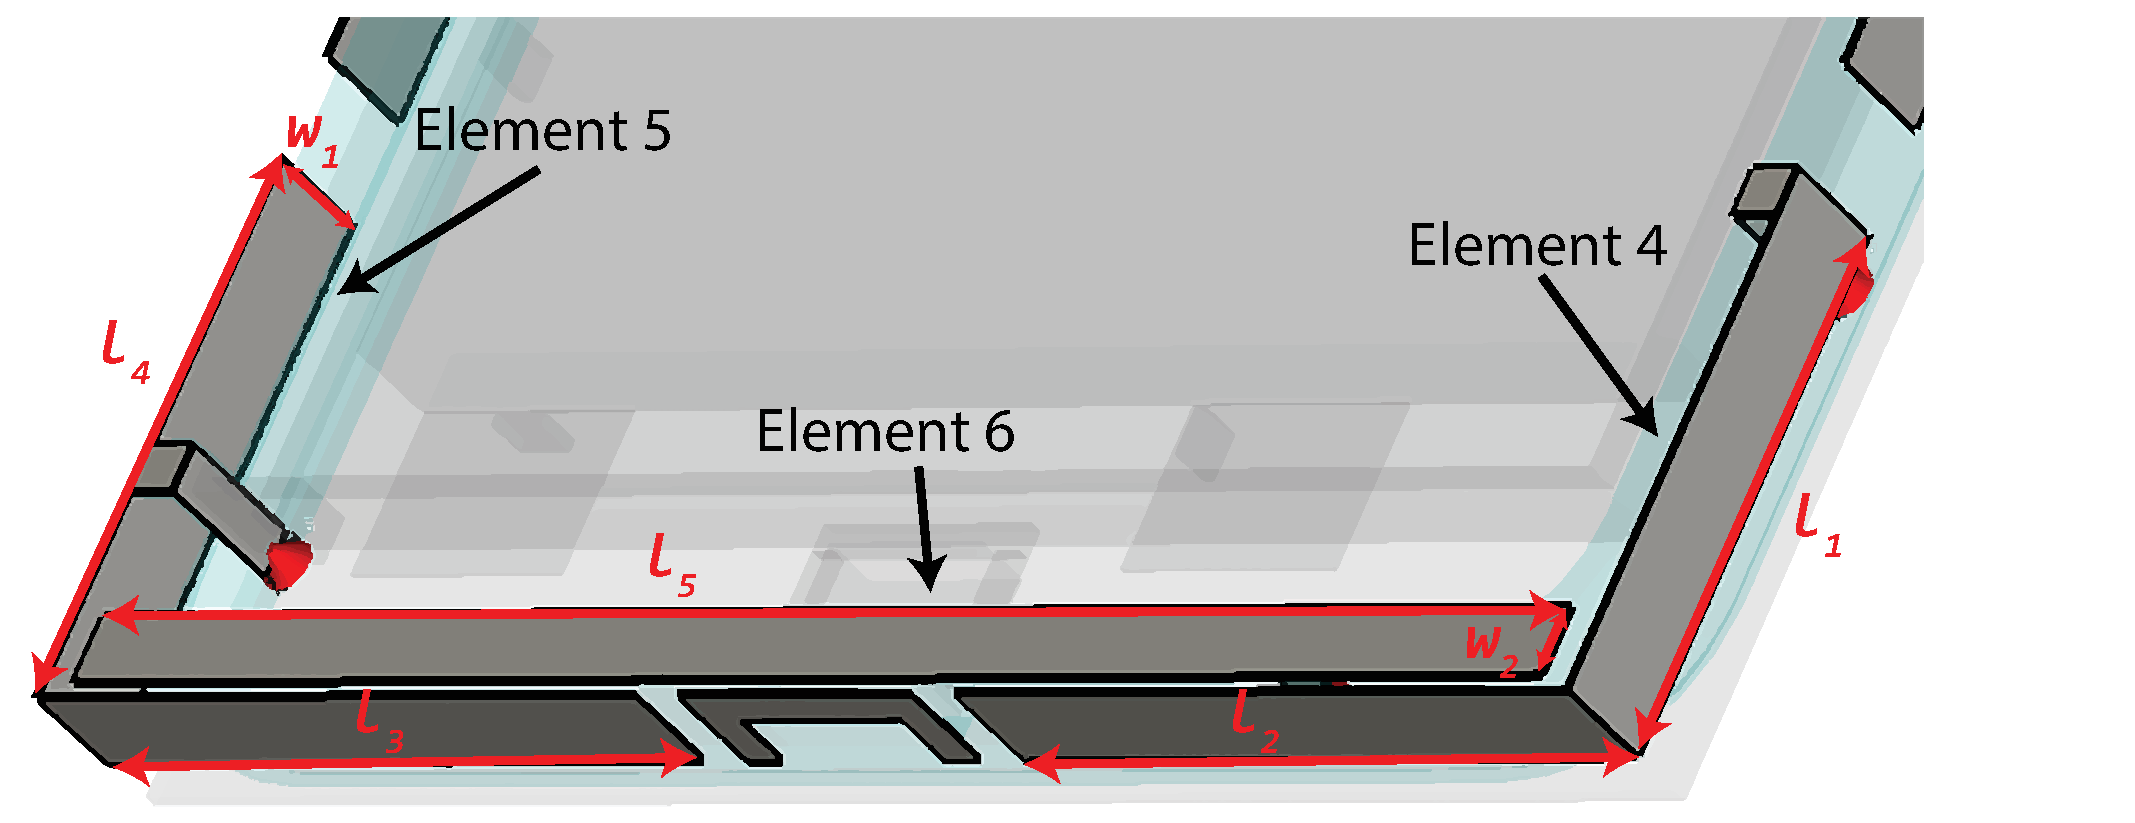
\includegraphics[width=0.5\textwidth]{img/diversity_final.eps}
    \caption{Structure of the diversity antenna.}
    \label{fig:div_final}
\end{figure}
\begin{table}[H]
    \centering
    \caption{The dimensions of the final diversity antenna.}
    \label{tab:div_final}
    \begin{tabular}{|c|c|}
        \hline
        \textbf{Dimension} & \textbf{Value [$\milli\meter$]}\\
        \hline
        $l_1$ & 22 \\
        \hline
        $l_2$ & 30\\
        \hline
        $l_3$ & 30 \\
        \hline
        $l_4$ & 23.23 \\
        \hline
        $l_5$ & 72.8 \\
        \hline
        $w_1$ & 4.35\\
        \hline
        $w_2$ & 2.9\\
        \hline
    \end{tabular}
\end{table}

Due to the similarity to the main antenna, the same matching circuits were applied, and only the component values optimized. Figure \ref{fig:div_match} shows the circuits with the component values for each element.
\begin{figure}[H]
    \centering
    \begin{subfigure}[b]{0.4\textwidth}
        \begin{circuitikz}
            \draw 
                (0,0) to[short, o-] (1,0)
                (1,0) to[C, l^=$1.1\,\pico\farad$] (1,-2)
                (1,0) to[C, l^=$2.1\,\pico\farad$] (3,0)
                (3,0) to[L, l^=$9.8\,\nano\henry$] (3,-2)
                (3,0) to[L, l^=$6.9\,\nano\henry$] (5,0)
                (1,-2) node[ground]{}
                (3,-2) node[ground]{}
                (5,0) to[short] (5.5,0.5)
                (5,0) to[short] (5.5,-0.5);
        \end{circuitikz}
        \caption{Element 4.}
        \label{fig:main_match_4}
    \end{subfigure}
    \begin{subfigure}[b]{0.4\textwidth}
        \begin{circuitikz}
            \draw 
                (1,0) to[L, o-, l^=$9.3\,\nano\henry$] (3,0)
                (3,0) to[C, l_=$5.8\,\pico\farad$] (3,-2)
                (4,0) to[L, l^=$18.6\,\nano\henry$] (4,-2)
                (4,0) to[L, l^=$17.9\,\nano\henry$] (6,0)
                (3,-2) node[ground]{}
                (4,-2) node[ground]{}
                (3,0) to[short] (4,0)
                (6,0) to[short] (6.5,0.5)
                (6,0) to[short] (6.5,-0.5);
        \end{circuitikz}
        \caption{Element 5.}
        \label{fig:main_match_5}
    \end{subfigure}
    \begin{subfigure}[b]{0.4\textwidth}
        \begin{circuitikz}
            \draw 
                (0,0) to[short, o-] (1,0)
                (1,0) to[C, l^=$1.3\,\pico\farad$] (1,-2)
                (1,0) to[C, l^=$8.3\,\pico\farad$] (3,0)
                (3,0) to[L, l^=$1\,\nano\henry$] (3,-2)
                (3,0) to[L, l^=$8.3\,\nano\henry$] (5,0)
                (1,-2) node[ground]{}
                (3,-2) node[ground]{}
                (5,0) to[short] (5.5,0.5)
                (5,0) to[short] (5.5,-0.5);
        \end{circuitikz}
        \caption{Element 6.}
        \label{fig:main_match_6}
    \end{subfigure}
    \caption{Matching circuits for the diversity antenna. Similarly to the main antenna, Element 6 is blocked while elements 4 and 5 radiate.}
    \label{fig:div_match}
\end{figure}

Figure \ref{fig:div_match_orig} shows that the same matching topologies are usable also for this antenna system. The target level is not reached at either of the bands, but on average the levels are decent. The most interesting discovery is that the main antenna is nearly not affected at all. The basic shape of the response is the same and only the sharp spikes have disappeared. The smoother curve might be result of simpler calculations done by CST. Now with the diversity antenna added, the antennas (ports) of the whole system are more symmetrical and balanced in the simulation model. This may yield a better convergence of energy in the system, and that way more accurate results. 
\begin{figure}[H]
    \centering
    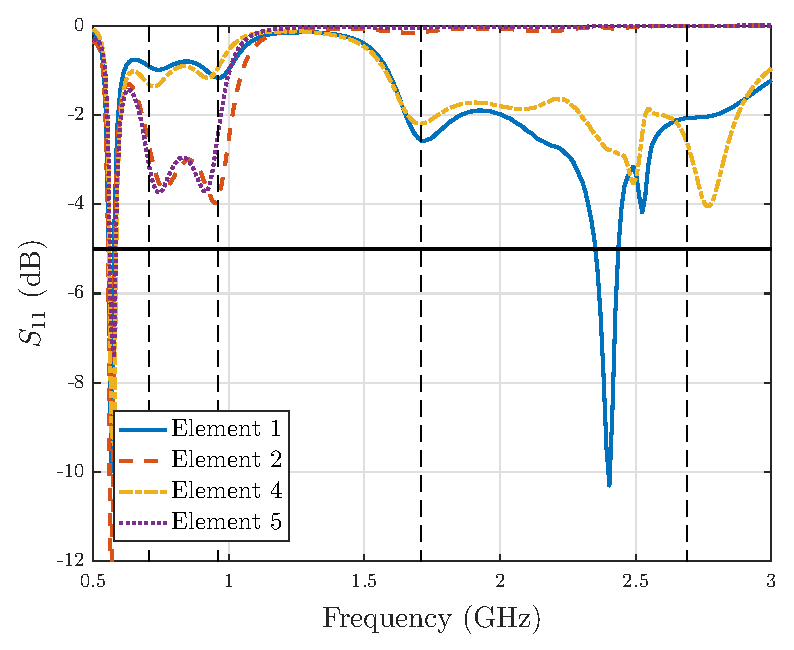
\includegraphics[width=0.5\textwidth]{img/diversity_match_orig.eps}
    \caption{Matching levels of the diversity antenna.}
    \label{fig:div_match_orig}
\end{figure}

Efficiency of the system behaves the same way, as Figure \ref{fig:div_eff_orig} presents. Both antennas more or less reach the target efficiency over the whole bands. As the antenna structures are now complete, the focus in the design of cellular antennas is passed to the matching circuits. Even though the existing topologies operate fine, they are far too complex. The number of components should be reduced for better understanding of the system, and also for easier realization of the system.
\begin{figure}[H]
    \centering
    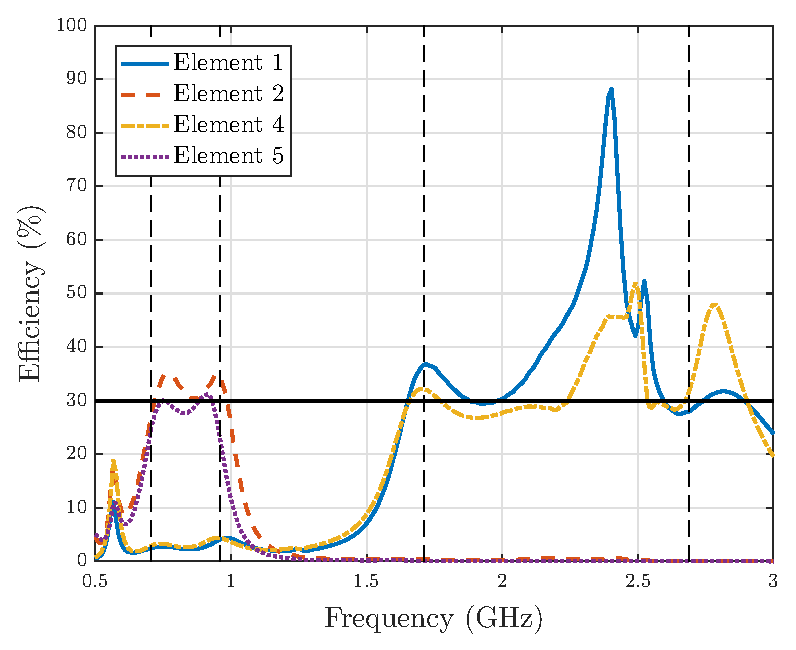
\includegraphics[width=0.5\textwidth]{img/diversity_eff_ideal_orig.eps}
    \caption{Efficiencies of the main and the diversity antennas.}
    \label{fig:div_eff_orig}
\end{figure}

\subsection{Improving the matching circuits}
\label{sec:matching_circuit}

Having four elements for each antenna element is a lot, especially when the system totally has six elements. Finding matching circuits with fewer components would be beneficial for a couple reasons. First, the total complexity of the system reduces, and that way the behavior of each component and element can be understood more thoroughly. Second, the system is more cost-effective and manufacturable when realized. 

By taking a new look at the designed matching circuits, it can be noticed that there are some unnecessary components. Large capacitors or small inductors behave electrically like short circuits, and likewise, small capacitors or large inductors as open circuits. Applying these electrical equivalences to the designed topologies, the circuits become significantly simpler, as Figure \ref{fig:simplified_circuits} shows. As the original component values were quite similar, the same modifications can be used in both cellular antennas. The most curious change is that Elements 3 and 6 are not fed anymore, but reactively loaded (Figure \ref{fig:simple_match_36}). As these elements were not radiating before and used only to enhance the performance of other elements, this new matching topology does not cause any problems. 

\begin{figure}[H]
    \centering
    \begin{subfigure}[b]{0.3\textwidth}
        \begin{circuitikz}
            \draw 
                (1,0) to[C, o-, l^=$C_1$] (3,0)
                (3,0) to[L, l^=$L_1$] (3,-2)
                (3,0) to[L, l^=$L_2$] (5,0)
                (3,-2) node[ground]{}
                (5,0) to[short] (5.5,0.5)
                (5,0) to[short] (5.5,-0.5);
        \end{circuitikz}
        \caption{Elements 1 and 4.}
        \label{fig:simple_match_14}
    \end{subfigure}
    \hspace{10pt}
    \begin{subfigure}[b]{0.3\textwidth}
        \begin{circuitikz}
            \draw 
                (1,0) to[L, o-, l^=$L_3$] (3,0)
                (3,0) to[C, l^=$C_2$] (3,-2)
                (3,0) to[L, l^=$L_4$] (5,0)
                (3,-2) node[ground]{}
                (5,0) to[short] (5.5,0.5)
                (5,0) to[short] (5.5,-0.5);
        \end{circuitikz}
        \caption{Elements 2 and 5.}
        \label{fig:simle_match_25}
    \end{subfigure}
    \hspace{10pt}
    \begin{subfigure}[b]{0.3\textwidth}
        \begin{circuitikz}
            \draw 
                (3,0) to[short] (3,-1)
                (3,0) to[L, l^=$L_5$] (5,0)
                (3,-1) node[ground]{}
                (5,0) to[short] (5.5,0.5)
                (5,0) to[short] (5.5,-0.5);
        \end{circuitikz}
        \caption{Elements 3 and 6.}
        \label{fig:simple_match_36}
    \end{subfigure}
    \caption{Simplified matching circuits.}
    \label{fig:simplified_circuits}
\end{figure}

After the simplification, the component values were reoptimized to better meet performance targets. The new component values are shown in Table \ref{tab:match} later on. Reducing the number of components affected the performance of the antennas. Actually the new topologies are slightly worse than the complex ones, which can be seen if \Cref{fig:div_eff_ideal,fig:div_ideal_match} are compared with \Cref{fig:div_match_orig,fig:div_eff_orig}. However, as the differences are so small and the requirement for efficiency is still nearly met, these new topologies can be considered better due to the reduced complexity.
\begin{figure}[H]
    \centering
    \begin{subfigure}[b]{0.49\textwidth}
        \includegraphics[width=\textwidth]{img/diversity_eff_ideal.eps}
        \caption{Efficiency.}
        \label{fig:div_eff_ideal}
    \end{subfigure}
    \begin{subfigure}[b]{0.49\textwidth}
        \includegraphics[width=\textwidth]{img/diversity_final_match.eps}
        \caption{Matching.}
        \label{fig:div_ideal_match}
    \end{subfigure}
    \caption{Antenna performances with simplified matching networks.}
    \label{fig:div_eff}
\end{figure}

So far all the matching components have been ideal capacitors or inductors. In order to have a better view of the actual performance of these antennas, the components replaced with realistic models of capacitors and inductors manufactured by Murata \cite{murata}. The used components were chosen from GQM1884 \cite{murata_c} and LQP03 \cite{murata_l} series. Component values are listed in Table \ref{tab:match}, together with the previously mentioned ideal components. Realistic component models have internal parasitic capacitances and inductances, and introduce losses to the circuit. These features affect the performance of an antenna, which is the reason for differences in component values between ideal and realistic models.
\begin{table}[H]
    \centering
    \caption{Component values for the matching circuits of Figure \ref{fig:simplified_circuits}.}
    \label{tab:match}
    \begin{tabular}{|c|c|c|c|c|}
        \hline
         & \multicolumn{2}{|c|}{Ideal components} & \multicolumn{2}{|c|}{Realistic components} \\
         \cline{2-5}
         Component & Main antenna & Diversity antenna & Main antenna & Diversity antenna\\
         \hline
         $C_1$ & $1.1\,\pico\farad$ & $1.4\,\pico\farad$ & $1.3\,\pico\farad$ & $1.5\,\pico\farad$\\
         \hline
         $C_2$ & $3.9\,\pico\farad$ & $3.7\,\pico\farad$ & $2\,\pico\farad$ & $2\,\pico\farad$\\
         \hline
         $L_1$ & $13\,\nano\henry$ & $10.5\,\nano\henry$ & $8.2\,\nano\henry$ & $6.8\,\nano\henry$\\
         \hline
         $L_2$ & $8.2\,\nano\henry$ & $4.1\,\nano\henry$ & $5.6\,\nano\henry$ & $1.8\,\nano\henry$\\
         \hline
         $L_3$ & $8.7\,\nano\henry$ & $11.7\,\nano\henry$ & $9.1\,\nano\henry$ & $10\,\nano\henry$\\
         \hline
         $L_4$ & $14.4\,\nano\henry$ & $19.9\,\nano\henry$ & $10\,\nano\henry$ & $13\,\nano\henry$\\
         \hline
         $L_5$ & $14\,\nano\henry$ & $9.2\,\nano\henry$ & $9.1\,\nano\henry$ & $6.8\,\nano\henry$\\
         \hline
    \end{tabular}
\end{table}

Changing from ideal components to realistic ones has a major effect on the performance of the antennas. Due losses of the lumped elements the antennas' performance improved significantly. As can be seen from the plots of Figure \ref{fig:div_real}, both antennas are operating wideband on good levels, fulfilling the requirements for efficiency. On average efficiencies are around $40\,\%$ on low band and around $50\,\%$ on high band. Moreover, the matching levels on the whole bands are on average below $-3\,\db$, which is clearly better than any designed antenna in this project has reached so far.

\begin{figure}[H]
    \centering
    \begin{subfigure}[b]{0.49\textwidth}
        \includegraphics[width=\textwidth]{img/diversity_final_real_match.eps}
        \caption{Matching levels.}
        \label{fig:div_match_real}
    \end{subfigure}
    \begin{subfigure}[b]{0.49\textwidth}
        \includegraphics[width=\textwidth]{img/diversity_eff_real.eps}
        \caption{Efficiencies.}
        \label{fig:div_eff_real}
    \end{subfigure}
    \caption{Performance of the cellular antennas with realistic matching components.}
    \label{fig:div_real}
\end{figure}

With the above presented results, the design of cellular antennas is finished. In the next part the whole design process is finalized with antennas for GPS and Wi-Fi.

\subsection{Final design}
\label{sec:sim_final}

To finalize the project, antennas to support GPS and Wi-Fi frequencies were required. As the cellular antennas are integrated to the side metals at the ends of the phone, the most logical and the only possible locations for these antennas are the metals on the long sides of the handset. With this placement of GPS/Wi-Fi antennas the metallic side frame would be utilized nearly completely for communications purposes.


\subsubsection{GPS and Wi-Fi antennas}
\label{sec:gpswifi}
As Wi-Fi operates on higher frequencies ($2.4\,\giga\hertz$ and $5\,\giga\hertz$ bands), the required antenna element can be rather short. However, GPS uses lower frequency, $1.575\,\giga\hertz$, and thus requires a longer antenna. The structure was desired to be kept as simple as possible, and therefore these two were combined by a $0.5\,\milli\meter$ slot. Feed was placed to the shorter part and currents couple from that to the other part. To improve the available bandwidth, the antennas were enlarged, and part of them was bended to lie on the front face of the handset. The structure is illustrated in Figure \ref{fig:gps_struct}.
\begin{figure}[H]
    \centering
    \includegraphics[width=0.5\textwidth]{img/gpswifi.eps}
    \caption{The structure of the GPS/Wi-Fi antenna.}
    \label{fig:gps_struct}
\end{figure}

In the thesis objectives it was defined to have two antennas of this type, so the other antenna was implemented on the metal frame on the opposite side of the phone. The two antennas had a small dimensional difference, which is listed along the other labeled dimensions in Table \ref{tab:gps_struct}. Element 7 refers to the antenna seen in the figure above, and Element 8 is on the other side of the phone.
\begin{table}[H]
    \centering
    \caption{Dimensions of the GPS/Wi-Fi antennas.}
    \label{tab:gps_struct}
    \begin{tabular}{|c|c|c|}
        \hline
        \textbf{Dimension} & \textbf{Element 7 [$\milli\meter$]} & \textbf{Element 8 [$\milli\meter$]} \\
        \hline
        $l_1$ & 23 & 23 \\
        \hline
        $l_2$ & 78.27 & 77.51 \\
        \hline
        $w_1$ & 2.11 & 2.11\\
        \hline
        $w_2$ & 4.35 & 4.35\\
        \hline
    \end{tabular}
\end{table}

Since the matching circuits of the cellular antennas had quite many components even after the simplification, it was decided that L-section matching would be used for GPS and Wi-Fi antennas. It was found out that series capacitor and parallel inductor provide the matching and performance for these antennas. Topology is seen in Figure \ref{fig:gpswifi_match}. The realistic component values are $C_3=2\,\pico\farad$ and $L_6=6.8\,\nano\henry$ for both elements.
\begin{figure}[H]
    \centering
    \begin{circuitikz}
        \draw  
            (2,0) to[short, o-] (3,0)
            (3,0) to[L, l^=$L_6$] (3,-2)
            (3,0) to[C, l^=$C_3$] (5,0)
            (3,-2) node[ground]{}
            (5,0) to[short] (5.5,0.5)
            (5,0) to[short] (5.5,-0.5);
    \end{circuitikz}
    \caption{GPS/Wi-Fi.}
    \label{fig:gpswifi_match}
\end{figure}

The performance of GPS and Wi-Fi antennas is seen in Figure \ref{fig:gpswifi_perf}. Matching levels are shown in \Cref{fig:wifilow_match,fig:wifihi_match} respectively for GPS and $2.4\,\giga\hertz$ Wi-Fi, and $5\,\giga\hertz$ Wi-Fi. Similarly to cellular antennas, the target matching level $-5\,\db$ is not totally reached, as part of the band is worse than that for either of the two antennas. However, the efficiencies are much better and the target of $40\,\%$ is mainly reached, as \Cref{fig:wifilow_eff,fig:wifihi_eff} present. The only exception is the other $2.4\,\giga\hertz$ Wi-Fi antenna, which just barely peaks to $40\,\%$. Also neither of the GPS antennas does not cover the whole $1.575\,\giga\hertz$ band, but the since the phone is equipped with two of those, the band is covered completely.
\begin{figure}[H]
    \centering
    \begin{subfigure}[b]{0.49\textwidth}
        \includegraphics[width=\textwidth]{img/wifilow_match_wgps.eps}
        \caption{Matching.}
        \label{fig:wifilow_match}
    \end{subfigure}
    \begin{subfigure}[b]{0.49\textwidth}
        \includegraphics[width=\textwidth]{img/wifihi_match_wgps.eps}
        \caption{Matching.}
        \label{fig:wifihi_match}
    \end{subfigure}
    
    \begin{subfigure}[b]{0.49\textwidth}
        \includegraphics[width=\textwidth]{img/wifilow_eff_wgps.eps}
        \caption{Efficiency.}
        \label{fig:wifilow_eff}
    \end{subfigure}
    \begin{subfigure}[b]{0.49\textwidth}
        \includegraphics[width=\textwidth]{img/wifihi_eff_wgps.eps}
        \caption{Efficiency.}
        \label{fig:wifihi_eff}
    \end{subfigure}
    \caption{GPS/Wi-Fi performance.}
    \label{fig:gpswifi_perf}
\end{figure}


\subsubsection{Complete structure}
\label{sec:complete_structure}
With the GPS and Wi-Fi antennas added to the phone, the design project is complete. Figure \ref{fig:complete_struct} shows an overall view of the phone and how the antennas locate on it. All the antennas are integrated to the metallic side frame, which will save some space inside the phone for other subsystems and parts of the device.

<kuva>

The addition of the GPS/Wi-Fi antennas had a minor effect on the performance of the cellular antennas. Figure \ref{fig:cellular_final_eff} shows the efficiency of these antennas after the addition of the other elements. As it can be seen, the performance targets are still met, and the most noticeable difference is basically the worse peak value of Element 1, which is still over $50\,\%$.

<kuva>

Project goals also had a requirement for isolation between the main and diversity cellular antennas. The target was $-15\,\db$, which practically means, that no power flows from one antenna to the other preventing radiation. Isolation of these elements is presented in Figure \ref{fig:isolation}. In the figure, various $S_{ij}$-parameters are shown, and indexes $i$ and $j$ refer to the antenna elements from or to which the power is scattered. Clearly, these antennas are well isolated as all combinations are below the target value, and generally a lot below it.

<kuva>

The last result to report is radiation patterns. For mobile phones, omnidirectional patterns are desired due to the fact that users should be able to communicate without a need to point their phones to a certain direction. Figures \ref{säteilykuvat} present the patterns for few frequencies on $xy$, $xz$, and $yz$-planes.

\clearpage